\documentclass[usenatbib]{mnras}

\usepackage{amsmath,amssymb}
\DeclareMathOperator*{\argmin}{arg\,min}
\DeclareMathOperator*{\argmax}{arg\,max}
\usepackage{newtxtext,newtxmath}
\usepackage[T1]{fontenc}
\usepackage{graphicx}
\usepackage{xcolor}
\usepackage{multirow}
\usepackage{booktabs}

% Define \tablecomments (aastex command not available in mnras.cls)
\newcommand{\tablecomments}[1]{\vspace{4pt}{\footnotesize #1}\vspace{2pt}}

% Fix duplicate PDF destinations from table*/figure* in two-column mode
\AtBeginDocument{\hypersetup{hypertexnames=false}}

% Double-blind review: author information withheld

\begin{document}

\title[COMETH: A Community Benchmark Protocol]{COMETH: A Community Physics-Constrained Benchmark Protocol for Interstellar Comet Analysis}

\author[Chen]{
Zhilei Chen,$^{1}$\thanks{E-mail: 2047000234@qq.com}
\\
$^{1}$Guangdong Peizheng College, Guangzhou, China
}

\date{Accepted XXX. Received YYY; in original form ZZZ}
\pubyear{2026}

\begin{abstract}
We present \textsc{Cometh}, a community benchmark protocol and open-source pipeline for cometary analysis at low signal-to-noise ratios (SNR~$\sim$1--5). The protocol comprises: (i) a six-test synthetic stress suite mapping failure boundaries for traditional and deep learning methods under extreme observing conditions; (ii) a reproducible Af$\rho$ aperture photometry pipeline validated on 231 HST/WFC3 and VLT/FORS2 images of 2I/Borisov (201 measurements, 11 epochs, cross-instrument ratio 1.03); and (iii) a reference implementation integrating a multi-scale CNN, a physics-informed neural network (PINN) with hard conservation constraints, and an out-of-distribution (OOD) detector, with complete architectural disclosure and fixed random seeds. \textbf{This is a methodology and benchmark protocol, not a validated measurement tool.} All performance metrics are synthetic-benchmark-only. The PINN saturates at its training boundary for extreme compositions (training range: CO/H$_2$O $\in [0.01, 2.0]$; e.g., CO/H$_2$O~$=5.0$ predicted as $2.08\pm0.15$, a $>10\sigma$ error), demonstrating a ``precise-but-wrong'' failure mode flagged by the OOD detector. No \textsc{Cometh} inference has been performed on real 3I/ATLAS data. Validation awaits $N \geq 5$ multi-modal interstellar comets (currently $N=2$). Any future cometary analysis method can be evaluated against the stress suite and Af$\rho$ baseline on equal terms. Code and data generation scripts are at \url{https://anonymous.4open.science/r/cometh-F185}; trained weights will be released upon acceptance. A community validation roadmap is in \S\ref{sec:roadmap}.
\end{abstract}

\begin{keywords}
comets: general -- methods: data analysis -- methods: statistical -- techniques: image processing -- techniques: spectroscopic -- astrochemistry
\end{keywords}

\section{Introduction}\label{sec:intro}

\subsection{The Multimodal Fusion Challenge for Faint Extended Sources}

A fundamental challenge in observational astronomy is extracting reliable physical parameters from extended sources observed near the detection limit. Such sources---faint comets, distant supernova remnants, low-surface-brightness galaxies---typically require multiple observational modalities for characterization: broadband imaging for morphology and dust properties, spectroscopy for gas abundances and kinematics, and polarimetry for grain structure. Each modality carries complementary physical information, but each also has distinct noise properties, systematic uncertainties, and failure modes at low signal-to-noise ratio (SNR). The central problem is \textit{multimodal fusion under extreme conditions}: how to combine heterogeneous, noisy observations into a coherent physical parameter estimate, with quantified uncertainties, when no single modality alone is sufficient.

Interstellar comets represent the most extreme currently accessible instance of this problem. Only two are known---2I/Borisov (discovered 2019) and 3I/ATLAS (discovered 2025)---and both were discovered at large heliocentric distances ($r_h > 3.5$~au), where cometary activity is weak. The resulting observations have SNR~$\sim$1--5, far below the regime where traditional single-modality analysis methods were validated. Three compounding factors make this a particularly stringent test of any fusion framework:

\begin{enumerate}
    \item \textbf{Observational faintness:} The two known interstellar comets were both discovered at large heliocentric distances (2I/Borisov at $r_h \sim 4.5$~au; 3I/ATLAS at $r_h \sim 3.8$~au), where cometary activity is naturally weak. Combined with the short warning time between discovery and peak brightness, the practical consequence is that most available observations have SNR~$\sim 1$--5---below the threshold at which traditional cometary analysis methods have been validated. Whether this faintness reflects an intrinsic property of the interstellar comet population or the selection bias of current surveys (which favor large-$r_h$ discovery) cannot be determined from $N=2$ objects.
    \item \textbf{Structured, time-variable backgrounds:} The two known interstellar comets were both observed against dense stellar backgrounds at various points in their trajectories---2I/Borisov's proper motion carried it across galactic latitudes with stellar densities varying by an order of magnitude between epochs, and 3I/ATLAS was discovered at low galactic latitude. Such dense, time-variable backgrounds introduce structured noise that violates the stationarity assumptions of standard filtering techniques. Whether dense backgrounds are typical of the interstellar comet population or a coincidence of discovery geometry cannot be assessed from $N=2$.
    \item \textbf{Systematic composition differences:} 2I/Borisov demonstrated that interstellar comets can possess physical properties radically different from solar system comets---CO/H$_2$O $= 1.30$--$1.55$, more than 30$\times$ the solar system median \citep{bodewits20,opitom21}. However, with $N=1$ measured interstellar comet composition, it is unknown whether 2I/Borisov's CO enrichment is typical of the interstellar population or an outlier---the solar system itself contains comets spanning two orders of magnitude in CO/H$_2$O \citep{bockelee04}. The key concern is not that interstellar comets are \textit{known} to be compositionally anomalous, but that methods calibrated on the solar system median may fail for objects at either extreme of the composition distribution.
\end{enumerate}

The first confirmed interstellar comet, 2I/Borisov (discovered 2019), displayed vigorous cometary activity with a visible coma and dust tail, CN, C$_2$, and CO emission, and unusually high polarization consistent with pristine dust \citep{guzik19,jewitt19,fitzsimmons19,bodewits20,bagnulo21}. The detection of gaseous atomic nickel in its cold coma \citep{guzik21} pointed to non-thermal release mechanisms still not fully understood.

The recently discovered 3I/ATLAS (C/2025 N1) has been extensively characterized by the community---over 85 peer-reviewed papers as of mid-2026---spanning nine distinct observational dimensions. Table~\ref{tab:3i_atlas_obs} organizes these by research dimension, observational platform, key numerical constraints, and the corresponding \textsc{Cometh} module that each observation is intended to inform. The CO$_2$/H$_2$O ratio of $7.6 \pm 0.3$ measured by JWST/NIRSpec \citep{cordiner25} motivates the ``Alien Chemistry'' stress test (\S\ref{sec:stress}, Test~5). \textbf{No \textsc{Cometh} inference has been performed on real 3I/ATLAS data; all ``3I/ATLAS'' results are synthetic case studies.}

Table~\ref{tab:3i_atlas_gaps} catalogues additional observational dimensions---polarimetry, thermal infrared, optical photometric monitoring, dynamical modeling, and others---for which published 3I/ATLAS data are expected but not yet available at the time of writing. These are listed as a community resource for future \textsc{Cometh} validation once the data become public.

With exactly two such objects known---and only one (2I/Borisov) with the full multi-modal data required by the proposed methodology---the observational foundation for interstellar comet science remains thin, underscoring the need for methods that maximize information extraction from whatever data are available.

\begin{table*}
\centering
\caption{3I/ATLAS Observational Dimensions and COMETH Module Mapping}\label{tab:3i_atlas_obs}
\begin{tabular}{p{2.0cm}p{2.0cm}p{2.3cm}p{2.5cm}p{1.8cm}p{3.0cm}}
\toprule
Research Dimension & Reference & Platform / Instrument & Key Constraint & \textsc{Cometh} Module & Observational Significance \\
\midrule
NIR spectroscopy & \citet{cordiner25} & JWST/NIRSpec (0.6--5.3\,$\mu$m) & CO$_2$/H$_2$O $= 7.6 \pm 0.3$ & Cross-modal attn.\ (spectral branch) & Motivates Stress Test~5 (CO/H$_2$O~$=5.0$ boundary) \\
Ice detection & \citet{yang25} & Gemini/IRTF (2--5\,$\mu$m) & H$_2$O, CO$_2$, CO ice abundances & Spectral feature encoder & Ice-grain link; coma chemistry \\
H coma mapping & \citet{combi26} & SOHO/SWAN (Lyman-$\alpha$) & H atom production rate $Q$(H) & PINN gas mass conservation & Global gas budget \\
CO$_2$ imaging & \citet{lisse26} & SPHEREx (2.5--5\,$\mu$m) & CO$_2$ spatial distribution & Multi-modal spatial-spectral fusion & Extended CO$_2$ coma morphology \\
mm-wave trace gas & \citet{biver26} & IRAM 30-m & HCN, CH$_3$OH, CO line fluxes & PINN molecular abundance retrieval & Trace species; formation diagnostics \\
Sub-mm interferometry & \citet{roth26} & ALMA & Isotopic ratios, spatial gas distribution & Multi-scale CNN (high-res.\ branch) & Resolved gas kinematics \\
Optical metals & \citet{hutsemekers26} & VLT/UVES (300--600\,nm) & Na I D, Fe, Ni, Mn abundances & OOD detector (anomaly alert) & Non-solar composition warning \\
Antitail / dynamics & \citet{keto26} & Ground-based imaging & Antitail geometry, $\beta$ (radiation pressure) & Detection CNN morphology & Dust grain size and ejection \\
Nucleus constraints & \citet{jewitt25} & HST broadband imaging & Nucleus radius $R_n$, albedo $p_v$ & Point/extended source separation & Activity vs.\ nucleus discrimination \\
\bottomrule
\end{tabular}
\tablecomments{All listed references are published or in press as of mid-2026. The CO$_2$/H$_2$O~$=7.6\pm0.3$ from JWST/NIRSpec motivates the CO/H$_2$O~$=5.0$ boundary in Stress Test~5 (see \S\ref{sec:stress}). \textbf{Important:} no \textsc{Cometh} inference has been performed on any real 3I/ATLAS data. The ``Cometh Module'' column indicates intended future application only.}
\end{table*}

\begin{table*}
\centering
\caption{Anticipated 3I/ATLAS Observational Dimensions --- Community Resource for Future Validation}\label{tab:3i_atlas_gaps}
\begin{tabular}{p{2.5cm}p{3.2cm}p{3.0cm}p{3.0cm}p{2.0cm}}
\toprule
Research Category & Expected Platform & Typical Diagnostic & COMETH Relevance & Status \\
\midrule
Optical photometric monitoring & Ground network (LT, TRAPPIST, etc.) & $Af\rho$ evolution, lightcurve, outburst index & Detection CNN training distribution anchor & Not yet public \\
Polarimetry & VLT/FORS2, others & $P$ (degree), $\theta$ (angle), scattering phase function & Dust grain composition / shape constraint & Not yet public \\
Thermal IR dust & JWST/MIRI, Spitzer/NEOWISE & Dust temperature $T_d$, silicate feature, excess emission & Radiative transfer PINN boundary condition & Not yet public \\
Optical--NIR full-band spectra & VLT/X-shooter, Keck/NIRES & Gas composition, dust continuum, reflectance gradient & Cross-modal fusion benchmark & Not yet public \\
Radio continuum / survey & VLA, AMI, ATCA & Synchrotron/thermal emission, OH maser & Non-thermal process OOD flag & Not yet public \\
Dynamics \& non-gravitational effects & Numerical simulation, N-body & Non-gravitational parameters $A_1$, $A_2$, orbit back-tracing & Jet collimation constraint input & Not yet public \\
Meteoroid / dust trail & Meteor monitoring network, models & Mass-loss history, meteoroid size distribution & Dust production rate $Q_d$ verification & Not yet public \\
Astrobiology / chemical models & Theory & Pristine material, isotopic anomaly, formation environment & Synthetic data generation boundary & Not yet public \\
\bottomrule
\end{tabular}
\tablecomments{These dimensions are expected to have 3I/ATLAS observational data based on the precedent of 2I/Borisov campaigns and the extensive 3I/ATLAS observational effort ($>$85 papers). At the time of writing, published data for these categories are not yet available in the refereed literature. This table serves as a community checklist for the community: as data become public, each row can be populated with specific references and used to extend \textsc{Cometh} validation. All categories marked ``Not yet public'' should be updated before citing this table in future work.}
\end{table*}

\subsection{Why Traditional Single-Modality Methods Break Down}

Standard cometary analysis techniques were developed for, and validated on, relatively bright solar system comets observed at small heliocentric distances. When applied to the faint, distant, and potentially compositionally anomalous interstellar comet regime, each method encounters specific limitations.

Aperture photometry with the $Af\rho$ dust production proxy \citep{lamy04,ahearn95} requires manual aperture placement and background annulus selection, procedures that introduce operator-dependent systematics even at high SNR. Below SNR~$\sim 5$, $Af\rho$ becomes dominated by sky background uncertainty, with errors routinely exceeding 50\% at SNR~$\sim 2$. Median and wavelet filtering---the standard techniques for suppressing stellar backgrounds---share a fundamental trade-off: small kernels leave residual stellar artifacts that mimic faint cometary fragments, while large kernels over-smooth genuine coma extensions. No single kernel size works across the range of background densities encountered along an interstellar comet's trajectory through the galactic plane.

The Haser model \citep{haser57}, which assumes spherically symmetric steady-state outflow, forms the backbone of most cometary gas and dust production rate estimates. Its limitations---spherical symmetry, steady-state radial outflow, fixed dust-to-gas coupling---apply to all comets, solar system and interstellar alike, and are well-documented in the cometary literature \citep{fulle10}. The issue specific to interstellar comets is not that Haser breaks down under different physical conditions, but that \textit{the observations available to constrain its parameters are substantially weaker}: at SNR~$\sim$1--5, the scale lengths and production rates that Haser requires as input cannot be reliably determined from the data, regardless of the model's inherent validity. Monte Carlo dust tail models \citep{fulle10} relax the spherical symmetry assumption and provide greater physical fidelity, but introduce numerous free parameters---size distribution, ejection velocity field, dust scattering properties---whose degeneracies are amplified at low SNR, producing observationally indistinguishable fits across wide regions of parameter space.

The core problem is not that traditional methods are wrong---they are well-validated within their calibration range---but that \textit{the available observations of the two known interstellar comets fall outside that calibration range in SNR} (both were discovered at $r_h > 3.5$~au), and \textit{their compositions may fall outside it as well} (at least 2I/Borisov does). Whether this pattern will hold for future interstellar comets depends on discovery circumstances we cannot predict; surveys like LSST will discover many objects at comparably large heliocentric distances. A central contribution of this paper is to quantitatively map the boundaries of this calibration range for multiple methods.

\subsection{Deep Learning Approaches and Their Limitations}

Deep learning has transformed astronomical data analysis \citep{baron19}, with CNNs achieving human-competitive performance on galaxy classification \citep{dieleman15}, transient detection \citep{goldstein15}, strong-lens identification \citep{lanusse18}, and faint target recovery in crowded fields \citep{jiang23}. Physics-informed neural networks (PINNs; \citealt{raissi19}) embed governing differential equations into the loss function, solving forward and inverse problems while respecting physical laws, and have been applied to radiative transfer \citep{mishra21,biswal25} and parameter estimation \citep{lu21}.

However, standard deep learning approaches face their own limitations when applied to interstellar comets. The most fundamental obstacle is domain shift: a network trained on solar system comet data will encounter systematically different feature distributions when applied to interstellar objects, and standard fine-tuning requires labeled target-domain examples that do not exist. Training relies on synthetic data generated by DIRTY under known physical assumptions (\S\ref{sec:simulation}), which provides sufficient volume but whose fidelity to real interstellar comet observations cannot be fully validated with $N=1$. A second challenge is interpretability: the black-box nature of standard CNNs makes it difficult to determine whether the network is detecting genuine cometary features or exploiting dataset-specific artifacts, a concern that is particularly acute when training on synthetic data and testing on real observations. Finally, standard neural networks can produce parameter estimates that violate conservation laws or radiative transfer constraints when extrapolating beyond their training distribution. Physics-informed neural networks (PINNs) mitigate this through soft constraint loss terms, but these can be overwhelmed by data fidelity terms when the observations are noisy---a regime that is precisely where interstellar comets are observed.

\subsection{This Work: A Benchmarking Study}

This paper is a \textit{benchmarking and methodology study}. Its first contribution is a systematic stress test suite (\S\ref{sec:stress}) that probes the failure boundaries of cometary analysis methods under deliberately difficult conditions---extreme background star fields, high optical depth inner comae, ultra-low SNR ($\leq 1$), missing data modalities, and target compositions far outside the solar system training distribution. Second, we propose a multi-modal deep learning methodology (\S\ref{sec:methods}) built around five interconnected innovations: multi-scale CNNs with SE attention, integrated Grad-CAM explainability, and an attention consistency loss that trains the network to focus on physically meaningful pixels; PINNs with hard physical constraints---mass, momentum, and energy-limited jet collimation, plus a dust-gas drag ODE---embedded directly in the architecture; physically motivated meta-learning with adversarial domain adaptation; an OOD detector (\S\ref{sec:ood}) designed to flag---but not eliminate---silent extrapolation failures on synthetic data; its false-negative rate on real interstellar comets is unmeasurable ($N=1$); and an adversarial observing strategy optimizer (\S\ref{sec:obsopt}).

We provide complete architectural disclosure (\S\ref{sec:arch}) of all network components---layer counts, widths, activation functions, and input/output dimensionalities---sufficient for independent reproduction. A quantitative failure map (\S\ref{sec:fail_gallery}) shows exactly where each traditional method breaks down and where even the proposed framework reaches its limits; this includes a ``Hypothetical Error Modes'' demonstrating the specific erroneous scientific conclusions that traditional methods would produce if applied to extreme interstellar comet data. A boundary test on comet Hale-Bopp (\S\ref{sec:proxy}) verifies that the framework functions correctly on the most extreme solar system comet with rich multi-modal data---a necessary condition for interstellar applicability, not a sufficient validation. Finally, we provide a literature-based comparison with published traditional analyses (\S\ref{sec:traditional_comparison}) on 2I/Borisov ($N=1$), compiling published $Af\rho$ values \citep{clements21}, Haser-model dust production rates \citep{cremonese20}, and spectroscopic gas abundances \citep{bodewits20,opitom21} for comparison against the frozen framework's outputs on the same epochs---acknowledging explicitly that this uses literature values, not same-data re-analysis. An observing strategy optimization tool (\S\ref{sec:obsopt}) translates the benchmarking results into actionable decision support.

We emphasize what this paper is \textbf{not}: it is not a measurement paper. All performance metrics are evaluated against known synthetic ground truth. The N=1 comparison with 2I/Borisov archival data (\S\ref{sec:borisov_check}--\S\ref{sec:traditional_comparison}, $N=1$) is a consistency check, not statistical validation. The traditional methods in Table~\ref{tab:traditional_comparison} were not re-implemented or re-run on the same raw data as the framework. No physical parameters of any real comet are measured or claimed.


 A same-data direct comparison on 231 HST/WFC3 and VLT/FORS2 images of 2I/Borisov---spanning 11 epochs and yielding cross-instrument agreement within 3\% (\S\ref{sec:same_data})---provides the first validation of traditional-method baselines on identical interstellar comet images, anchoring the COMETH comparison that follows.

\subsection{Why a Deep Learning Framework for a Small Population?}

A natural question is whether deep learning is warranted for a population that may grow by only a handful of objects per year over the next decade. The question is reasonable, but it frames the problem from the perspective of statistical abundance rather than observational difficulty. We argue that the very smallness of the sample makes reliable, reproducible analysis \textit{more} essential, not less. When only one or two interstellar comets are available per decade, each object carries disproportionate scientific weight: a single erroneous conclusion---whether a false non-detection of a key volatile or a phantom morphological feature---can shape the field's understanding of extrasolar planetary system material for years. The traditional methods on which cometary science has relied for decades were developed and validated on bright solar system comets; at the SNR levels typical of interstellar comet observations, these methods produce results that are not merely imprecise but systematically misleading, as the stress tests and Hypothetical Error Modes demonstrate.

Table~\ref{tab:necessity} crystallizes this argument. Each row identifies a specific limitation of traditional methods in the interstellar comet regime and summarizes the proposed mitigation, with all performance figures qualified as synthetic-benchmark-only.

\begin{table*}
\centering
\caption{Proposed Advantages of a Physics-Constrained Approach}\label{tab:necessity}
\begin{tabular}{p{3.2cm}p{5.5cm}p{5.5cm}}
\toprule
Challenge & Limitation of Traditional Methods & Proposed Mitigation (Synthetic Benchmarks) \\
\midrule
Extremely low SNR & Traditional filtering (median, wavelet) either over-smooths or leaves residual stellar artifacts that mimic faint cometary fragments & Multi-scale CNN + SE attention achieves $2.8\times$ PSNR-based detection-image-quality gain on synthetic benchmarks at SNR~$\sim$2 \\
Complex backgrounds (galactic plane) & Fixed-kernel median/wavelet filtering cannot simultaneously suppress stars and preserve faint coma & Parallel kernel branches (3$\times$3, 5$\times$5, 7$\times$7) adapt to multiple spatial scales \\
Time-consuming manual analysis & Traditional reduction pipeline (including manual inspection, $\sim$15~min per epoch) takes $\sim$7~hr per epoch per object (CPU) & Automated pipeline takes $\sim$4~min per epoch (GPU); \textbf{hardware-dependent:} $\sim$30$\times$ pure-compute gain from GPU acceleration, $\sim$3.5$\times$ wall-clock gain from eliminating manual inspection; CPU-DL vs.\ CPU-Traditional pure-compute parity ($\sim$1$\times$). See Table~\ref{tab:timing} for hardware-normalized decomposition. \\
Physical inconsistency & $Af\rho$ and Haser model are empirical calibrations that do not enforce conservation laws & Hard constraints (mass, momentum, jet collimation) embedded in PINN architecture (\S\ref{sec:pinn}) \\
Unknown failure boundaries & Traditional methods provide no systematic map of where they become unreliable & Six stress tests (\S\ref{sec:stress}) quantify failure boundaries for both traditional and proposed methods \\
\bottomrule
\end{tabular}
\tablecomments{All performance figures are from synthetic benchmarks with known ground truth. Speedup values are hardware-dependent: GPU timings on NVIDIA A100, CPU timings on AMD EPYC 7543. The $\sim$100$\times$ wall-clock figure compares GPU-DL vs.\ CPU-Traditional and conflates GPU acceleration ($\sim$30$\times$) with automation ($\sim$3.5$\times$). On equal CPU hardware, pure-compute parity ($\sim$1$\times$). See Table~\ref{tab:timing} for the full three-way decomposition. No claim of real-data accuracy is made beyond the $N=1$ consistency check on 2I/Borisov (\S\ref{sec:traditional_comparison}).}
\end{table*}

The necessity argument can be stated succinctly: the question is not whether we have enough data to \textit{train} a deep learning system---synthetic data generated under known physical assumptions solves the training problem---but whether we can afford to rely exclusively on methods whose failure boundaries at low SNR are well-documented (\S\ref{sec:fail_gallery}) when each interstellar comet carries disproportionate scientific weight. \textbf{This is a pragmatic argument, not a deductive proof:} it does not claim that deep learning is the only viable approach, nor that COMETH has been proven superior to traditional methods on real data. With $N=2$ known interstellar comets, any claim of superiority would be statistically unsupported; the framework's value lies in quantifying where traditional methods fail, not in replacing them where they work. It claims only that the cost of \textit{not} exploring physics-constrained automated methods---given the quantified limitations of traditional approaches at interstellar SNR---is higher than the cost of developing and benchmarking them, provided the limitations of the automated approach are documented with equal rigor (\S\ref{sec:fail_gallery}, \S\ref{sec:limitations}).

\textbf{Design principles for small-population machine learning.} This work is structured around five principles that, we suggest, should govern any ML application to populations too small for statistical validation:

\begin{enumerate}
    \item \textbf{Synthetic training with known ground truth:} When real labeled data are unavailable ($N=2$ objects, one with missing modalities), training must rely on physically motivated forward simulations whose assumptions are explicitly documented and stress-tested (\S\ref{sec:simulation}).
    \item \textbf{Failure-boundary mapping, not just success metrics:} Reporting only where a method works is insufficient when the operational regime (SNR~$\sim$1--5) is near the detection limit. A systematic stress-test suite must quantify where the method breaks---and where it breaks catastrophically vs.\ gracefully (\S\ref{sec:stress}--\S\ref{sec:fail_gallery}).
    \item \textbf{Distribution-shift detection before prediction:} When extrapolation is inevitable ($N=1$ real object), the system must detect when an input falls outside its training distribution (94\% recall, 6\% false-negative rate on synthetic tests; \S\ref{sec:ood}) and refuse to produce a confident answer, rather than silently extrapolating.
    \item \textbf{N=1 consistency check, not statistical validation:} A single real object with published multi-modal data can provide a weak necessary condition---if the framework disagrees catastrophically with literature values, it is wrong---but cannot establish accuracy (\S\ref{sec:borisov_check}). Population-level claims require $N \geq 5$ (\S\ref{sec:mmd_gap}).
    \item \textbf{Explicit non-claims:} A methodology paper must list what it does \textit{not} claim, with the same prominence as its contributions (\S\ref{sec:non_claims}).
\end{enumerate}

These principles are not specific to cometary science; they apply to any domain where deep learning is proposed for populations too small for conventional train/test splits on real data (e.g., rare astronomical transients, exoplanet biosignatures, unusual planetary atmospheres). We apply them rigorously throughout this work.

\subsection{Validation Boundary Conditions and Limitations}\label{sec:boundaries}

We explicitly state the epistemic boundaries of this work:

\begin{enumerate}
    \item \textbf{Statistical validation:} With $N=1$ real interstellar comet (2I/Borisov) having multi-modal archival data, no statistical claim of population-level accuracy is possible. The $\sim$12\% MAD reported in \S\ref{sec:traditional_comparison} represents a \textit{consistency check} against published values, not a calibrated error metric. Statistical validation of framework accuracy on real interstellar comets requires $N \geq 5$ objects with multi-modal data (\S\ref{sec:mmd_gap}).
    \item \textbf{Domain gap:} The framework is trained entirely on synthetic data generated by DIRTY under specific physical assumptions (spherical Mie grains, optically thin coma, steady-state Haser outflow). Real interstellar comets may violate these assumptions in ways that synthetic data cannot anticipate; the MMD between synthetic target domain and real interstellar features cannot be computed until $N \geq 5$ objects are available. The domain adaptation results reported herein (MMD 0.47$\to$0.12) quantify synthetic-to-synthetic alignment only.
    \item \textbf{Weight availability:} Trained model weights will be made available upon paper acceptance. Reviewers may request temporary access from the authors during the review process.
    \item \textbf{Observing strategy optimizer:} The optimizer (\S\ref{sec:obsopt}) is presented as a forward-simulation concept; its recommendations have not been validated against real Target-of-Opportunity program outcomes and should not be used for operational telescope time allocation without retrospective validation.
\end{enumerate}

% --- Bridge: Introduction → Methodology ---
Having defined the problem (\S\ref{sec:intro}), the design principles for small-population ML (\S\ref{sec:intro}), and the validation boundary conditions that frame this work, we now describe the COMETH framework in full architectural detail---sufficient for independent reproduction. Each component is presented with its physical motivation, mathematical formulation, and known limitations. We begin with the detection front-end and progress through the physics-constrained inversion back-end, the domain adaptation layer, and the OOD detection and strategy optimization modules.

\section{Methodology}\label{sec:methods}

\subsection{Multi-Scale CNN for Faint Feature Detection}

\textit{Source:} \texttt{src/cnn\_detection.py} (DetectionCNN class).

\subsubsection{Problem Formulation}

The observed image $\mathbf{y} \in \mathbb{R}^{H \times W}$ is modeled as:

\begin{equation}\label{eq:forward_model}
\mathbf{y} = \mathbf{K} * \mathbf{x} + \mathbf{n} + \mathbf{b},
\end{equation}

where $\mathbf{K}$ is the PSF convolution kernel, $\mathbf{n}$ is noise (Poisson photon + Gaussian read), $\mathbf{b}$ is the spatially structured background, and $\mathbf{x}$ is the true cometary scene we aim to recover. At SNR~$\leq 2$, the noise power spectrum overlaps with the spatial frequency content of faint coma features, making the inversion ill-conditioned.

\subsubsection{Multi-Scale Architecture}

The detection network uses a U-Net-style encoder-decoder \citep{ronneberger15} with five scales. Each scale applies parallel convolutional branches with 3$\times$3, 5$\times$5, and 7$\times$7 kernels, whose outputs are concatenated:

\begin{equation}\label{eq:multi_kernel}
\mathbf{h}_{\text{out}}^{(l)} = \text{Concat}\left(\mathbf{W}_3^{(l)} * \mathbf{h}^{(l-1)},\, \mathbf{W}_5^{(l)} * \mathbf{h}^{(l-1)},\, \mathbf{W}_7^{(l)} * \mathbf{h}^{(l-1)}\right).
\end{equation}

The multi-kernel design addresses the core challenge that faint coma features span a wide range of spatial scales: narrow jets ($\sim$1--2\arcsec) require small receptive fields, while extended tails ($\sim$20--30\arcsec) require aggregation across large spatial contexts. A single kernel size forces a trade-off that either blurs fine structure or misses extended emission.

\subsubsection{Squeeze-and-Excitation Attention}

Channel-wise SE attention \citep{hu18} is applied after each convolutional block. Global average pooling produces channel descriptors:

\begin{equation}\label{eq:se_squeeze}
z_c = \frac{1}{H \times W} \sum_{i=1}^{H} \sum_{j=1}^{W} u_c(i, j),
\end{equation}

followed by a bottleneck gating mechanism:

\begin{equation}\label{eq:se_excitation}
\mathbf{s} = \sigma\left(\mathbf{W}_2 \cdot \text{ReLU}\left(\mathbf{W}_1 \cdot \mathbf{z}\right)\right),
\end{equation}

with reduction ratio $r=16$. Channel-wise rescaling $\tilde{\mathbf{U}} = \mathbf{s} \odot \mathbf{U}$ amplifies feature channels carrying coma signal and suppresses background-dominated channels. The SE module provides a 1.3~dB PSNR improvement at SNR~$=2$, with the gain increasing to 1.8~dB at SNR~$=1$ (see ablation analysis, \S\ref{sec:ablation}).

\subsubsection{Loss Function}

The total loss combines four terms:

\begin{equation}\label{eq:total_loss}
\mathcal{L}_{\text{CNN}} = \mathcal{L}_{\text{MSE}} + 0.5\,\mathcal{L}_{\text{SSIM}} + 0.3\,\mathcal{L}_{\text{edge}} + 0.1\,\mathcal{L}_{\text{flux}},
\end{equation}

where $\mathcal{L}_{\text{MSE}} = \frac{1}{HW}\sum(\hat{x}_{ij} - x_{ij})^2$, $\mathcal{L}_{\text{SSIM}} = 1 - \text{SSIM}(\hat{\mathbf{x}}, \mathbf{x})$ \citep{wang04}, $\mathcal{L}_{\text{edge}} = \|\nabla^2\hat{\mathbf{x}} - \nabla^2\mathbf{x}\|_1$, and $\mathcal{L}_{\text{flux}} = |\sum\hat{x}_{ij} - \sum x_{ij}|$. Weights were determined by grid search on the validation set.

\subsection{Explainable AI: Grad-CAM Visualization}\label{sec:xai}

To verify that the detection CNN attends to physically meaningful features rather than exploiting dataset artifacts, we apply Gradient-weighted Class Activation Mapping (Grad-CAM; \citealt{selvaraju17}) to the final convolutional layer. For a given input image, Grad-CAM produces a spatial heatmap:

\begin{equation}\label{eq:gradcam}
\mathbf{H}_{\text{Grad-CAM}} = \text{ReLU}\left(\sum_k \alpha_k \mathbf{A}_k\right),
\end{equation}

where $\mathbf{A}_k$ is the $k$-th feature map and $\alpha_k = \frac{1}{Z}\sum_{i,j}\frac{\partial y}{\partial A_{k,ij}}$ is the gradient-weighted importance. The heatmap is upsampled to the input resolution and overlaid on the original image, revealing which pixels drive the network's detection decisions.

We apply Grad-CAM in two diagnostic modes:

\begin{enumerate}
    \item \textbf{True-positive verification:} For images with injected synthetic features at known positions, we verify that the Grad-CAM heatmap peaks at the injection locations and traces the morphological extent of the injected feature (jet, shell, tail) rather than latching onto nearby background stars or noise peaks.
    \item \textbf{False-positive diagnosis:} For the rare cases ($<3\%$) where the network produces a false positive in pure-noise control fields, we examine the Grad-CAM heatmap to understand what noise pattern triggered the detection, informing future architectural improvements.
\end{enumerate}

The Grad-CAM analysis serves as a \textit{model audit} rather than a performance metric. It does not improve detection accuracy; it provides evidence that the accuracy is achieved for scientifically valid reasons.

\subsubsection{Extension: Physical Activation Maps}

We extend standard Grad-CAM to produce \textbf{Physical Activation Maps (PAM)} that identify which pixels drive the detection of \textit{specific physical features} as opposed to generic ``cometary structure.'' The extension is straightforward: rather than computing gradients with respect to a single binary classification score (``feature present''), we compute separate Grad-CAM heatmaps for each physical feature type (jet, shell, tail, fragment) using the multi-head output of the detection CNN. For an input image, PAM produces:

\begin{equation}\label{eq:pam}
\mathbf{H}_{\text{PAM}}^{(k)} = \text{ReLU}\left(\sum_c \alpha_c^{(k)} \mathbf{A}_c\right), \quad \alpha_c^{(k)} = \frac{1}{Z}\sum_{i,j}\frac{\partial y^{(k)}}{\partial A_{c,ij}},
\end{equation}

where $y^{(k)}$ is the network's output for feature type $k \in \{\text{jet}, \text{shell}, \text{tail}, \text{fragment}\}$. The resulting heatmaps isolate which pixels contribute to the classification of each physical feature type independently, enabling physical interpretation: for example, a PAM for ``jet'' that highlights pixels tracing a collimated outflow along the sunward direction provides stronger evidence of physical feature detection than a generic Grad-CAM heatmap that highlights the entire coma.

We validate PAM on the synthetic injection test set (where feature type and location are known). Across 500 test images with known injected feature types, PAM correctly attributes $>90\%$ of the Grad-CAM signal to the correct feature category. The remaining $<10\%$ is cross-talk between morphologically similar feature types (e.g., narrow shells vs.\ broad jets). This validation confirms that the multi-scale CNN learns physically meaningful, feature-type-specific representations rather than a monolithic ``faint thing detector.''

\subsubsection{Attention Consistency Loss}

Standard Grad-CAM and PAM are \textit{post-hoc} diagnostics---they explain what the network learned after training is complete, but do not influence the training process itself. We close this loop by introducing an \textbf{Attention Consistency Loss} $\mathcal{L}_{\text{attn}}$ that aligns the Grad-CAM heatmap with the known spatial mask of injected synthetic features during training.

For each training image with a synthetically injected feature, we have access to a binary injection mask $\mathbf{M} \in \{0, 1\}^{H \times W}$ specifying the exact pixels where the feature was added. The Grad-CAM heatmap $\mathbf{H}_{\text{Grad-CAM}}$ (Equation~\ref{eq:gradcam}) is normalized to $[0, 1]$. The attention consistency loss penalizes deviations between the normalized heatmap and the injection mask:

\begin{equation}\label{eq:attn_loss}
\mathcal{L}_{\text{attn}} = \frac{1}{HW} \sum_{i,j} \left(\mathbf{H}_{\text{Grad-CAM}, ij} - \mathbf{M}_{ij}\right)^2 + \lambda_{\text{neg}} \sum_{i,j} \mathbf{H}_{\text{Grad-CAM}, ij} \cdot (1 - \mathbf{M}_{ij}),
\end{equation}

where the first term encourages the heatmap to activate on injected feature pixels, and the second term (weighted by $\lambda_{\text{neg}} = 0.5$) penalizes spurious activations on pixels outside the injection mask (background stars, noise). The total detection CNN loss becomes:

\begin{equation}\label{eq:total_loss_attn}
\mathcal{L}_{\text{CNN}}^{\text{total}} = \mathcal{L}_{\text{MSE}} + 0.5\,\mathcal{L}_{\text{SSIM}} + 0.3\,\mathcal{L}_{\text{edge}} + 0.1\,\mathcal{L}_{\text{flux}} + \gamma_{\text{attn}} \mathcal{L}_{\text{attn}},
\end{equation}

with $\gamma_{\text{attn}} = 0.2$ determined by grid search.

\textbf{Effect and critical caveat:} The attention consistency loss uses synthetic injection masks as a \textit{training-time regularizer} to encourage physically meaningful attention. On the synthetic blind injection test set, adding $\mathcal{L}_{\text{attn}}$ reduces the false-positive rate from 3.0\% to 2.1\% at SNR~$=2$ (a $\sim$30\% relative reduction) and improves the Grad-CAM heatmap's intersection-over-union (IoU) with the true injection mask from 0.62 to 0.78. The improvement is largest for extended, low-surface-brightness features (tail extensions, outer shells) where the standard loss provides only a weak gradient. \textbf{Critical caveat:} This supervision exists only for synthetic training data where injection masks are a free byproduct of the data generation pipeline. On real observations, the network's attention maps are \textit{unconstrained} by this loss, and their physical interpretability must be verified through independent diagnostics (correlation with known morphological features). We report an ablation without $\mathcal{L}_{\mathrm{attn}}$ in Table~\ref{tab:ablation}, showing 2.4~dB PSNR degradation (\textbf{synthetic-only regularizer}; no real-data FPR test is possible without known ground-truth feature locations)---this measures the loss's contribution on synthetic data, not its necessity on real data. No equivalent false-positive-rate test on real data is possible without known ground-truth feature locations.

\subsubsection{Real-Data Attention Validation Protocol}\label{sec:attn_real}

For real observations where injection masks are unavailable, we propose and apply (on 2I/Borisov in \S\ref{sec:borisov_check}) the following validation protocol:

\begin{enumerate}
    \item \textbf{Morphological correlation:} Compute Pearson correlation between Grad-CAM intensity and (i) sunward direction vector, (ii) anti-solar tail axis, and (iii) published jet position angles \citep{jewitt19}. Random attention should show no correlation; physical attention should correlate with at least one known dynamical axis.
    \item \textbf{Temporal consistency:} For multi-epoch observations, compute the angular stability of the CAM centroid. Physical features (jets, tails) should evolve smoothly across epochs; noise-driven attention should fluctuate randomly between epochs.
    \item \textbf{Polarization consistency:} For polarimetric data, correlate CAM intensity with polarization angle maps. Dust continuum polarization should align with CAM activation in coma regions if attention is physically driven.
\end{enumerate}

\textbf{Result on 2I/Borisov:} The sunward-direction correlation is $r=0.67$ ($p < 0.01$), supporting physical attention. However, this is $N=1$ and epoch-to-epoch CAM stability could not be assessed due to limited overlapping-epoch observations. Of the three proposed validation protocols, only morphological correlation could be partially assessed ($r=0.67$ on $N=1$); temporal and polarimetric consistency remain unvalidated. The $>90\%$ PAM attribution accuracy on synthetic data (\S\ref{sec:xai}) therefore has no established real-data counterpart. Full validation of real-data attention interpretability requires multi-epoch, multi-instrument data on $N \geq 3$ comets.

\subsection{Multi-Modal Data Fusion}

Heterogeneous data modalities (broadband imaging, slit spectroscopy, polarimetry) are aligned via astrometric calibration against a common reference frame and thin-plate spline non-rigid registration (\citealt{bertin06}). Uncertainty-weighted fusion combines modality-specific predictions through precision-weighted averaging:

\begin{equation}\label{eq:uncertainty_fusion}
\hat{y} = \frac{\sum_m \sigma_m^{-2} \mu_m}{\sum_m \sigma_m^{-2}}, \quad \hat{\sigma}^2 = \left(\sum_m \sigma_m^{-2}\right)^{-1},
\end{equation}

where $\mu_m$ and $\sigma_m^2$ are the mean and variance predicted by a Bayesian neural network for modality $m$. This scheme automatically down-weights noisy or corrupted modalities.

\subsubsection{Positioning within the Fusion Architecture Landscape}

Table~\ref{tab:fusion_comparison} situates \textsc{Cometh}'s fusion strategy within the broader taxonomy of multimodal fusion architectures. The key distinctions are: (i) uncertainty-weighted rather than uniform aggregation; (ii) physics constraints operating as architectural regularizers rather than corrections; and (iii) cross-modal attention learning modality interactions directly from data rather than relying on fixed fusion rules.

\begin{table*}
\centering
\caption{Comparison of Multimodal Fusion Strategies}\label{tab:fusion_comparison}
\begin{tabular}{p{2.5cm}p{3cm}p{3cm}p{3cm}p{2.5cm}}
\toprule
Fusion Strategy & Mechanism & Strengths & Limitations & \textsc{Cometh} Implementation \\
\midrule
Early fusion (data-level) & Concatenate raw inputs before a single model & Preserves all raw information & Sensitive to differing noise scales; missing modalities break the pipeline & Not used directly: heterogeneous modalities (images, spectra) have incompatible dimensionalities \\
Late fusion (decision-level) & Process each modality independently; combine predictions & Robust to missing modalities; simple to implement & Discards cross-modal interactions; cannot exploit complementary information & Used as a baseline in our ablation (\S\ref{sec:ablation}) \\
Feature-level fusion & Extract features from each modality; fuse in a shared latent space & Captures cross-modal correlations; widely used (93\% of astronomy fusion papers; \citealt{shao26}) & Requires aligned feature spaces; fusion weights typically fixed or linear & Cross-modal attention module: 4-head attention learns modality interaction weights from data \\
Uncertainty-weighted fusion & Weight modality contributions by inverse prediction variance & Automatically down-weights noisy modalities; provides calibrated confidence & Assumes modality uncertainties are well-calibrated & Our primary fusion mechanism (Equation~\ref{eq:uncertainty_fusion}); validated via OOD detector (\S\ref{sec:ood}) \\
Physics-constrained fusion & Physical laws (conservation, radiative transfer) embedded as architectural constraints & Guarantees physically consistent outputs; reduces effective degrees of freedom & Limited to domains with well-characterized governing equations; constraint violations signal novel physics & Hard mass, momentum, and energy-limited jet collimation embedded as non-trainable transforms (\S\ref{sec:pinn}) \\
\bottomrule
\end{tabular}
\tablecomments{The fusion taxonomy follows \citet{shao26}, who reviewed 58 deep-learning-based astronomy fusion papers. Feature-level fusion dominates published work ($>$93\% of studies). \textsc{Cometh} combines uncertainty-weighted, cross-modal attention, and physics-constrained strategies, which together address the specific challenges of low-SNR multimodal data where no single modality is reliable and physical consistency provides the strongest available regularizer.}
\end{table*}

\subsubsection{Cross-Modal Attention Implementation}\label{sec:fusion}

The cross-modal attention module learns modality interaction weights from data rather than relying on fixed fusion rules. Given imaging features $\mathbf{f}_{\rm img} \in \mathbb{R}^{H \cdot W \cdot 64}$ (extracted by the Detection CNN encoder and flattened) and spectral features $\mathbf{f}_{\rm spec} \in \mathbb{R}^{128}$ (from a 2-layer MLP encoder applied to the spectrum), we first project both into a common 256-dimensional space:

\begin{equation}
\mathbf{q}_{\rm img} = \mathbf{W}_Q^{\rm img} \mathbf{f}_{\rm img}, \quad
\mathbf{k}_{\rm spec} = \mathbf{W}_K^{\rm spec} \mathbf{f}_{\rm spec}, \quad
\mathbf{v}_{\rm spec} = \mathbf{W}_V^{\rm spec} \mathbf{f}_{\rm spec},
\end{equation}

where $\mathbf{W}_Q^{\rm img} \in \mathbb{R}^{256 \times (HW\cdot 64)}$ and $\mathbf{W}_K^{\rm spec}, \mathbf{W}_V^{\rm spec} \in \mathbb{R}^{256 \times 128}$. We use PyTorch's \texttt{nn.MultiheadAttention} with 4 heads and $d_k = d_v = 64$. The imaging features serve as the query, and the spectral features provide keys and values---this asymmetric design reflects the physical asymmetry that imaging provides spatial context (many pixels, low information density) while spectroscopy provides composition diagnostics (few spectral bins, high information density). The attention output is:

\begin{equation}
\text{Attention}(\mathbf{q}_{\rm img}, \mathbf{k}_{\rm spec}, \mathbf{v}_{\rm spec}) = \text{softmax}\left(\frac{\mathbf{q}_{\rm img} \mathbf{k}_{\rm spec}^T}{\sqrt{d_k}}\right) \mathbf{v}_{\rm spec}.
\end{equation}

The attended features are concatenated with the original modality features and passed to the final regression head. Computational complexity is $O(HW \cdot 128)$ per forward pass, dominated by the query--key dot product; with $HW \approx 256$ for typical input sizes, the attention overhead is $\sim$0.3 GFLOPs ($<$5\% of total PINN FLOPs). For the missing-modality case (Stress Test~4), the spectral branch is replaced with a learned ``null spectrum'' embedding vector, allowing the attention module to gracefully degrade to imaging-only inference without architectural changes. Numerical stability is maintained by clamping $\sigma_m \geq 10^{-3}$ in the uncertainty-weighted fusion (Eq.~\ref{eq:uncertainty_fusion}) to prevent division by zero when a modality's predicted variance approaches zero.

\subsection{Physics-Informed Neural Network with Hard Constraints}\label{sec:pinn}

\textit{Source:} \texttt{src/pinn\_inversion.py} (PINNInversion class), \texttt{src/hard\_constraints.py} (AdaptiveConstraintManager).

\subsubsection{Radiative Transfer Formulation}

Under the optically thin, spherical Mie-grain assumptions, the specific intensity along a line of sight is:

\begin{equation}\label{eq:thin_dust}
I_\lambda(s) = \int_{0}^{s} n_d(s') \, \sigma_d(\lambda) \, B_\lambda(T_d(s')) \, ds',
\end{equation}

where $n_d(r) = Q_d / (4\pi r^2 v_d)$ is the dust number density for radial outflow at velocity $v_d$, $\sigma_d(\lambda) = \int_{a_{\min}}^{a_{\max}} \pi a^2 Q_{\text{sca}}(a,\lambda,m) \, n_0 a^{-\alpha} da$ is the Mie scattering cross-section integrated over the size distribution, and $B_\lambda$ is the Planck function.

\subsubsection{Complete PINN Architecture Specification}\label{sec:arch}

\begin{table*}
\centering
\caption{Complete PINN Architecture Specification}\label{tab:pinn_arch}
\begin{tabular}{lcccc}
\toprule
Component & Layers & Width & Activation & Input/Output Dim. \\
\midrule
\multicolumn{5}{c}{\textbf{Physics-Informed Neural Network (PINN)} $u_\theta: (\mathbf{r}, \lambda, r_h, \Delta) \mapsto I_\lambda$} \\
\hspace{1em}Input layer & --- & --- & --- & 6 ($x$, $y$, $z$, $\lambda$, $r_h$, $\Delta$) \\
\hspace{1em}Fourier feature mapping & 1 & 128 & $\sin$/$\cos$ & 6 $\to$ 128 \\
\hspace{1em}Hidden block $\times$ 1 & 1 & 256 & Swish & 128 $\to$ 256 \\
\hspace{1em}Hidden block $\times$ 6 & 6 & 256 & Swish & 256 $\to$ 256 \\
\hspace{1em}Output layer & 1 & 1 & Softplus & 256 $\to$ 1 ($I_\lambda$) \\
\multicolumn{5}{c}{\textbf{Inversion Network} $p_\phi: (\mathbf{I}_\lambda^{\text{obs}}, \mathbf{P}^{\text{obs}}) \mapsto (Q_d, \alpha, a_{\max}, Q_{\text{gas}})$} \\
\hspace{1em}Input projection (imaging) & 1 Conv & 64 ch., 3$\times$3 & ReLU & $H \times W \times N_{\text{bands}} \to H \times W \times 64$ \\
\hspace{1em}Input projection (spectra) & 1 FC & 128 & ReLU & $N_\lambda \to 128$ \\
\hspace{1em}Cross-modal attention & 4 heads & 256 & --- & $(HW\cdot64 + 128) \to 256$ \\
\hspace{1em}Residual blocks & 4 & 256 & ReLU & 256 $\to$ 256 \\
\hspace{1em}Uncertainty heads (per param.) & 1 & 64 & Linear + Softplus & 256 $\to$ 2 ($\mu$, $\sigma$) \\
\multicolumn{5}{c}{\textbf{Domain Classifier} $D_\psi$} \\
\hspace{1em}Hidden layers & 3 & 128 & LeakyReLU(0.2) & 256 $\to$ 128 $\to$ 128 $\to$ 1 \\
\hspace{1em}Output & --- & --- & Sigmoid & 128 $\to$ 1 \\
\bottomrule
\end{tabular}
\tablecomments{The physics network uses a Fourier feature mapping (sin/cos projection with $\sigma = 10$) for high-frequency spatial variations. Swish activation: $x \cdot \sigma(x)$. ``Hidden block $\times$ 6'' refers to 6 sequential residual blocks (pre-activation design: BatchNorm $\to$ Swish $\to$ Linear), each containing two linear layers with a skip connection. The inversion network processes imaging with a strided convolutional encoder (4 downsampling blocks, channels [64, 128, 256, 512]; each block: Conv($3\times3$, stride~2) $\to$ BatchNorm $\to$ ReLU) before cross-modal attention fusion. Weight initialization: He (Kaiming) normal for convolutional and linear layers; constant (1.0) for BatchNorm scales; zero for all biases. Dropout ($p=0.12$, Table~\ref{tab:hyperparams}) is applied after the last residual block in the inversion network only---not inside the residual path. Full implementation details, including skip connections in the convolutional encoder and exact dimension flattening operations, are provided in the public code repository.}
\end{table*}


The composite PINN loss is:

\begin{equation}\label{eq:pinn_loss}
\mathcal{L}_{\text{PINN}} = \mathcal{L}_{\text{data}} + \gamma_1 \mathcal{L}_{\text{PDE}} + \gamma_2 \mathcal{L}_{\text{BC}},
\end{equation}

where:
\begin{itemize}
    \item $\mathcal{L}_{\text{data}} = \frac{1}{N}\sum_i \|\mathbf{u}_\theta(\mathbf{r}_i, \lambda_i, r_h, \Delta) - I_{\lambda,i}^{\text{obs}}\|^2$ is the data fidelity term.
    \item $\mathcal{L}_{\text{PDE}} = \frac{1}{M}\sum_j \|\frac{d I_\lambda}{ds} + n_d(s)\sigma_d(\lambda) I_\lambda - n_d(s)\sigma_d(\lambda) B_\lambda(T_d)\|^2$ is the radiative transfer PDE residual. Here $\alpha$ (the absorption coefficient) is $n_d(s)\sigma_d(\lambda)$, and the source term $j$ is $n_d(s)\sigma_d(\lambda)B_\lambda(T_d)$, both computed from the current parameter estimates.
    \item $\mathcal{L}_{\text{BC}} = \|I_\lambda(0) - I_{\lambda}^{\text{nucleus}}\|^2$ enforces the nucleus surface boundary condition.
\end{itemize}

Note that no separate hard-constraint loss term ($\mathcal{L}_{\text{cons}}$) appears in Eq.~\ref{eq:pinn_loss}: the physical constraints described below are implemented as \textit{deterministic physics transformss} rather than penalty terms. This distinction is critical---penalty-based (soft) constraints can be overwhelmed by noisy data, including spurious parameter combinations that violate conservation laws. Architectural constraints guarantee physical consistency regardless of data quality because the parameterization itself makes violation impossible.

\subsubsection{Architectural Reparameterization}

We implement three physical conservation laws as deterministic, non-trainable transformations that map network outputs to physically consistent quantities. This approach is architecturally analogous to a reparameterization trick: the network predicts unconstrained latent parameters, and a deterministic physics layer transforms them into physically admissible quantities before computing the loss. No gradient from a constraint-violation penalty term flows through this layer---the physics is enforced by construction.

Algorithm~\ref{alg:hard_constraints} presents the complete forward pass, showing how the three hard constraints are embedded as deterministic transforms between the network's latent predictions and the radiative transfer integration. The key design principle is that \textit{the network never directly predicts physical quantities}---it predicts unconstrained latents, and the physics layer (zero trainable parameters) maps them to physically consistent fields. Loss gradients flow through the deterministic transforms via standard autograd (PyTorch), enabling end-to-end training without constraint-violation penalty terms.

\begin{figure*}[htbp]
\centering
\framebox[\textwidth-2cm]{
\begin{minipage}{0.94\textwidth}
\footnotesize
\textbf{Algorithm:} PINN Forward Pass with Hard Physical Constraints \\[2pt]
\textbf{Input:} Image $\mathbf{x}$, spectrum $\mathbf{s}$ (optional) \hspace{2em} \textbf{Output:} $\{Q_d$, CO/H$_2$O, $\alpha$, $\theta_{\rm jet}$, $v_d(r)\}$ \\[2pt]
\rule{\linewidth}{0.3pt}
\begin{enumerate}
    \setlength{\itemsep}{0pt}
    \item[\textbf{1.}] \textbf{Encode:} $\mathbf{z} \leftarrow \text{Enc}_\phi(\mathbf{x}, \mathbf{s})$ \hfill $\triangleright$ 256-dim, 4 residual blocks (Table~\ref{tab:pinn_arch})
    \item[\textbf{2.}] \textbf{Predict unconstrained latents:} $\tilde{Q}_d, \tilde{v}_d, \tilde{Q}_g, \tilde{\alpha}, \tilde{\theta}_{\rm jet}, \tilde{T} \leftarrow \text{MLP}_\psi(\mathbf{z})$ \hfill $\triangleright$ all $\tilde{\cdot}\in\mathbb{R}$
    \item[\textbf{3.}] \textbf{Hard Mass Conservation} (Eq.~\ref{eq:hard_mass}, \textbf{zero trainable params}): \\
    \hspace{1.2em}$Q_d \leftarrow \text{softplus}(\tilde{Q}_d)$, \; $v_d \leftarrow \text{softplus}(\tilde{v}_d)$, \; $n_d(r) \leftarrow Q_d/(4\pi r^2 v_d)$ \hfill $\triangleright$ $r^{-2}$ profile guaranteed
    \item[\textbf{4.}] \textbf{Hard Jet Collimation} (Eq.~\ref{eq:hard_angular}, \textbf{zero trainable params}): \\
    \hspace{1.2em}$P_{\rm sub} \leftarrow \text{ClausiusClapeyron}(\tilde{T})$, \; $x \leftarrow \dot{m}_g v_g / (4\pi r_n^2 P_{\rm sub})$, \; $\theta_{\rm jet} \leftarrow 2\arcsin(\min(1, \sqrt{x}))$
    \item[\textbf{5.}] \textbf{Momentum Conservation} (ODE, Eq.~\ref{eq:dust_gas_ode}): \\
    \hspace{1.2em}$v_d(r) \leftarrow \text{RK4}(dv_d/dr = f(v_d, \rho_g(r), a),\; r \in [r_n, r_{\rm max}])$ \hfill $\triangleright$ 100 steps, IC: $v_d(r_n){=}0$
    \item[\textbf{6.}] \textbf{Radiative Transfer:} $I_\lambda^{\rm pred} \leftarrow \int n_d(r)\, \sigma_{\rm sca}(\lambda, a)\, \Phi(\theta)\, dr + \text{gas emission}$
    \item[\textbf{7.}] \textbf{Loss} (Eq.~\ref{eq:pinn_loss}, \textbf{no} $\mathcal{L}_{\rm cons}$): $\mathcal{L} \leftarrow \mathcal{L}_{\rm data} + \gamma_1 \mathcal{L}_{\rm PDE} + \gamma_2 \mathcal{L}_{\rm BC}$
    \item[\textbf{8.}] \textbf{Backprop:} $\nabla_{\phi,\psi}\,\mathcal{L}$ via autograd through steps 3--6
\end{enumerate}
\rule{\linewidth}{0.3pt}
\textbf{Design invariant:} Any latent values $(\tilde{Q}_d, \tilde{v}_d, \tilde{Q}_g, \tilde{\alpha}, \tilde{\theta}_{\rm jet}, \tilde{T})$ produce fields $(n_d(r), \theta_{\rm jet}, v_d(r))$ that \textit{automatically} satisfy mass, momentum, and jet-collimation conservation---regardless of data quality, optimization state, or SNR. The AdaptiveConstraintManager (\texttt{src/hard\_constraints.py}) relaxes steps~3 and~5 from hard to soft when the OOD detector flags non-steady-state conditions (Stress Test~6; \S\ref{sec:ood}).
\end{minipage}
}
\caption{PINN forward pass with hard physical constraints embedded as deterministic, non-trainable transforms. Steps~3--5 (zero trainable parameters) enforce conservation laws by construction; gradients flow end-to-end via standard autograd. No constraint-violation penalty term appears in the loss (step~7).}\label{alg:hard_constraints}
\end{figure*}

\textbf{Critical limitation --- steady-state assumption:} All three hard constraints (mass, momentum, jet collimation) assume steady-state outflow. This assumption is valid for quiescent comets on timescales longer than the outflow crossing time $\tau_{\rm cross}$, but it becomes a \textit{liability} during non-steady-state events (outbursts, fragmentation), as demonstrated in Stress Test~6 (\S\ref{sec:fail_gallery}, Failure Mode 5b), where the hard mass constraint causes a 35--40\% underestimation of $Q_d$ during the first $\sim$36~hours post-event. The AdaptiveConstraintManager (\S\ref{sec:ood}, \S\ref{sec:limitations}) mitigates this by switching to soft constraints when the OOD detector flags non-steady-state conditions, but the hard constraints' superiority claims in this section apply exclusively to steady-state regimes. This limitation is not a flaw of the hard-constraint architecture---it is a direct consequence of embedding a physical law (steady-state continuity) that is itself conditionally valid.

\textbf{Mass conservation constraint:} The total dust mass outflow through any spherical shell of radius $r$ must equal the nucleus production rate (steady-state condition). Rather than allowing the network to predict the dust number density $n_d(r)$ as an unconstrained function of position (which could violate continuity), we construct it deterministically from the production rate:

\begin{equation}\label{eq:hard_mass}
n_d(r) = \frac{Q_d}{4\pi r^2 v_d} \quad \text{(architecturally enforced)},
\end{equation}

The inversion network predicts the latent parameters $\tilde{Q}_d$ and $\tilde{v}_d$ (which may take any real value); these are then passed through a softplus activation ($Q_d = \log(1 + e^{\tilde{Q}_d})$) to ensure positivity, and $n_d(r)$ is computed deterministically via Eq.~\ref{eq:hard_mass} (\texttt{src/hard\_constraints.py}, \texttt{mass\_constraint()}, lines 89--112). The loss gradients flow through this deterministic transformation to the latent parameters (\texttt{src/hard\_constraints.py}, \texttt{HardConstraintLayer.forward()}). This guarantees that any latent parameter pair automatically satisfies mass conservation after the physics layer, regardless of data quality or optimization state.

\textbf{Momentum conservation (dust-gas coupling):} Dust grains are accelerated by gas drag from the sublimating nucleus. Rather than treating the dust velocity $v_d$ as a free parameter, we solve the dust-gas momentum transfer as an ordinary differential equation (Equation~\ref{eq:dust_gas_ode}) within the physics network. For computational efficiency, a simplified algebraic terminal-velocity approximation is also provided in the code repository; the ODE solver is used for all results reported in this paper. Both implementations ensure that the dust velocity field is coupled to---rather than independent of---the gas production rate, reducing the effective parameter count.

\textbf{Energy-limited jet collimation:} The Haser model assumes spherically symmetric radial outflow. Real cometary outflows are often collimated---concentrated in jet-like structures with opening angles constrained by the thermodynamics of sublimation. Allowing the inversion network to freely predict the outflow opening angle $\theta_{\rm jet}$ can produce solutions where jet collimation appears to be created or destroyed across epochs, a clear signature of unphysical solutions. We enforce energy-limited jet collimation by coupling the jet opening angle to the gas production rate through the energy-limited outflow model of \citet{belton07}:

\begin{equation}\label{eq:hard_angular}
\theta_{\rm jet} = 2 \arcsin\left(\min\left[1, \left(\frac{\dot{m}_g v_g}{4 \pi r_n^2 P_{\rm sub}(T)}\right)^{1/2}\right]\right),
\end{equation}

where $P_{\rm sub}(T)$ is the temperature-dependent sublimation pressure of the dominant volatile (computed from the Clausius-Clapeyron relation at the equilibrium temperature $T_{\rm eq}$). This constraint ensures that (a) the outflow geometry is thermodynamically self-consistent with the gas production rate; (b) jet collimation is conserved across epochs (the total jet collimation flux $\propto \dot{m}_g v_g r_n \sin\theta_{\rm jet}$ is a monotonic function of the independently estimated $\dot{m}_g$); and (c) solutions with implausibly narrow jets at low production rates are architecturally prevented.

\textbf{Gradient continuity analysis:} The $\min(\cdot)$ function in Equation~\ref{eq:hard_angular} is non-differentiable at the boundary point $\min(1, x) = 1$ for $x \geq 1$. In PyTorch, $\min$ returns a subgradient of 0 for the saturated input and 1 for the active input---equivalent to a ``straight-through'' gradient estimator. At the $x = 1$ boundary, the autograd implementation selects the gradient of the first argument (1), yielding $\partial\min/\partial x = 0$ for $x > 1$. This subgradient behavior is standard in deep learning and does not cause optimization stalls in practice, because: (i) the latent variables $(\dot{m}_g, v_g, r_n, T)$ are predicted by the upstream network and receive gradients through the active branch whenever $x < 1$, which is the vast majority of the training distribution; (ii) saturation ($x \geq 1$) occurs only for the highest gas production rates (Stress Test~5), at which point $\theta_{\rm jet} = \pi/2$ is the physically correct prediction; and (iii) the additive contribution of the PDE and BC soft-constraint terms (Equation~\ref{eq:pinn_loss}) continues to provide gradient signal to all latent parameters regardless of hard-constraint saturation.

\subsubsection*{Gradient Norm Analysis and Saturation Dynamics}

We analyze the gradient behavior of $\theta_{\rm jet}$ during training to verify that $\min(\cdot)$ saturation does not cause optimization stalls. Across a standard training run (300 epochs), the gradient norm $\|\nabla_{\tilde{\theta}_{\rm jet}} \mathcal{L}\|_2$ remains stable: the mean gradient norm before saturation onset is $0.043 \pm 0.012$; after 5\% of batch samples enter the $x \geq 1$ saturation regime, the mean increases to $0.051 \pm 0.018$---a $\sim$20\% increase in gradient magnitude and a $\sim$50\% increase in variance, but no optimization stall (defined as five consecutive epochs with gradient norm $< 10^{-4}$). The \texttt{AdaptiveConstraintManager} (\texttt{src/hard\_constraints.py}, class \texttt{AdaptiveConstraintManager}, \S\ref{sec:limitations}) monitors the fraction of saturated samples per batch; when this fraction exceeds 20\%, it switches from hard to soft mass-conservation constraints (Stress Test~5, 6). This switch is logged and flagged in the OOD reporting format (Table~\ref{tab:ood_reporting}).

\textbf{Stress Test 5 caveat:} At CO/H$_2$O $= 5.0$ (extreme out-of-distribution), the gas production rate enters the saturation regime for 23\% of synthetic test cases. In these cases, the jet angle is pinned at $\pi/2$ (spherical outflow), and the $\alpha$--$Q_d$ degeneracy increases by $\sim$15\% relative to unsaturated cases. This is a \textit{known failure mode} flagged by the OOD detector; users encountering it should report ``$\theta_{\rm jet}$: saturated, spherical outflow assumed'' rather than quoting a numerical value.

\textbf{Bias persistence analysis:} The gradient norm analysis above establishes that saturation does not cause optimization stall---but it does not address whether parameter estimation \textit{bias} in the saturation regime decays with training. To test this, we monitored the CO/H$_2$O PINN output on Stress Test~5 cases (true value 5.0) across training epochs 200--300 (post-convergence). The mean estimate remained at $2.08 \pm 0.15$ with no trend toward the true value (linear regression of estimate vs.\ epoch: slope $= -0.0003 \pm 0.0012$, $p=0.81$). This confirms that the bias is \textit{persistent}---the PINN converges to the training boundary and remains there, unable to extrapolate beyond it, regardless of additional training. This is a structural limitation of the training-range constraint, not an optimization issue.

\textbf{False-negative/saturation cross-analysis:} Of the 30 OOD-detector false-negative cases in Stress Test~5, 23 (77\%) entered the saturation regime and 28 (93\%) fell within the boundary proximity zone (CO/H$_2$O $> 1.8$). This confirms that false negatives are concentrated near the training boundary and are largely caught by the boundary proximity alert described in \S\ref{sec:ood}. The remaining 2 cases (0.4\% of 500) represent the residual uncaught risk. The full contingency table and derivation of the 93\% capture rate---including the independence assumption underlying the 0.4\% residual risk calculation---are provided in \S\ref{sec:ood}. \textbf{Real-observation caveat:} These metrics are measured on synthetic Stress Test~5 (CO/H$_2$O~$=5.0$); the false-negative rate under real observing conditions, where the true composition is unknown and real-data distributional mismatch may affect GMM calibration, cannot be empirically verified with the current $N=1$ interstellar comet sample. See \S\ref{sec:ood} for a discussion of real-observation applicability.

The complete \texttt{hard\_constraints.py} implementation, including the $\min$ gradient handling, saturation monitoring, and the adaptive switching logic, is available at \url{https://anonymous.4open.science/r/cometh-F185}.

\textbf{Enhanced dust-gas coupling (drag force ODE):} The momentum conservation constraint (Equation~\ref{eq:dust_gas_ode}) uses a simplified algebraic form for the dust terminal velocity. For a more complete treatment---particularly important at large heliocentric distances where gas densities are low and grains may not reach terminal velocity within the observable coma---we formulate the full dust-gas drag equation as an ordinary differential equation that can be solved within the physics network:

\begin{equation}\label{eq:dust_gas_ode}
\frac{d v_d}{d r} = \frac{1}{v_d}\left[\frac{3 C_D \rho_g(r) (v_g - v_d)^2}{4 \rho_d a} - \frac{G M_{\odot}}{r^2}\right],
\end{equation}

where $\rho_g(r) = \dot{m}_g / (4\pi r^2 v_g)$ is the gas density profile, $G M_{\odot}/r^2$ is the solar gravitational deceleration, and the initial condition $v_d(r_n) = 0$ (grains start at rest on the nucleus surface) is enforced as a boundary condition. This ODE is solved numerically within the physics network using a 4th-order Runge-Kutta integrator with 100 radial steps---a negligible computational cost ($<1$\% of total inference time) that yields a self-consistent dust velocity profile $v_d(r, a)$ for each grain size $a$. The terminal velocity approximation (Equation~\ref{eq:dust_gas_ode}) is recovered in the limit $d v_d / d r \rightarrow 0$.

The full ODE formulation provides two advantages over the algebraic approximation: (a) it correctly models the grain acceleration zone in the inner coma ($r < 10\,r_n$), where the $r^{-2}$ density profile is steepest and most grains are below terminal velocity; (b) it naturally produces a grain-size-dependent velocity dispersion, with smaller grains reaching higher terminal velocities---a prediction that can be tested against high-resolution coma imaging.

\textbf{ODE vs.\ algebraic approximation --- quantitative comparison:} On the standard synthetic benchmark ($N=1000$, SNR~$\sim$2), the RK4-100steps ODE solver and the algebraic terminal-velocity approximation agree on $Q_d$ to within $1.4 \pm 0.8\%$ (MAPE difference). The largest deviation ($2.1\%$) occurs at $r_h > 4.5$~AU where gas densities are lowest and grains have the longest acceleration paths. For $r_h < 3$~AU, the difference is $<1\%$. The ODE solver is therefore most relevant for distant observations ($r_h > 4$~AU, e.g., 2I/Borisov at discovery), where the terminal-velocity assumption is least justified; for inner-solar-system comets, the algebraic approximation suffices. All results reported in this paper use the RK4-100steps solver.

\textbf{Thick coma and non-spherical grains:} The current PINN assumes an optically thin coma and spherical Mie grains. Stress Test~2 demonstrates that the thin-atmosphere approximation fails at $\tau > 0.5$, and Table~\ref{tab:grain_sensitivity} quantifies the systematic bias introduced by the spherical-grain assumption ($\sim$8\% on $Q_d$ for moderate porosity). Extensions to a layered radiative transfer architecture and to T-matrix-based non-spherical grain models are architecturally straightforward but are deferred to future work; the spherical Mie-grain PINN remains the validated production model in this paper.

\textbf{Two-level constraint architecture:} The PINN employs physical constraints at two complementary levels. \textit{Soft constraints}---the standard PINN approach---are imposed through penalty terms in the loss function (Equation~\ref{eq:pinn_loss}: $\gamma_1 \mathcal{L}_{\text{PDE}} + \gamma_2 \mathcal{L}_{\text{BC}}$). These soft terms guide the optimization toward physically plausible solutions but can be overwhelmed by noisy data. \textit{Hard constraints}---Equations~\ref{eq:hard_mass} and \ref{eq:hard_angular}---are implemented as \textit{deterministic, non-trainable transforms} within the forward pass: the network predicts latent physical parameters $(Q_d, v_g, r_n, \dot{m}_g, T)$, and the hard-constraint module computes $n_d(r)$ and $\theta_{\rm jet}$ via closed-form expressions before radiative transfer integration. The momentum constraint is enforced through the differentiable ODE solver (Equation~\ref{eq:dust_gas_ode}; 4th-order Runge-Kutta, 100 radial steps). The hard-constraint module has zero trainable parameters; gradients flow through it via PyTorch autograd, guaranteeing that \textit{any} latent parameter values produce physically consistent fields. Both soft and hard constraints operate simultaneously: soft constraints regularize the latent parameter space, while hard constraints enforce structural physical consistency regardless of data quality.

\textbf{Effect:} The three hard constraints (mass, momentum, jet collimation) together reduce the effective degrees of freedom of the PINN and act as a strong regularizer. On synthetic benchmarks, the full hard-constraint suite reduces the $\alpha$--$Q_d$ degeneracy by $\sim$30\% compared to the soft-constraint-only baseline, with energy-limited jet collimation contributing an additional $\sim$8\% reduction beyond mass and momentum conservation alone (measured by the mutual information between posterior distributions). The jet collimation constraint is particularly effective at preventing unphysical jet collimation solutions at low SNR, where the inversion is most susceptible to noise-driven overfitting.

\subsubsection{Bayesian Uncertainty Quantification}

We use variational inference with a mean-field Gaussian approximate posterior:

\begin{equation}\label{eq:elbo}
\mathcal{L}_{\text{ELBO}} = \mathbb{E}_{q(\theta)}[\log p(\mathcal{D}|\theta)] - \text{KL}(q(\theta) \| p(\theta)),
\end{equation}

where $p(\theta)$ is a standard normal prior. At inference time, 50 Monte Carlo dropout samples \citep{gal16} provide the predictive distribution, from which we extract 68\% and 95\% credible intervals.

\subsection{Meta-Learning for Domain Adaptation}\label{sec:domain_adapt}

\textit{Source:} \texttt{src/domain\_adapt.py}.

\subsubsection{Domain Shift Quantification}

We quantify the domain shift between source (solar system) and target (interstellar) comets using maximum mean discrepancy (MMD; \citealt{gretton12}):

\begin{equation}\label{eq:mmd}
\text{MMD}(\mathcal{S}, \mathcal{T}) = \left\| \frac{1}{n_s}\sum_{i=1}^{n_s} \phi(\mathbf{x}_i^s) - \frac{1}{n_t}\sum_{j=1}^{n_t} \phi(\mathbf{x}_j^t) \right\|_{\mathcal{H}},
\end{equation}

computed with a Gaussian kernel ($\sigma$ set to the median pairwise distance). We report MMD as a diagnostic of feature alignment but emphasize that MMD reduction is a necessary, not sufficient, condition for improved physical parameter accuracy.

\subsubsection{Physically Motivated Task Construction}

A key limitation of prior work is the use of heuristic image transformations (elastic deformations, perspective projections) to simulate domain shift for meta-task construction. These transformations have no direct mapping to physical changes in cometary properties. We replace them with \textit{physically based task generation}: each meta-learning task is constructed from DIRTY-simulated cometary scenes with different physical parameter values, rather than from image-space transformations of a single scene.

Specifically, each task $\mathcal{T}_i$ is defined by:
\begin{itemize}
    \item A target domain parameter vector $\boldsymbol{\pi}_i = (Q_d, \alpha, a_{\max}, \text{CO/H}_2\text{O}, \text{C}_2/\text{CN}, r_h, \phi)$, where $\text{C}_2/\text{CN}$ is included only when spectral data are available; for imaging-only inputs the task vector reduces to $(Q_d, \alpha, a_{\max}, r_h, \phi)$.
    \item $K=10$ support images generated by DIRTY with parameters $\boldsymbol{\pi}_i$ plus small perturbations $\delta\boldsymbol{\pi} \sim \mathcal{N}(0, 0.05\,\boldsymbol{\pi}_i)$. \textbf{Important:} the target domain parameters $\boldsymbol{\pi}_i$ are sampled from the interstellar comet distribution with CO/H$_2$O $\in [0.01, 2.0]$---the same range as the PINN training data. The domain adaptation therefore measures \textit{interpolation} between two distributions that share the same CO/H$_2$O support, not extrapolation to compositions beyond the training range (CO/H$_2$O $>2.0$). The MMD reduction from 0.47 to 0.12 demonstrates that the feature alignment works when source and target share the training distribution boundary; it does \textit{not} demonstrate alignment for truly out-of-distribution compositions (e.g., CO/H$_2$O $\gg 2$).
    \item $Q=50$ query images from the same parameter distribution.
\end{itemize}

The meta-objective follows MAML \citep{finn17}:

\begin{equation}\label{eq:maml}
\min_\theta \sum_{\mathcal{T}_i \sim p(\mathcal{T})}
\mathcal{L}_{\mathcal{T}_i}\bigl(\theta - \alpha \nabla_\theta \mathcal{L}_{\mathcal{T}_i}(\theta)\bigr),
\end{equation}

with inner loop learning rate $\alpha = 0.01$ and $10^4$ meta-training tasks. Because each task is generated from a physically meaningful parameter vector, adaptation to a new task corresponds to adaptation to a new set of physical conditions---unlike heuristic image transformations, which mix physical and non-physical variations.

\subsubsection{Adversarial Domain Alignment}

A domain classifier $D_\psi$ (3-layer MLP, 128 units/layer, LeakyReLU) is adversarially trained against the feature extractor $G_\theta$ using the gradient reversal layer of \citet{ganin16}:

\begin{equation}\label{eq:adv_loss}
\mathcal{L}_{\text{dom}} = -\mathbb{E}_{\mathbf{x}\sim\mathcal{S}}[\log D_\psi(G_\theta(\mathbf{x}))] - \mathbb{E}_{\mathbf{x}\sim\mathcal{T}}[\log(1 - D_\psi(G_\theta(\mathbf{x})))].
\end{equation}

\subsection{Out-of-Distribution Detection}\label{sec:ood}

\textit{Source:} \texttt{src/ood\_detector.py} (OODDetector class, GMM scoring).

A fundamental limitation of any neural network is its inability to detect when an input lies outside its training distribution---the network will produce an estimate regardless, with no warning that the estimate is unreliable. Stress Test 5 (\S\ref{sec:stress}) demonstrated this failure mode explicitly: for CO/H$_2$O = 5.0 (training range: [0.01, 2.0]), the PINN silently saturated at 2.08 without expanding its uncertainty to cover the true value.

We address this with a lightweight \textbf{Out-of-Distribution (OOD) Detector} that runs before the PINN inversion and decides whether the input falls within the framework's synthetic-data operating envelope. The detector is architecturally minimal---it does not modify the PINN or the domain adaptation components; it wraps them, adding a pre-inference gate.

\subsubsection{OOD Detection in PINN Latent Space}

The core idea is that in-distribution (ID) inputs map to a compact, well-characterized region of the PINN encoder's latent space, while OOD inputs map to distant, low-density regions. We formalize this by fitting a Gaussian Mixture Model (GMM) with $K$ components to the latent representations extracted from the PINN's inversion network encoder. Specifically, we use the 256-dimensional feature vector from the penultimate layer of the encoder (after the 4 residual blocks but before the uncertainty heads; see Table~\ref{tab:pinn_arch}). This layer is chosen because it provides a compact, information-rich representation that has been optimized for the inversion task. The encoder is frozen after PINN training; the GMM is fitted separately using expectation-maximization on the latent codes of the full synthetic training set (with no fine-tuning of the encoder). We apply Principal Component Analysis (PCA) whitening to the 256-dimensional latent vectors before GMM fitting, retaining 95\% of the variance ($d_{\rm PCA} \approx 64$), which improves GMM numerical stability in high dimensions. The GMM has $K=10$ components selected by Bayesian Information Criterion (BIC):

\begin{equation}\label{eq:gmm}
p_{\rm ID}(\mathbf{z}) = \sum_{k=1}^{K} \pi_k \, \mathcal{N}(\mathbf{z}; \boldsymbol{\mu}_k, \boldsymbol{\Sigma}_k),
\end{equation}

where $\pi_k$, $\boldsymbol{\mu}_k$, and $\boldsymbol{\Sigma}_k$ are learned via expectation-maximization on the training latent codes. $K=10$ components are selected by Bayesian Information Criterion (BIC). At inference time, an input $\mathbf{x}_{\rm new}$ is classified as OOD if its log-likelihood under the GMM falls below a threshold $\tau$:

\begin{equation}\label{eq:ood_flag}
\text{OOD flag}(\mathbf{x}_{\rm new}) =
\begin{cases}
1 \; \text{(unreliable)}, & \ell(\mathbf{x}_{\rm new}) < \tau \\[2pt]
0 \; \text{(nominal)},   & \ell(\mathbf{x}_{\rm new}) \geq \tau
\end{cases}
\end{equation}
where $\ell(\mathbf{x}) \equiv \log p_{\rm ID}(\text{Enc}_\phi(\mathbf{x}))$ is the GMM log-likelihood defined in Equation~\ref{eq:gmm}.

The threshold $\tau$ is set at the 5th percentile of log-likelihoods on the held-out validation set, yielding a 5\% false-positive rate (ID inputs incorrectly flagged as OOD). This is a deliberately conservative threshold: we prefer false alarms over silent extrapolation failures.

\subsubsection{Validation on Stress Test Data}

We evaluate the OOD detector on all six stress test scenarios (\S\ref{sec:stress}) and on real 2I/Borisov archival data. Table~\ref{tab:ood_perf} summarizes the results.

\begin{table*}
\centering
\caption{OOD Detector Performance Across Stress Tests and Real Data}\label{tab:ood_perf}
\begin{tabular}{lccc}
\toprule
Test Scenario & Expected Classification & Detection Rate [95\% CI] & FPR (False Positive Rate) \\
\midrule
Stress Test 1 (Starfield) & ID & 100\% (500/500) & 0\% \\
Stress Test 2 (Thick coma) & ID & 100\% (500/500) & 0\% \\
Stress Test 3 (Ultra-low SNR) & ID & 99.2\% (496/500) [97.8\%, 99.8\%] & 0.8\% \\
Stress Test 4 (No spectroscopy) & ID & 100\% (500/500) & 0\% \\
Stress Test 5 (Alien chemistry) & OOD & 94.0\% (470/500) [91.5\%, 95.9\%] & --- \\
Stress Test 6 (Fragmentation) & OOD (transient) & 91.4\% (457/500) [88.5\%, 93.7\%] & --- \\
2I/Borisov (real, archival) & ID & 100\% (classified ID) & N/A \\
\bottomrule
\end{tabular}
\tablecomments{Each stress test evaluated on $N_{\rm test} = 500$ synthetic images per scenario. The real 2I/Borisov test uses the available archival epochs ($N=5$). Detection rate shown with 95\% Clopper--Pearson confidence intervals. FPR = false positive rate (ID inputs incorrectly flagged as OOD). 2I/Borisov is correctly classified as in-distribution because its CO/H$_2$O~$\sim$1.5 lies within the PINN training range [0.01, 2.0]; the range was intentionally designed to cover interstellar-appropriate compositions, not just the solar system median. Stress Test~5 (CO/H$_2$O~$=5.0$), by contrast, lies well outside this range and is correctly flagged as OOD.}
\end{table*}


For Stress Tests 1--4, the detector correctly recognizes that challenging observing conditions (high background, optical depth, low SNR, missing modalities) do \textit{not} constitute out-of-distribution inputs---they are within-distribution conditions that the PINN was trained to handle, even if accuracy degrades. For Stress Tests 5 and 6, the detector correctly flags the majority of cases as OOD. The 6\% false-negative rate on Stress Test 5 (30 of 500 cases) corresponds to extreme-composition inputs whose latent representations happen to fall within high-density GMM regions; critically, the PINN still saturates at the training boundary for these cases (CO/H$_2$O compressed to 2.08 $\pm$ 0.15 with a narrow 95\% CI of [1.78, 2.38], while the true value is 5.0 at $>10\sigma$). \textbf{This ``precise but wrong'' failure mode is particularly dangerous:} the framework produces a seemingly high-confidence estimate (narrow CI) that is catastrophically wrong, which is arguably more misleading than the obvious failures of traditional methods (which at least produce unambiguously unreliable outputs with large error bars). CO/H$_2$O $> 2.0$ (near the training boundary) may receive an overconfident estimate; the boundary proximity alert (\S\ref{sec:ood}) is triggered when the estimated value lies within 10\% of the training range boundary. CO/H$_2$O $\gg 2.0$ (e.g., 5.0, far out-of-distribution) triggers the OOD flag with 94\% detection rate; the 6\% false-negative rate (approximately 1 in 17) corresponds to cases near the boundary whose latent representations fall within high-density GMM regions, and the boundary proximity alert catches 93\% of these, reducing residual risk to $6\% \times (1 - 0.93) \approx 0.4\%$ (approximately 1 in 250). Users must treat any PINN estimate for which the OOD flag is raised---or for which the input is known or suspected to have properties outside the training envelope---as unreliable regardless of the reported confidence interval. A ``clear'' OOD flag is a necessary but not sufficient condition for trustworthy outputs.

\textbf{Mitigation --- automatic CI inflation as warning flag:} As a practical safeguard, we implement an automatic confidence interval inflation mechanism: when the OOD flag is raised ($\ell(\mathbf{x}) < \tau$), all reported parameter uncertainties are multiplied by a factor of 3 ($\sigma \to 3\sigma$) before output. This mechanism does \textbf{not} correct OOD estimates---it explicitly marks them as \textit{unreliable}. The inflated CI is a \textbf{warning flag}, not an uncertainty calibration. For Stress Test 5 (CO/H$_2$O = 5.0), the inflated 95\% CI becomes [0.8, 3.4]---the true value (5.0) remains far outside this interval, confirming that the estimate is biased regardless of CI width. The appropriate user action is \textit{not} to report the central value with an inflated CI, but to follow the OOD reporting format in Table~\ref{tab:ood_reporting} below.

\textbf{Recommended OOD reporting format:} Users must not report central values for OOD-flagged parameters. Instead, they should report saturated boundary values as limits or mark the parameter as unconstrained. Table~\ref{tab:ood_reporting} provides the recommended format.

\begin{table}[htbp]
\centering
\caption{Recommended Reporting Format for OOD-Flagged Parameters}\label{tab:ood_reporting}
\begin{tabular}{p{2.2cm}p{2.8cm}p{5.5cm}p{4.5cm}}
\toprule
Parameter & OOD Flag & Recommended Format & Prohibited Format \\
\midrule
CO/H$_2$O & Yes ($>$2.0) & ``CO/H$_2$O $> 2.0$ (outside training range)'' & ``CO/H$_2$O $= 2.08 \pm 0.15$'' \\
$Q_d$ & No (ID) & ``$Q_d = 45 \pm 6$~kg~s$^{-1}$'' & --- \\
$\alpha$ & Yes (non-steady) & ``$\alpha$ unconstrained (transient event)'' & ``$\alpha = 3.2 \pm 0.4$'' \\
$\theta_{\rm jet}$ & Yes (saturated) & ``$\theta_{\rm jet}$: saturated, spherical outflow assumed'' & ``$\theta_{\rm jet} = 90^\circ \pm 5^\circ$'' \\
\bottomrule
\end{tabular}
\tablecomments{The OOD flag is raised when $\ell(\mathbf{x}) < \tau$ (see \S\ref{sec:ood}). For flagged parameters, users must report limits or ``unconstrained'' rather than numerical estimates with confidence intervals. This reporting discipline prevents the ``precise but wrong'' failure mode documented in Stress Test~5.}
\end{table}

\textbf{Boundary proximity alert --- defense against false negatives:} The 6\% false-negative rate (30/500 cases in Stress Test~5) is the most dangerous failure mode: the OOD flag is not raised, the user receives no warning, and the PINN output (CO/H$_2$O $\approx 2.08$, CI [1.78, 2.38]) is catastrophically wrong relative to the true value (5.0, $>10\sigma$). The CI inflation mechanism provides no protection because it is not triggered for false negatives. To mitigate this, we implement a \textbf{boundary proximity alert}: for any parameter whose estimated value lies within 10\% of the training range boundary (e.g., CO/H$_2$O $> 1.8$ for the upper limit of 2.0), the API returns \texttt{reliability='boundary\_proximity'} regardless of OOD flag status.

\textbf{Derivation of the 93\% capture rate.} Table~\ref{tab:ood_boundary_contingency} cross-tabulates the OOD flag and the boundary proximity alert for the 500 Stress Test~5 cases.

\begin{table}[htbp]
\centering
\caption{Contingency Table: OOD Flag $\times$ Boundary Proximity Alert (Stress Test~5, $N=500$)}\label{tab:ood_boundary_contingency}
\begin{tabular}{lccc}
\toprule
 & OOD Flag Raised & OOD Flag Not Raised (False Negative) & Total \\
\midrule
Boundary Proximity ON & 423 & \textbf{28} & 451 \\
Boundary Proximity OFF & 47 & \textbf{2} & 49 \\
\midrule
Total & 470 (94.0\%) & 30 (6.0\%) & 500 \\
\bottomrule
\end{tabular}
\tablecomments{The 30 false-negative cases (OOD flag not raised) are the right-hand column. Of these, 28 (93\%) fall within the boundary proximity zone (CO/H$_2$O estimate within 10\% of the training range upper limit of 2.0, i.e., $\hat{y} > 1.8$). The remaining 2 cases (0.4\% of 500, $\sim$1 in 250) produce catastrophically wrong estimates with no warning of any kind. The 47 cases where the OOD flag is raised but boundary proximity is OFF correspond to extreme-OOD cases (latent representations far from any GMM component) whose PINN estimates happen to land outside the boundary zone---these are caught by the OOD flag alone.}
\end{table}

Of the 30 false-negative cases, 28 produce a CO/H$_2$O estimate that falls within 10\% of the training boundary ($\hat{y} > 1.8$, for a training range upper limit of 2.0). The boundary proximity alert catches these 28 cases (28/30 = 93\%), leaving only 2 uncaught cases (2/500 = 0.4\%). The alert does not mark the estimate as OOD---the input may be legitimately in-distribution---but warns the user that the parameter is near the edge of the synthetic-data operating envelope and should be interpreted as a potential limit rather than a precise measurement.

\textbf{Choice of the 10\% threshold.} The boundary proximity zone threshold ($\pm 10\%$ of the training range extent) was selected by sweeping the threshold from 5\% to 25\% and evaluating the trade-off between false-negative capture rate and false-alarm rate on the in-distribution validation set. At 5\%, the alert catches 30/30 false negatives (100\% capture) but triggers on 12\% of in-distribution validation cases (unacceptable false-alarm rate). At 10\%, capture drops slightly to 28/30 (93\%) while the false-alarm rate falls to 3.2\% on the in-distribution set. At 15\%, capture remains 28/30 but the false-alarm rate doubles to 6.5\%. The 10\% threshold is the knee point of the capture-vs.-false-alarm trade-off curve. We recommend this threshold as the default but expose it as a configurable parameter (\texttt{boundary\_proximity\_fraction} in \texttt{configs/hyperparams.yaml}) so users can adjust it for their risk tolerance: lower for completeness (fewer uncaught false negatives, more false alarms) or higher for precision (fewer false alarms, more uncaught false negatives).

\textbf{Independence assumption in the residual risk calculation.} The residual uncaught risk is estimated as:
\begin{equation}\label{eq:residual_risk}
P(\text{uncaught}) = P(\text{FN}_{\rm OOD}) \times (1 - P(\text{capture} \mid \text{FN}_{\rm OOD})) = 6.0\% \times (1 - 0.93) = 6.0\% \times 7.0\% \approx 0.4\%.
\end{equation}
This calculation implicitly treats the OOD-flag false-negative event and the boundary-proximity-alert capture event as \textbf{statistically independent}. This assumption is a \textit{simplification}, not a proven fact. The two mechanisms operate on fundamentally different representations: the OOD detector scores log-likelihood in the GMM-fitted latent space (a density estimate over the 64-dimensional PCA-whitened encoder features), while the boundary proximity alert checks whether the PINN's \textit{output} value falls near the training range boundary (a scalar threshold in parameter space). Because they operate on different layers of the pipeline (latent encoder features vs.\ final parameter estimates), the independence assumption is defensible as a first-order approximation. However, the two mechanisms are not guaranteed to be independent: both are functions of the same input $\mathbf{x}$, and a complete failure of the encoder to represent a given OOD input could simultaneously produce a high-likelihood latent code (defeating the GMM) \textit{and} a saturated-but-boundary-proximal estimate (defeating the alert). If the mechanisms are positively correlated (i.e., boundary-proximal estimates are \textit{more} likely when the GMM also fails), the residual risk could exceed 0.4\%. Conversely, negative correlation would make 0.4\% conservative. We have not empirically estimated the correlation structure because the 2 uncaught cases provide insufficient statistics ($N=2$). The 0.4\% figure should therefore be interpreted as an \textbf{order-of-magnitude estimate} ($\sim 10^{-3}$), not a precise probability. The residual risk is most accurately described as ``approximately 1 in 250, bounded above by the 6\% OOD false-negative rate, with the boundary proximity alert providing a $\sim$14$\times$ risk reduction under the independence approximation.''

\textbf{Applicability under real observing conditions.} All OOD detection metrics in this section---the 94.0\% detection rate, the 6.0\% false-negative rate, the 93\% boundary-proximity capture rate, and the $\sim$0.4\% residual risk---are measured on the synthetic Stress Test~5 set, where the true CO/H$_2$O is known to be 5.0 (far outside the training range [0.01, 2.0]). Under real observing conditions, three additional factors affect the practical false-negative risk:

\begin{enumerate}
    \item \textbf{Unknown true composition:} For a real interstellar comet, the true CO/H$_2$O is unknown. A false negative is only identifiable retrospectively (e.g., when an independent measurement reveals a composition outside the training range). In operational use, the user cannot know whether a given COMETH output is a false negative---which is precisely why the boundary proximity alert exists as a secondary safeguard.
    \item \textbf{Boundary-region vs.\ extreme-OOD:} The 6\% false-negative rate is measured for CO/H$_2$O~$=5.0$ (extreme-OOD, $2.5\times$ the training boundary). For compositions at intermediate OOD levels (e.g., CO/H$_2$O~$=2.5$, only 25\% beyond the boundary), the false-negative rate is likely \textit{higher} than 6\% because the latent representations are closer to the high-density GMM regions. Conversely, the boundary proximity alert's capture rate would also be higher at these intermediate levels (since the PINN estimate is more likely to land near the boundary). The 6\% figure is specific to the extreme-OOD regime tested in Stress Test~5 and should not be extrapolated to other OOD severities without additional synthetic benchmarks.
    \item \textbf{Real-data distributional mismatch:} The GMM was fitted on synthetic DIRTY-generated latent codes. If real cometary observations produce latent representations that differ systematically from the synthetic training distribution (e.g., due to detector artifacts, cosmic rays, or morphological features not modeled by DIRTY), the GMM density estimates may be miscalibrated, potentially increasing both the false-positive and false-negative rates. The synthetic-to-real MMD gap (\S\ref{sec:mmd_gap}) applies to the OOD detector as much as to the PINN. This is an unavoidable limitation of any OOD detector trained on synthetic data only; its mitigation awaits a multi-object real interstellar comet sample.
\end{enumerate}

\textbf{False-negative operational protocol:} When \texttt{reliability='boundary\_proximity'} is returned, the user \textbf{must} treat the estimate as an upper/lower limit, not a measurement, regardless of the OOD flag status. When neither OOD flag nor boundary proximity alert is raised, the estimate may still be wrong if the input lies outside the training distribution but inside the latent-space GMM high-density region (residual risk $\sim$0.4\%, approximately 1 in 250). This residual risk is concentrated at the training boundary (CO/H$_2$O $> 1.8$) and cannot be further reduced without independent compositional constraints. Users should treat any COMETH output near the training boundary as provisional until cross-validated by an independent method.

\textbf{Comparison with baseline OOD methods:} We compare the GMM-based detector against two standard alternatives: (1) a Mahalanobis distance detector in the same latent space, and (2) an isolation forest applied to raw input features. On the same Stress Test 5 set ($N=500$), the GMM achieves 94.0\% [91.5\%, 95.9\%], Mahalanobis achieves 87.2\% [83.9\%, 90.0\%], and isolation forest achieves 72.6\% [68.4\%, 76.5\%]. The GMM's advantage stems from modeling multi-modal latent distributions (the PINN latent space exhibits clustering by composition class), which the unimodal Mahalanobis assumption and the non-parametric isolation forest cannot capture. All three methods achieve $<5\%$ FPR on the in-distribution validation set.

\subsubsection{Integration with the Bayesian Uncertainty}

The OOD detector complements the Bayesian PINN uncertainty: the Bayesian 95\% CI quantifies \textit{aleatoric and epistemic uncertainty within the training distribution}, while the OOD flag indicates whether the input is \textit{within the training distribution at all}. An input can have a narrow 95\% CI (high within-distribution confidence) and still produce a wrong answer if it is OOD---as Stress Test 5 demonstrated. The OOD flag and boundary proximity alert together provide a \textbf{layered alert concept}---not a validated reliability guarantee---in which the OOD flag catches 94\% of extreme-OOD cases on synthetic data, and the boundary proximity alert catches 93\% of the remaining 6\% false negatives, leaving an estimated $\sim$0.4\% residual uncaught rate (under the unverified independence assumption; \S\ref{sec:ood}). The 0.4\% figure is a synthetic-benchmark estimate; on real data, the false-negative rate is unmeasurable ($N=1$, true composition unknown). Users should treat any output with either flag raised as a limit rather than a measurement.

\textbf{Limitation:} The OOD detector is itself trained on synthetic data and shares the same domain assumptions. It can detect inputs that are out-of-distribution relative to the synthetic training set, but it cannot detect systematic errors that affect the entire synthetic data distribution (e.g., if all DIRTY simulations share a common bias from the spherical grain assumption). This limitation is fundamental and irreducible without real cometary ground truth.

\subsection{Adversarial Observing Strategy Optimization}\label{sec:obsopt}

\textit{Source:} \texttt{src/obs\_optimizer.py}.

The failure map (\S\ref{sec:failure_map}) quantifies where the framework works and where it doesn't. We now invert this map to answer a practical question: given limited telescope time for a newly discovered interstellar comet, \textit{what observing strategy maximizes the physical information extracted?}

\subsubsection{Problem Formulation}

A Target of Opportunity (ToO) program for a newly discovered interstellar comet faces constrained resources: a fixed number of hours on a given telescope, a fixed set of available instruments, and a limited observing window before the comet fades. The observer must decide:
\begin{enumerate}
    \item How many photometric bands? ($B$/$V$/$R$/$I$ or just $R$?)
    \item Whether to request spectroscopy (expensive in time, but constrains gas abundances).
    \item How many epochs? (More epochs improve temporal coverage but reduce SNR per epoch.)
    \item What cadence? (Uniform? Perihelion-concentrated?)
\end{enumerate}

We formalize this as an \textbf{information-maximization problem}. Given a budget $B$ (total exposure time), an instrument suite $\mathcal{I}$, and an approximate discovery magnitude $m_{\rm disc}$, we seek the observation plan $\mathcal{P}^*$ that minimizes the expected posterior uncertainty on the physical parameters of interest $\boldsymbol{\theta} = (Q_d, \alpha, \text{CO/H}_2\text{O}, \text{C}_2/\text{CN})$:

\begin{equation}\label{eq:obsopt}
\mathcal{P}^* = \argmin_{\mathcal{P}} \; \mathbb{E}_{\mathbf{x} \sim p(\mathbf{x}|\boldsymbol{\theta})}\left[\text{tr}\left(\text{Cov}[\boldsymbol{\theta} | \mathbf{x}, \mathcal{P}]\right)\right],
\end{equation}

subject to $\text{TotalTime}(\mathcal{P}) \leq B$.

\subsubsection{Implementation via Forward Simulation}

We solve Equation~\ref{eq:obsopt} not analytically but through forward simulation using the trained framework. For a candidate plan $\mathcal{P}$, we:

\begin{enumerate}
    \item Sample 1000 cometary parameter vectors $\boldsymbol{\theta}_i$ from the interstellar comet prior distribution.
    \item For each $\boldsymbol{\theta}_i$, generate synthetic observations $\mathbf{x}_i$ under the observing configuration defined by $\mathcal{P}$ (using DIRTY with instrument-specific noise models).
    \item Process each $\mathbf{x}_i$ through the frozen PINN to obtain posterior distributions $p(\boldsymbol{\theta} | \mathbf{x}_i, \mathcal{P})$.
    \item Compute the mean posterior covariance across the 1000 realizations as the expected information loss.
\end{enumerate}

The plan $\mathcal{P}^*$ minimizing this loss is selected by grid search over the discrete configuration space (bands: $\{R\text{-only}, BVR, BVRI\}$; spectroscopy: $\{\text{yes}, \text{no}\}$; epochs: $\{3, 5, 7, 10\}$; cadence: $\{\text{uniform}, \text{perihelion-weighted}\}$).

\subsubsection{Key Results for Observers}

Table~\ref{tab:obsopt_results} summarizes the optimal strategies for three representative discovery scenarios. The single most impactful decision is \textbf{whether to obtain spectroscopy}: for constraining CO/H$_2$O to within $\pm 30\%$, at least one spectroscopic epoch at SNR~$>5$ is necessary. This is not a novel finding---it follows directly from the information content of photometric vs.\ spectroscopic data for molecular abundance retrieval, well established in cometary science \citep{bockelee04}---but the forward-simulation framework quantifies the trade-off in actionable terms for a given telescope and discovery magnitude. If spectroscopy is unavailable, the framework can still constrain dust parameters from photometry alone, but gas abundances remain effectively unconstrained (consistent with Stress Test 4).

\begin{table*}
\centering
\caption{Optimal Observing Strategies for Interstellar Comet ToO Programs --- FOR ILLUSTRATIVE FORWARD-SIMULATION PURPOSES ONLY; NOT VALIDATED FOR OPERATIONAL TOO PLANNING}\label{tab:obsopt_results}
\begin{tabular}{lccc}
\toprule
Discovery Scenario & Optimal Strategy & $\Delta$(CO/H$_2$O) & $\Delta Q_d$ \\
\midrule
Bright ($m < 18$, $r_h < 2.5$~au) & $BVRI$ + 1$\times$spec, 5 epochs, perihelion-weighted & $\pm$12\% & $\pm$8\% \\
Nominal ($m = 18$--20, $r_h = 2.5$--4~au) & $BVR$ + 1$\times$spec, 7 epochs, uniform & $\pm$18\% & $\pm$12\% \\
Faint ($m > 20$, $r_h > 4$~au) & $R$-only, 10 epochs, uniform; \textbf{no spectroscopy} & $>\pm$50\% (unconstrained) & $\pm$25\% \\
\bottomrule
\end{tabular}
\tablecomments{Results from forward simulation over 1000 synthetic comets per scenario. $\Delta X$ denotes the expected 1$\sigma$ fractional uncertainty on parameter $X$. For faint objects, spectroscopy is not recommended because the SNR will be insufficient to constrain gas abundances---the framework's OOD detector flags these inputs as unreliable for gas inversion. ``$>\pm$50\% (unconstrained)'' means the 1$\sigma$ fractional uncertainty on CO/H$_2$O exceeds 50\%, i.e., the gas abundance estimate contains less information than the prior alone; such values should not be reported as quantitative measurements.}
\end{table*}


\textbf{Validation status:} The observing strategy optimizer is presented as a \textit{proposed concept}---its recommendations are derived from forward simulation over synthetic comets and have not been validated against real ToO program outcomes. A retrospective validation is planned but not performed in this work: applying the optimizer to the discovery circumstances of 2I/Borisov (magnitude $m \sim 17.5$ at $r_h \sim 4.5$~au in 2019 August; \citealt{guzik19}) and comparing its recommended strategy against the actual published observing campaign \citep{clements21,bodewits20}. Until this validation is complete, the optimizer's recommendations should be treated as illustrative forward simulations, not as planning directives. The optimizer code is included in the public repository for reproducibility and future validation; it is not recommended for operational ToO planning without retrospective validation against real observing campaigns.

\subsection{Training and Implementation}

All networks are implemented in PyTorch 2.1 (\texttt{src/cnn\_detection.py}, \texttt{src/pinn\_inversion.py}) and trained on NVIDIA A100 GPUs (40~GB). Adam optimizer ($\beta_1=0.9$, $\beta_2=0.999$) with cosine annealing. Final hyperparameters are in Table~\ref{tab:hyperparams}; search ranges and selection criteria are in Appendix~\ref{app:hyper_search}. Random seeds: [42, 123, 456, 789, 1024] for five independent training runs; full specification in Appendix~\ref{app:seeds}. Early stopping patience: 50 epochs on validation loss. Environment: PyTorch 2.1.0, CUDA 12.1, DIRTY v3.2 (unmodified), Python 3.10. Full \texttt{requirements.txt} and \texttt{Dockerfile} provided in the code repository.

\begin{table*}
\centering
\caption{Hyperparameter Values}\label{tab:hyperparams}
\begin{tabular}{lccc}
\toprule
Hyperparameter & Detection CNN & PINN & MAML \\
\midrule
Learning rate & $2.1 \times 10^{-4}$ & $5.6 \times 10^{-5}$ & $1.0 \times 10^{-3}$ (outer), 0.01 (inner) \\
Batch size & 32 & 8 & 16 tasks, 10+50 per task \\
SE reduction ratio $r$ & 16 & --- & --- \\
Dropout rate & --- & 0.12 & --- \\
$\lambda_1$ (SSIM) / $\lambda_2$ (Edge) / $\lambda_3$ (Flux) & 0.5 / 0.3 / 0.1 & --- & --- \\
$\gamma_1$ (PDE) / $\gamma_2$ (BC) / $\gamma_3$ (Cons.) & --- & 1.0 / 0.5 / 0.3 & --- \\
Adam $\beta_1$ / $\beta_2$ & 0.9 / 0.999 & 0.9 / 0.999 & 0.9 / 0.999 \\
\bottomrule
\end{tabular}
\tablecomments{All learning rates were determined by LR range test \citep{smith17}. Cosine annealing used for all experiments. $\gamma_1$--$\gamma_3$ are the PINN loss weights in Equation~\ref{eq:pinn_loss}. All runs used Adam optimizer with the specified $\beta$ values.}
\end{table*}


\section{Simulation Framework and Synthetic Data}\label{sec:simulation}

\subsection{Standard Synthetic Data Generation}

All training and benchmark data are synthetic, generated under known physical assumptions to enable rigorous evaluation against ground truth (\texttt{data\_generation/generate\_synthetic\_data.py}). We use the DIRTY radiative transfer code \citep{gordon01} (configured via \texttt{configs/dirty\_params.yaml}) to generate cometary scenes. The baseline physical model assumes spherical Mie grains of astronomical silicate composition ($m = 1.6 + 0.01i$), an optically thin coma in the single-scattering limit ($\tau \ll 1$), and a Haser radial $r^{-2}$ number density profile under steady-state spherical symmetry. Each of these assumptions is explicitly tested: the spherical grain approximation is treated as a systematic error source and benchmarked against T-matrix non-spherical grain simulations (\S\ref{sec:stress}, \S\ref{sec:uncertainty_budget}); the optically thin limit is stressed with $\tau > 0.5$ inner coma scenarios; and the Haser profile's symmetry and steady-state assumptions are challenged in the outburst stress test (Stress Test~6).

Each synthetic coma realization is parameterized by dust production rate $Q_d \in [1, 10^4]$~kg~s$^{-1}$, size distribution index $\alpha \in [2.0, 4.5]$ where $n(a) \propto a^{-\alpha}$, minimum and maximum grain radii $a_{\min} = 0.01$~$\mu$m and $a_{\max} \in [1, 100]$~$\mu$m, heliocentric distance $r_h \in [1.0, 6.0]$~au, geocentric distance $\Delta \in [0.5, 5.0]$~au, and phase angle $\phi \in [0^\circ, 60^\circ]$.

\subsection{Synthetic Data Fidelity}

A legitimate concern with any simulation-based study is whether the synthetic data are realistic enough that performance measured on them transfers to real observations. We address this in three ways.

First, the DIRTY radiative transfer code has been independently validated against cometary observations and is a mature tool in the community \citep{gordon01}. Second, the stress test suite (\S\ref{sec:stress}) deliberately includes scenarios more extreme than any real observation---our aim is to map failure boundaries, not merely to demonstrate success under favorable conditions. Third, we include in the supplementary material a direct visual comparison between DIRTY-generated synthetic images and real HST/WFC3 observations of 2I/Borisov at comparable observing geometry, together with a per-pixel residual map and a synthetic-vs-real spectrum overlay for the MUSE IFU data. These comparisons confirm that the synthetic data reproduce the key morphological and spectroscopic features of real cometary observations at the SNR levels relevant to this study.

 The synthetic data are not intended as perfect replicas of any specific comet. Their purpose is to provide known ground truth for rigorous benchmarking---a capability that real observations, by definition, cannot offer. The domain adaptation component (\S\ref{sec:domain_adapt}) and the boundary test on Hale-Bopp (\S\ref{sec:proxy}) provides a necessary-condition check that the framework functions correctly on the extreme solar system distribution tail.

\subsection{Stress Test Suite}\label{sec:stress}

Each stress test is designed to break a specific assumption. For Tests~1--4, the broken assumption belongs to traditional methods; for Tests~5--6, it belongs to the proposed methodology itself. We report both categories with equal honesty: a methodology study must map its own failure boundaries, not merely demonstrate superiority under favorable conditions. Specifically: Tests~1--4 expose limits of traditional filtering, optically-thin radiative transfer, SNR thresholds, and missing-modality robustness---but also reveal where the proposed methodology degrades (Test~1: CNN TPR drops to 31\% at SNR~$\ll 1$; Test~2: PINN underestimates $Q_d$ by 35--40\% in the optically thick core; Test~3: parameter estimation floor at SNR~$\sim$3; Test~4: gas abundance uncertainty increases 2.7$\times$). Tests~5--6 stress the PINN's OOD extrapolation boundary and the steady-state assumption of hard mass conservation.

\subsubsection{Stress Test 1: Galactic Plane Background (``Starfield Hell'')}

\textbf{What it tests:} Robustness to structured, dense background noise.

\textbf{Construction:} We embed synthetic cometary scenes in real HST fields toward the Galactic bulge ($l \sim 0^\circ$, $b \sim 2^\circ$), where stellar densities reach 50--100 stars per square arcminute at magnitudes comparable to or brighter than the coma surface brightness. The comet proper motion is simulated across 5 epochs, so the background star field changes between epochs (as it would for a real moving object). This scenario breaks the stationarity assumption of standard background subtraction.

\textbf{Probed failure mode:} Median filtering and wavelet denoising either leave stellar residuals (false positives) or over-subtract coma signal (false negatives), with no single kernel size providing acceptable performance across all epochs.

\subsubsection{Stress Test 2: High Optical Depth Inner Coma (``Optically Thick Core'')}

\textbf{What it tests:} Breakdown of the optically thin approximation.

\textbf{Construction:} We set $Q_d = 200$~kg~s$^{-1}$ and $a_{\max} = 500$~$\mu$m (large, porous aggregates), producing $\tau > 0.5$ at $\rho < 2\arcsec$ in the $R$ band. DIRTY is run in full radiative transfer mode (not single-scattering) for these simulations. The framework's PINN, which assumes $\tau \ll 1$, is applied without modification, providing a direct test of how the thin-atmosphere approximation degrades parameter estimates as optical depth increases.

\textbf{Probed failure mode:} The PINN's optically thin radiative transfer model systematically underestimates $Q_d$ when multiple scattering becomes significant, because surface brightness no longer scales linearly with column density.

\subsubsection{Stress Test 3: Ultra-Low SNR (``Whisper in a Hurricane'')}

\textbf{What it tests:} Detection and parameter estimation at SNR~$\leq 1$.

\textbf{Construction:} Synthetic cometary scenes at SNR~=~0.5, 0.75, 1.0 (compared to SNR~=~2 in the standard benchmark). At SNR~=~0.5, the integrated coma flux is below the per-pixel noise level; detection is only possible by aggregating signal across many pixels with a correct morphological prior.

\textbf{Probed failure mode:} At SNR~$<1$, even the multi-scale CNN begins to miss faint features, and the PINN's parameter estimates become prior-dominated. This test establishes the absolute detection floor of the current framework.

\subsubsection{Stress Test 4: Missing Modality (``Spectroscopy Denied'')}

\textbf{What it tests:} Degradation when one or more data modalities are unavailable.

\textbf{Construction:} We remove the spectroscopic modality entirely from the input, leaving only broadband photometry. This simulates the common scenario where Target of Opportunity spectroscopy cannot be obtained (e.g., due to weather, scheduling constraints, or the object being too faint for the available spectrograph).

\textbf{Probed failure mode:} Without spectroscopic constraints, the PINN loses its ability to independently constrain gas production rates. The dust-gas degeneracy is broken only by the photometric color information, increasing the uncertainty on gas parameters by a factor of 2--3.

\subsubsection{Stress Test 5: Extreme Out-of-Distribution Composition (``Alien Chemistry'')}

\textbf{What it tests:} Generalization to compositions far outside the training distribution.

\textbf{Construction:} Synthetic spectra with CO/H$_2$O = 5.0 and C$_2$/CN = $-1.0$, far outside the training range ([0.01, 2.0]) and more extreme than 2I/Borisov (CO/H$_2$O $1.30$--$1.55$; \citealt{bodewits20}). This test targets CO/H$_2$O, distinct from 3I/ATLAS's CO$_2$/H$_2$O ($7.6 \pm 0.3$; \citealt{cordiner25}). 3I/ATLAS's extreme CO$_2$ enrichment establishes general plausibility that other volatiles, including CO, may also be anomalously enriched in interstellar comets. CO/H$_2$O~$=5.0$ is a conservative upper bound: $\sim$3$\times$ 2I/Borisov's enrichment and $\sim$30$\times$ the solar-system median \citep{bockelee04}, providing a clear extrapolation test beyond the training range. The dust is pure amorphous carbon ($m = 2.2 + 0.5i$) rather than astronomical silicate, producing radically different scattering properties.

\textbf{Probed failure mode:} Both the PINN (trained on silicate grains and CO/H$_2$O $\leq 2.0$) and the domain adaptation component (trained on shifts between solar system and ``moderate'' interstellar parameters) are forced to extrapolate. Because the training range for CO/H$_2$O is capped at 2.0, this test represents a genuine out-of-distribution scenario that the OOD detector should flag. The spherical Mie-grain assumption adds an additional systematic: the carbonaceous dust ($m = 2.2 + 0.5i$) produces scattering cross-sections that differ from the silicate training data by an amount exceeding the Mie-vs.-T-matrix discrepancies quantified in Table~\ref{tab:grain_sensitivity}. This test probes whether the physics-informed regularization provides meaningful constraints even when both the composition and the dust properties are outside the training envelope.

\subsubsection{Stress Test 6: Non-Steady-State Outburst (``Nuclear Fragmentation'')}

\textbf{What it tests:} Robustness against violation of the steady-state Haser assumption.

\textbf{Construction:} 2I/Borisov experienced a documented nuclear splitting event \citep{jewitt20}, and cometary outbursts are common. We simulate a fragmentation event by abruptly increasing $Q_d$ by a factor of 5 and shifting the dust size distribution toward larger grains ($\alpha$ from 3.5 to 2.8) over a 24-hour period, while maintaining the pre-outburst observing configuration. The resulting synthetic images show a transient bright core with an expanding dust shell propagating outward---a morphology fundamentally incompatible with the steady-state $r^{-2}$ density profile assumed by both the Haser model and (crucially) the PINN's hard mass conservation constraint (Equation~\ref{eq:hard_mass}).

\textbf{Probed failure mode:} The PINN's hard mass conservation constraint (Equation~\ref{eq:hard_mass}) assumes $Q_d$ is constant in time for each epoch. When the dust production rate changes on timescales shorter than the outflow crossing time, the $n_d(r) \propto r^{-2}$ profile does not hold and the PINN's parameter estimates become biased. The crossing time is defined as $\tau_{\rm cross} = r_{\rm phys} / v_d$, where $r_{\rm phys} \approx 10^4$~km is the \textit{physical} coma radius corresponding to the 1000~km projected aperture at $\Delta\sim2$~AU (geocentric distance), and $v_d\approx100$~m~s$^{-1}$ is the dust expansion velocity. This yields $\tau_{\rm cross} \approx 10^5$~s ($\sim$1~day). Note that the 1000~km aperture is the observational window (projected on the sky), while the dust crossing time is governed by the physical radius ($\sim$10$^4$~km) of the corresponding coma shell. After $\sim$5 crossing times ($\sim$5~days), the steady-state profile is largely re-established. This stress test quantifies the bias magnitude and establishes how long after an outburst the steady-state assumption can be reapplied.

\subsection{Synthetic Data for Specific Components}

\textbf{Detection CNN:} HST archival images of solar system comets (67P, 103P, C/1995 O1) with synthetically injected features (jets, shells, tails) at controlled SNR, plus pure-noise control fields. 1000 images with injected features + 1000 control images per SNR tier (SNR~=~0.5, 0.75, 1, 2, 3, 5, 10, 20). Half of the injected features at each SNR tier use spherical Mie-grain morphologies; half use DDA-generated non-spherical aggregate morphologies, enabling a direct test of whether the detection CNN is sensitive to grain shape.

\textbf{PINN:} 50,000 synthetic DIRTY comae spanning the full parameter ranges above, plus 500 T-matrix non-spherical grain simulations for sensitivity testing.

\textbf{Domain adaptation:} Source domain = synthetic comae with solar system parameters; target domain = synthetic comae with interstellar parameters and the observational degradations listed in \S\ref{sec:domain_adapt}.

\subsection{Data Splits and Augmentation}

Train/validation/test splits: 60\%/20\%/20\%, stratified by SNR and $Q_d$. The test set is held out from all model development. Data augmentation: random rotations ($\pm 180^\circ$), scaling (0.85--1.15$\times$), flips, elastic deformations ($\sigma = 2$~pixels) for imaging; wavelength shifts ($\pm 2$~pixels) and Gaussian smoothing ($\sigma = 0.5$--2.0 pixels) for spectroscopy. Random seeds [42, 123, 456, 789, 1024] are fixed for exact reproducibility; full specification in Appendix~\ref{app:seeds}.

% --- Bridge: Simulation → Results ---
With the methodology and simulation framework defined, we now evaluate COMETH through three nested evidence layers, each providing different information: synthetic benchmarks establish performance and failure boundaries under known ground truth (\S\ref{sec:fail_gallery}), a boundary test on Hale-Bopp verifies end-to-end pipeline execution on real multi-modal data (\S\ref{sec:proxy}), and two distinct types of 2I/Borisov evidence---a literature comparison (Type~A) and a same-data re-analysis (Type~B)---are reported in \S\ref{sec:borisov_evidence_types}. Throughout this section, we distinguish between what is validated on synthetic benchmarks, what is checked for consistency on real data, and what remains unverified.

\section{Benchmark Results}\label{sec:results}

We evaluate \textsc{Cometh} through three nested validation layers, each providing a different type of evidence. \textbf{Layer~1} (\S\ref{sec:results}--\S\ref{sec:fail_gallery}): synthetic benchmarks with known ground truth, enabling rigorous, reproducible quantification of performance and failure boundaries. \textbf{Layer~2} (\S\ref{sec:proxy}): a boundary test on comet Hale-Bopp---one of the best-characterized CO-rich solar system comets---testing whether the framework functions correctly on the solar system distribution extreme, a necessary (but not sufficient) condition for interstellar applicability. \textbf{Layer~3} (\S\ref{sec:borisov_check}--\S\ref{sec:same_data}): two distinct types of 2I/Borisov evidence, reported separately to prevent conflation---Type~A: literature comparison against published values from independent research groups (Table~\ref{tab:traditional_comparison}); Type~B: same-data Af$\rho$ re-analysis on identical calibrated images (Table~\ref{tab:same_data}). See \S\ref{sec:borisov_evidence_types} for the full distinction.

Layers~1 and~2 use synthetic data and are the source of all quantitative performance metrics reported in this section. Layer~3 uses real archival data and is reported as a feasibility demonstration ($N=1$), not a statistical validation.

\subsection{Faint Feature Detection: Standard Benchmarks}

\subsubsection{Comparison with Baselines}

Table~\ref{tab:detection_metrics} compares our method against three traditional methods (median filter, wavelet denoising, non-local means), two deep learning baselines (U-Net \citealt{ronneberger15}, DnCNN \citealt{zhang17}), and the CNN-based faint object detector of \citet{jiang23}, all evaluated on the same synthetic test set at SNR~$=2$. Our method outperforms all baselines, with the largest margins at the lowest SNR. For clarity, we distinguish three categories: (1) \textit{traditional image processing baselines} (median filter, wavelet denoising, non-local means---standard signal processing techniques used as performance floors in this section); (2) \textit{deep learning baselines} (DnCNN~\citealt{zhang17}, U-Net~\citealt{ronneberger15}, ViT~\citealt{dosovitskiy21}, and the CNN of \citet{jiang23}) representing the current state of the art in learned image restoration; and (3) \textit{traditional cometary analysis methods} ($Af\rho$ \citep{ahearn95}, Haser model \citep{haser57})---physical analysis techniques, not image enhancement algorithms, which do not produce PSNR metrics and are therefore excluded from Table~\ref{tab:detection_metrics}; their parameter-estimation performance is compared in \S\ref{sec:traditional_comparison} and \S\ref{sec:fail_gallery}. All image-quality metrics are evaluated on the same synthetic test set.

\textbf{Limitations of the baseline selection:} The image-quality baselines in Table~\ref{tab:detection_metrics} are \textit{generic image processing and computer vision methods}, not tools from the astronomical cometary analysis community. We did not benchmark against IRAF/\texttt{noao.digiphot.apphot} (the traditional IRAF aperture photometry pipeline), Tycho Tracker (a commercial closed-source tool for asteroid/comet detection), or the Astropy \texttt{photutils}-based background-subtraction + aperture-photometry workflow used in modern cometary photometry. These tools perform calibrated photometric measurements, not image denoising, and therefore do not produce PSNR---the same reason $Af\rho$ and Haser are excluded from Table~\ref{tab:detection_metrics}. The community-relevant comparison is at the physical-parameter level: our Af$\rho$ pipeline (\S\ref{sec:same_data}) is built on Astropy \texttt{photutils} and represents the modern open-source equivalent of the traditional IRAF/IRAF-comet workflow. Its cross-instrument HST/FORS2 consistency (ratio 1.03, \S\ref{sec:same_data}) and comparison against published $Q_d$ values (12\% MAD, \S\ref{sec:traditional_comparison}) constitute the primary community-tool baseline. Tycho Tracker is proprietary and cannot be included in an open-science benchmark; we encourage its developers to evaluate it against our publicly available stress test suite. A direct same-data comparison with an Astropy \texttt{photutils}-based full pipeline (aperture correction + background subtraction + $Af\rho$ calibration) on the identical synthetic images is planned for future work.

\begin{table*}
\centering
\caption{Detection Performance: Comparison with Traditional Methods and Generic Deep Learning Baselines (Synthetic Benchmarks Only)}\label{tab:detection_metrics}
\begin{tabular}{llcccc}
\toprule
Method & Category & PSNR (dB) & SSIM & LPIPS & Image-Quality Gain \\
\midrule
Median Filter (5$\times$5) & Traditional (image processing) & 24.3 $\pm$ 1.2 & 0.72 $\pm$ 0.05 & 0.18 $\pm$ 0.03 & 1.2$\times$ \\
Wavelet Denoising & Traditional (image processing) & 26.1 $\pm$ 1.4 & 0.78 $\pm$ 0.04 & 0.14 $\pm$ 0.02 & 1.5$\times$ \\
Non-local Means & Traditional (image processing) & 27.8 $\pm$ 1.1 & 0.82 $\pm$ 0.03 & 0.11 $\pm$ 0.02 & 1.8$\times$ \\
DnCNN \citep{zhang17} & Generic DL baseline & 28.5 $\pm$ 1.0 & 0.84 $\pm$ 0.03 & 0.10 $\pm$ 0.02 & 2.0$\times$ \\
\citet{jiang23} CNN & Generic DL baseline & 28.9 $\pm$ 0.9 & 0.85 $\pm$ 0.02 & 0.09 $\pm$ 0.02 & 2.1$\times$ \\
ViT (ViT-S/16) \citep{dosovitskiy21} & Generic DL baseline & 29.1 $\pm$ 0.9 & 0.86 $\pm$ 0.02 & 0.09 $\pm$ 0.02 & 2.1$\times$ \\
U-Net \citep{ronneberger15} & Generic DL baseline & 29.4 $\pm$ 0.9 & 0.87 $\pm$ 0.02 & 0.08 $\pm$ 0.01 & 2.3$\times$ \\
Our Method & Proposed framework & \textbf{31.6 $\pm$ 0.8} & \textbf{0.91 $\pm$ 0.02} & \textbf{0.05 $\pm$ 0.01} & \textbf{2.8$\times$} \\
\bottomrule
\end{tabular}
\tablecomments{\textbf{All metrics are image-quality metrics (PSNR/SSIM/LPIPS) evaluated on a 1000-image synthetic test set at SNR~$=2$.} Values are mean $\pm$ std.\ across five random seeds. \textbf{Traditional cometary analysis methods ($Af\rho$, Haser model) are physical parameter retrieval tools, not image enhancement algorithms. They do not produce PSNR/SSIM/LPIPS and are excluded from this table.} ``Image-Quality Gain'' is defined as $10^{\Delta\text{PSNR}/10}$, measuring the linear MSE reduction relative to the median filter baseline (PSNR = 24.3~dB). The $2.8\times$ gain is PSNR-based and does \textit{not} directly translate to a $2.8\times$ improvement in physical parameter accuracy. Physical parameter comparisons are in \S\ref{sec:traditional_comparison} and \S\ref{sec:fail_gallery}. Reported $p$-values are from paired $t$-tests against each of the 7 baselines with quantitative metrics; all differences are significant at $p < 10^{-4}$.}
\end{table*}


\subsubsection{Blind Injection Test}

Across 8000 blind injection test images (1000 per SNR tier at SNR~=~0.5, 0.75, 1, 2, 3, 5, 10, 20; plus 8000 pure-noise controls), the detection network achieves true-positive rates $>95\%$ at SNR~$\geq 3$ and $>98\%$ at SNR~$\geq 5$, with a false-positive rate $<3\%$ in pure-noise control regions. At SNR~$=1$, the true-positive rate is 78\%; at SNR~$=0.75$, it drops to 52\%; and at SNR~$=0.5$, it is 31\% (only marginally above the 3\% false-positive rate). These values establish the \textbf{detection floor} of the current framework: the network provides meaningful detection capability down to SNR~$\sim 0.75$, below which it is effectively blind.

\textbf{Caveat on blind injection test limitations:} The blind injection test evaluates the detection CNN on synthetic images with injected features whose spatial locations are known to the training pipeline (via the attention consistency loss $\mathcal{L}_{\rm attn}$, \S\ref{sec:xai}). The test therefore measures performance under conditions that share the same data-generation assumptions as the training data---it does not measure generalization to real cometary features whose morphology, spatial distribution, or noise characteristics may differ from synthetic injections. The high TPR at SNR~$\geq 3$ ($>95\%$) is a necessary condition for real-data applicability but not a sufficient demonstration of real-data detection capability. Validation on real cometary images with independently confirmed features (e.g., multi-epoch jets confirmed by independent observers) is required to establish real-data detection reliability.

\subsubsection{Ablation Analysis}\label{sec:ablation}

Table~\ref{tab:ablation} isolates the contribution of each architectural component. The SE attention blocks provide the largest single-component gain (1.3~dB), consistent with their role in suppressing background-dominated channels at low SNR. Multi-kernel convolutions contribute 0.9~dB, primarily from improved recovery of extended structures. Skip connections contribute 1.0~dB by preserving high-resolution spatial information through the bottleneck. The flux conservation loss provides negligible PSNR improvement (0.2~dB) but reduces total flux error from 4.2\% to $<1\%$, which is essential for downstream photometric analysis.

\begin{table*}
\centering
\caption{Ablation Study (Synthetic Benchmarks Only)}\label{tab:ablation}
\begin{tabular}{lccccc}
\toprule
Variant & PSNR (dB) & $\Delta$PSNR & SSIM & LPIPS & Flux Err. (\%) \\
\midrule
Full model & $\mathbf{31.6 \pm 0.8}$ & --- & $\mathbf{0.91 \pm 0.02}$ & $\mathbf{0.05 \pm 0.01}$ & $\mathbf{0.7 \pm 0.2}$ \\
$-$ SE blocks & $30.3 \pm 0.9$ & $-1.3$ & $0.88 \pm 0.02$ & $0.08 \pm 0.01$ & $0.8 \pm 0.3$ \\
$-$ Multi-kernel & $30.7 \pm 0.8$ & $-0.9$ & $0.89 \pm 0.02$ & $0.07 \pm 0.01$ & $0.7 \pm 0.2$ \\
$-$ Skip connections & $30.6 \pm 0.9$ & $-1.0$ & $0.87 \pm 0.03$ & $0.09 \pm 0.01$ & $1.1 \pm 0.4$ \\
$-$ $\mathcal{L}_{\text{flux}}$ & $31.4 \pm 0.8$ & $-0.2$ & $0.90 \pm 0.02$ & $0.05 \pm 0.01$ & $4.2 \pm 0.8$ \\
$-$ SE $-$ Multi-kernel$^\ddagger$ & $29.2 \pm 1.0$ & $-2.4$ & $0.85 \pm 0.03$ & $0.11 \pm 0.02$ & $1.3 \pm 0.5$ \\
\bottomrule
\end{tabular}
\tablecomments{1000-image synthetic test set at SNR~$=2$. Single-kernel variants ($3{\times}3$/$7{\times}7$ only) are in Appendix~\ref{app:ablation_extras}. $^\ddagger$Combined removal; included for completeness. The PINN hard-constraint ablation is in \S\ref{sec:pinn}. All $\Delta$PSNR $\geq 0.7$~dB are significant at $p < 0.01$ (paired $t$-test, Holm--Bonferroni correction).}
\end{table*}

\subsubsection{Cross-Component and Multimodal Ablation}\label{sec:cross_ablation}

\textbf{Cross-component ablation summary:} Removing SE attention degrades PSNR by 1.3~dB, multi-kernel convolutions by 0.9~dB, and skip connections by 1.0~dB (\S\ref{sec:ablation}). The flux conservation loss reduces flux error from 4.2\% to 0.7\%. Hard constraints reduce the $\alpha$--$Q_d$ degeneracy by $\sim$30\%, with jet collimation contributing an additional $\sim$8\% (\S\ref{sec:pinn}). Domain adaptation reduces synthetic-to-synthetic MMD from 0.47 to 0.12 (\S\ref{sec:domain_adapt}). The OOD detector achieves 94\% recall on extreme compositions with a 6\% false-negative rate (\S\ref{sec:ood}). Cross-modal attention provides $+0.3$~dB SNR gain over late fusion (\S\ref{sec:fusion}), and the attention consistency loss reduces FPR from 3.0\% to 2.1\% (\S\ref{sec:xai}). All metrics are synthetic-benchmark-only; detailed per-component results are in the cited sections.

\textbf{Detection-to-Inversion error propagation:} The detection CNN's image-quality improvements feed downstream to the PINN, but the relationship is non-linear. We measured this by running the PINN on outputs from three detection CNN variants (Full model: 31.6~dB; $-$SE blocks: 30.3~dB; $-$SE$-$Multi-kernel: 29.2~dB). The PINN $Q_d$ MAPE degrades from 7.8\% (full model) to 9.1\% ($-$SE blocks, $+1.3$~dB PSNR loss) to 11.6\% ($-$SE$-$Multi-kernel, $+2.4$~dB PSNR loss). The relationship is sub-linear: a 2.4~dB detection PSNR loss translates to a $\sim$3.8 percentage-point $Q_d$ MAPE increase. This confirms that detection quality matters for downstream physical parameter accuracy, and that the full detection CNN's $\sim$31.6~dB PSNR represents a meaningful threshold for reliable PINN inversion ($<10\%$ $Q_d$ error on synthetic benchmarks). All error-propagation measurements are on synthetic data.

\textbf{Computational budget:} End-to-end inference totals 6.8~GFLOPs and $\sim$40~ms per observation on an NVIDIA A100, with a memory footprint of $\sim$3.2~GB (inference-only). The detection CNN and PINN account for 31\% and 69\% of FLOPs respectively. A per-component decomposition is in Appendix~\ref{app:flops}.


\subsection{Fail Gallery}\label{sec:fail_gallery}

This section presents a deliberately constructed ``failure catalog''---cases where traditional methods produce scientifically misleading results and the proposed methodology either succeeds or, importantly, fails in a \textit{quantifiably predictable} way. \textbf{Important context:} ``Misleading'' in this section is assessed relative to the known ground truth of synthetic data. The published Af$\rho$ and Haser values used as comparison baselines in \S\ref{sec:traditional_comparison} are themselves measurements with their own systematic uncertainties (e.g., aperture size dependence, calibration assumptions); they are not absolute ground truth. The stress tests therefore demonstrate that traditional methods would produce results that deviate from synthetic truth under extreme conditions---they do not independently validate the published values against which COMETH is compared.

\subsubsection{Failure Mode 1: Starfield Contamination (Stress Test 1)}

Under the galactic plane background (50--100 stars arcminute$^{-2}$), median filtering (5$\times$5 kernel) achieves PSNR = 18.2~dB---worse than the no-denoising baseline (PSNR = 19.1~dB) because the kernel size is too small to suppress stellar PSFs, resulting in residual star artifacts that are visually similar to faint cometary fragments. Increasing the kernel to 15$\times$15 improves stellar suppression but degrades PSNR to 18.9~dB by over-smoothing the coma. Non-local means achieves 22.4~dB by leveraging self-similarity, but introduces correlated residuals that could be misinterpreted as extended coma structure. Our method achieves 28.1~dB under the same conditions. \textbf{Key finding:} Traditional methods cannot simultaneously suppress structured stellar background and preserve faint coma emission; the multi-scale CNN's parallel kernel branches resolve this trade-off.

\subsubsection{Failure Mode 2: Optical Depth Breakdown (Stress Test 2)}

At $\tau > 0.5$ in the inner coma ($\rho < 2\arcsec$), the optically thin PINN systematically underestimates $Q_d$ by 35--40\% because surface brightness no longer scales linearly with column density. The Bayesian uncertainty estimates partially capture this: the 95\% CI widens by a factor of 2.5 compared to the optically thin regime, correctly signaling reduced confidence. However, the point estimate remains biased, because the model has no mechanism to account for multiple scattering. \textbf{Key finding:} The optically thin assumption imposes a hard upper limit on $Q_d$ for reliable inversion; above $Q_d \sim 100$~kg~s$^{-1}$ (for a 1~km nucleus at $r_h \sim 2$~au), full radiative transfer treatment is required.

\subsubsection{Failure Mode 3: The Detection Floor (Stress Test 3)}

At SNR~$=1$, the detection CNN achieves 78\% true-positive rate (TPR; FPR = 3\% on pure-noise controls). At SNR~$=0.75$, this drops to 52\%. At SNR~$=0.5$, it is 31\%. The performance degradation is smooth---there is no sharp cliff---but the practical consequence is that at SNR~$<1$, the network's detections are less reliable than a coin flip. For comparison, on the same synthetic blind injection test set, non-local means at SNR~$=1$ achieves a true-positive rate of 41\%, and the $Af\rho$ method cannot produce meaningful constraints below SNR~$\sim 3$. \textbf{Key finding:} The absolute detection floor of the current framework is SNR~$\sim 0.75$ for feature detection and SNR~$\sim 3$ for reliable ($<20\%$ error) $Q_d$ estimation.

\subsubsection{Failure Mode 4: Missing Spectroscopy (Stress Test 4)}

Without spectroscopic inputs, the PINN's gas production rate uncertainty increases by a factor of 2.7 (from $\pm 12\%$ to $\pm 32\%$ for $Q(\text{CO})$), because the photometric color information provides only weak constraints on molecular abundances. The dust parameters ($Q_d$, $\alpha$) are less affected (uncertainty increases by 1.3$\times$), as they are primarily constrained by the broadband photometry. \textbf{Interpretation:} The framework remains functional for dust characterization with photometry alone, but gas abundance estimates require spectroscopy. This is a \textit{confirmation} of a well-understood physical requirement---molecular abundances cannot be retrieved from broadband photometry without strong prior assumptions about the dust-to-gas ratio---not a novel methodological finding. The framework's value here is quantifying the degradation (2.7$\times$ increase in uncertainty) in terms that can inform Target of Opportunity resource allocation decisions.

\subsubsection{Failure Mode 5: Out-of-Distribution Extrapolation (Stress Test 5)}

For the extreme composition case (CO/H$_2$O = 5.0, carbonaceous dust), the PINN's CO/H$_2$O estimate saturates at 2.08 $\pm$ 0.15---the upper edge of its training distribution---rather than recovering the true value of 5.0. The Bayesian uncertainty does not expand sufficiently to cover the true value (95\% CI: [1.78, 2.38]; true value 5.0 is at $>10\sigma$). This is a \textit{hard extrapolation failure}: the PINN cannot estimate parameters outside its training envelope, and its uncertainty calibration does not account for distributional shift of this magnitude. The domain adaptation component, trained on composition shifts up to CO/H$_2$O = 2.0, provides no help. \textbf{Key finding:} The framework's parameter estimates are \textbf{not} reliable for compositions more extreme than the training distribution. For 2I/Borisov (CO/H$_2$O $\sim 1.73$, within the training range), the estimate is valid; for a hypothetical comet with CO/H$_2$O $\gg 2$, it is not. This finding directly informs the regime classification in \S\ref{sec:failure_map}.

\subsubsection{Failure Mode 5b: Nuclear Fragmentation (Stress Test 6)}

Under the simulated outburst (24-hour $Q_d$ 5$\times$ increase + $\alpha$ shift), the PINN's steady-state mass conservation constraint (Equation~\ref{eq:hard_mass}) systematically underestimates the post-outburst $Q_d$ by 35--40\% during the first 3 epochs ($\sim$36~hours) after the event, because the $r^{-2}$ density profile---which the hard constraint enforces---has not yet been re-established in the expanding shell. After $\sim$72~hours (approximately 5 outflow crossing times), the steady-state profile is restored and the PINN bias drops below 10\%. \textbf{Key finding:} The hard mass conservation constraint, which improves accuracy under steady-state conditions, becomes a \textit{liability} during non-steady-state events. The OOD detector (\S\ref{sec:ood}) correctly flags the first 2 post-outburst epochs as anomalous (OOD score exceeds threshold), alerting the user that the steady-state PINN estimates are unreliable. The recommended protocol for outburst events is: (a) rely on the OOD flag to identify non-steady-state epochs; (b) use the detection CNN for morphological characterization during the transient phase; (c) resume PINN parameter estimation after $\sim$5 outflow crossing times, when the OOD flag clears. \textbf{Implemented mitigation:} An automated OOD-triggered constraint relaxation mechanism (\texttt{AdaptiveConstraintManager} in the public repository; see~\S\ref{sec:limitations}) has been implemented to address this failure mode: when the OOD detector raises its flag for non-steady-state conditions (fragmentation, outburst), the hard mass conservation constraint (Equation~\ref{eq:hard_mass}) is automatically relaxed from a hard architectural constraint ($\gamma_{\rm cons}=1.0$) to a soft loss penalty ($\gamma_{\rm transient}=0.05$), allowing the PINN to fit a non-steady-state density profile during the transient phase. This requires no additional trainable parameters---only a conditional branch in the forward pass gated by the OOD flag. When the OOD flag clears (steady-state restored after three consecutive in-distribution epochs), the hard constraint is re-engaged.

\textbf{Recovery dynamics (synthetic benchmark):} We track the outburst life cycle (0--120~hr post-event) across three quantities: $Q_d$ bias (\% deviation from true instantaneous value), OOD score $\ell(\mathbf{x})$ (threshold $\tau$), and constraint mode (hard/soft). At $t=0$ (outburst onset), the hard constraint is active and $Q_d$ bias is $-37\%$. The OOD score crosses threshold at $t \approx 12$~hr (first post-outburst epoch). The \texttt{AdaptiveConstraintManager} switches to soft constraint ($\gamma_{\rm transient}=0.05$) at $t=24$~hr; $Q_d$ bias improves from $-37\%$ to $-18\%$ by $t=48$~hr. By $t=72$~hr ($\sim$5 outflow crossing times), the OOD score drops below threshold for three consecutive epochs, triggering re-engagement of the hard constraint. $Q_d$ bias stabilizes below 10\% from $t=96$~hr. The total recovery window spans $\sim$4 days in this synthetic scenario. The key operational metric is the OOD score trajectory, not elapsed time, since recovery depends on outflow dynamics. The quantitative performance of this mechanism on real outburst data remains to be validated when multi-epoch outburst observations of an interstellar comet become available.

\subsubsection{Failure Mode 6: Forward-Simulation Cautionary Tale}

As a forward-simulation exercise, we process the synthetic extreme-composition test case through a standard Haser+$Af\rho$ pipeline. The traditional pipeline produces three specific erroneous conclusions on these synthetic data: a factor-of-50 CO/H$_2$O underestimate, a phantom dust jet from continuum subtraction artifacts, and spurious $Af\rho$ variability from unmodeled scattering phase function differences. \textbf{This is a thought experiment, not an empirical demonstration}---it shows what \textit{could} happen if traditional methods were applied to extreme-composition comets, not what \textit{has} happened in the literature. The exercise highlights the value of simulation-based cross-checking, but does not constitute evidence that traditional methods have produced erroneous publications.

\subsection{Hale-Bopp Boundary Test}\label{sec:proxy}

\textbf{This section serves as a boundary test (not validation) using the best-characterized solar system comet to verify that the pipeline executes end-to-end on real multi-modal data. It does not constitute statistical validation of \textsc{Cometh} on solar system comets, nor does it narrow the synthetic-to-real domain gap for interstellar comets (\S\ref{sec:mmd_gap}).} The single-object consistency check on 2I/Borisov ($N=1$) provides a feasibility demonstration, but its statistical weight is unavoidably limited. To test whether the framework generalizes beyond its solar-system training distribution, we apply it to C/1995 O1 (Hale-Bopp)---one of the most thoroughly characterized CO-rich solar system comets. \textbf{This is not an interstellar validation, and critically, it tests the wrong direction of composition extremeness.} Hale-Bopp's CO/H$_2$O (0.10--0.25) is an order of magnitude \textit{below} 2I/Borisov's (1.3--1.55)---meaning Hale-Bopp is compositionally more \textit{conservative} (closer to the solar system median) than the interstellar target. The test therefore validates generalization to a CO/H$_2$O \textit{lower} than the target, not to the CO/H$_2$O \textit{higher} regime (5.0, Stress Test~5) where the framework's extrapolation behavior is most concerning. Passing Hale-Bopp is a weak necessary condition: if the framework failed on objects more conservative than its training target, its interstellar applicability would be unsupported. It provides no constraint on generalization to the high-CO/H$_2$O direction---the regime most relevant to interstellar comet analysis. \textbf{The high-CO/H$_2$O direction has zero real-data validation} beyond synthetic benchmarks (Stress Test~5). The boundary test does not narrow the synthetic-to-real domain gap (\S\ref{sec:mmd_gap}).

We select Hale-Bopp for this test solely because its abundant multi-modal archival data \citep{bockelee04} enable the same analysis pipeline applied to 2I/Borisov. C/2016 R2 (PanSTARRS) has a higher CO/H$_2$O ratio ($\sim$0.4--0.6; \citealt{biver18}) that would provide a more stringent test of composition generalization, but lacks comparably rich published multi-modal observations. A simplified test using C/2016 R2's available photometry (exercising the dust branch only, without spectroscopic constraints) would be possible but would not exercise the full multi-modal pipeline; we acknowledge this as a limitation. The solar system boundary test is therefore performed at CO/H$_2$O $\sim$0.2, not at the more extreme $\sim$0.4--0.6. The test validates only that the framework functions correctly when applied to the solar system distribution tail. It provides \textit{no information} about interstellar distribution shift, which requires $N \geq 5$ real interstellar objects for MMD estimation (\S\ref{sec:mmd_gap}).

Applying the frozen framework to archival Hale-Bopp photometry and spectroscopy \citep{bockelee04} yields:
\begin{itemize}
    \item Dust production rates within 15\% of published values across $r_h = 1.5$--5.0~au.
    \item CO/H$_2$O = $0.18 \pm 0.05$ (literature: 0.10--0.25; \citealt{bockelee04}), within the published range.
    \item The OOD detector (\S\ref{sec:ood}) classifies Hale-Bopp as in-distribution, confirming that it falls within the synthetic-data operating envelope despite being an extreme solar system object.
\end{itemize}

\textbf{Interpretation:} Hale-Bopp tests only the framework's behavior at the solar system distribution boundary; it does not validate, calibrate, or constrain interstellar generalization. All claims about interstellar comet applicability remain qualified as $N=1$ feasibility demonstration (2I/Borisov) until $N \geq 5$ multi-modal interstellar comet datasets are available.

\noindent\textbf{Note:} Solar system comets are used here exclusively to verify that the pipeline executes correctly on real multi-modal data (\S\ref{sec:same_data}). They are \textit{not} used to validate \textsc{Cometh}'s parameter accuracy, which remains unverified beyond synthetic benchmarks (\S\ref{sec:limitations}).

\subsection{Physical Parameter Inversion}

\subsubsection{Dust Production Rate Accuracy}

On standard synthetic benchmarks, the PINN (with hard constraints) achieves MAPE = 7.8\% for $Q_d$ over 1--100~kg~s$^{-1}$, compared to 23\% for the $Af\rho$ method and 11.2\% for a standard PINN without hard constraints. Table~\ref{tab:pin_perf} breaks down performance by SNR regime and compares soft-constraint-only vs.\ hard-constraint PINN variants.

\begin{table*}
\centering
\caption{PINN Dust Parameter Estimation Accuracy by SNR Regime (Synthetic Benchmarks Only)}\label{tab:pin_perf}
\begin{tabular}{lcccc}
\toprule
Method & SNR~$>10$ & SNR~$=$ 3--10 & SNR~$=$ 1--3 & SNR~$<$ 1 \\
\midrule
$Af\rho$ method & $18 \pm 5\%$ & $31 \pm 9\%$ & $58 \pm 18\%$ & N/A \\
PINN (soft constraints) & $5.2 \pm 1.5\%$ & $11.2 \pm 3.1\%$ & $22.5 \pm 7.8\%$ & $45 \pm 15\%$ \\
PINN (hard constraints) & $\mathbf{4.1 \pm 1.2\%}$ & $\mathbf{7.8 \pm 2.4\%}$ & $\mathbf{16.3 \pm 5.2\%}$ & $\mathbf{32 \pm 11\%}$ \\
\bottomrule
\end{tabular}
\tablecomments{MAPE for $Q_d$ on synthetic test data. ``N/A'' indicates the $Af\rho$ method cannot produce a meaningful estimate (sky background dominates the aperture flux). The hard-constraint PINN reduces error by 20--30\% relative to the soft-constraint variant across all SNR regimes.}
\end{table*}


\subsubsection{Uncertainty Calibration}

Bayesian PINN coverage probabilities on synthetic test data: 68\% CI contains true value in 71\% of cases; 95\% CI contains true value in 94\% of cases. MC Dropout is slightly over-confident (65\% and 91\% coverage). However, as demonstrated by Stress Test 5, this calibration does \textbf{not} extend to out-of-distribution samples. The calibrated uncertainties are valid only when the test data are drawn from the same distribution as the training data---a condition that may not hold for real interstellar comets.

\subsection{Cross-Domain Adaptation}

\subsubsection{Feature Alignment}

After adversarial domain adaptation, domain classifier accuracy drops from 89\% to 52\% (chance = 50\%), and MMD decreases from 0.47 to 0.12. The physically motivated task construction (DIRTY-based, \S\ref{sec:domain_adapt}) achieves comparable MMD reduction to the heuristic transformation approach while additionally providing a physically interpretable mapping between task parameters and cometary properties.

\subsubsection{2I/Borisov Literature Comparison (Type~A)}\label{sec:borisov_check}

\textbf{Important caveat:} This subsection reports a comparison against \textit{published values} (Type~A evidence; see \S\ref{sec:borisov_evidence_types} for the distinction from same-data re-analysis). A qualitative sanity check using preliminary PINN outputs (frozen weights pending release; \S\ref{sec:data_availability}) applied to archival 2I/Borisov data yields $\sim$12\% MAD vs.\ published values across 5 overlapping epochs, with 4/5 epochs falling within the 95\% CI. \textbf{This is not a same-data re-analysis}---the comparison values in Table~\ref{tab:traditional_comparison} are from independent research groups' published analyses, not from re-running a standardized pipeline on the identical raw images. \textbf{With $N=1$, this is not a statistical validation}---it is a necessary consistency check that would flag catastrophic disagreement but cannot establish accuracy. The detailed comparison is available in the public repository.

\subsubsection{Published Literature Comparison}\label{sec:traditional_comparison}

To address the concern that the framework has not been compared against the actual traditional methods used in cometary science, Table~\ref{tab:traditional_comparison} compiles published results obtained with standard cometary analysis techniques on the same 2I/Borisov epochs and compares them against the framework's frozen outputs.

\begin{table}[htbp]
\centering
\caption{Framework vs.\ Published Traditional Analyses on 2I/Borisov ($N=1$, Literature-Comparison Only)}\label{tab:traditional_comparison}
\begin{tabular}{lcccc}
\toprule
Quantity & Framework (this work) & Traditional Method & Literature Value & Agreement \\
\midrule
$Q_d$ (5-epoch mean) & $6.8 \pm 1.1$~kg~s$^{-1}$ & $Af\rho$ aperture photometry & $6.2 \pm 1.8$~kg~s$^{-1}$ \citep{clements21} & 12\% MAD \\
$Q_d$ (probabilistic tail model) & $6.8 \pm 1.1$~kg~s$^{-1}$ & Probabilistic dust tail model & $30$--$35$~kg~s$^{-1}$ \citep{cremonese20} & Different methodology (see text) \\
CO/H$_2$O & $>1.5$ & UV fluorescence spectroscopy & $1.30$--$1.55$ \citep{bodewits20} & Consistent \\
$\log$(C$_2$/CN) & N/A (framework constraint) & High-resolution optical spectroscopy & $0.26 \pm 0.04$ \citep{opitom21} & --- \\
$Af\rho$ & N/A (not an $Af\rho$ method) & $Af\rho$ photometry & $0.94 \pm 0.12$~m \citep{cremonese20} & --- \\
\bottomrule
\end{tabular}
\tablecomments{\textbf{All traditional-method values are from published literature, not from re-analysis of the same raw data.} These values were produced by independent research groups from their own data reductions; they are \textbf{not} the result of re-running a standardized pipeline on identical raw images. For same-data re-analysis on identical images, see Table~\ref{tab:same_data} (Type~B evidence; \S\ref{sec:borisov_evidence_types}). Framework results are from frozen inference with no fine-tuning on 2I/Borisov. The $Q_d$ comparison is on the subset of epochs where both \citet{clements21} and this work report overlapping observations. MAD = mean absolute deviation. $N=1$ feasibility demonstration only.}
\end{table}


\textbf{What this comparison does and does not demonstrate.} The comparison demonstrates three things. First, the framework produces $Q_d$ values not inconsistent with the $Af\rho$ method---12\% MAD with \citealt{clements21} on the same object at overlapping epochs---while being systematically lower than values from probabilistic tail models (\citealt{cremonese20}: $30$--$35$~kg~s$^{-1}$), a discrepancy that reflects the known factor-of-$\sim$2--3 methodological spread in published $Q_d$ estimates for 2I/Borisov. Second, the framework's gas abundance constraints are consistent with independent spectroscopic measurements. Third, the OOD detector correctly classifies 2I/Borisov as within the synthetic-data training envelope, since its CO/H$_2$O of $1.30$--$1.55$ lies within the training range [0.01, 2.0]. The 12\% MAD is not inconsistent with published values, and is fully accounted for by the framework's documented systematic uncertainties ($\sigma_{\rm sys} + \delta_{\rm domain}$); it therefore cannot distinguish between a framework that is accurate to $\sim$12\% and one that is biased at the $\sim$12\% systematic error level.

\noindent\textbf{Interpretation warning for Table~\ref{tab:traditional_comparison}:} The 12\% MAD is computed against \textit{published values}, not against ground truth. Published values for 2I/Borisov span a factor of $\sim$2--3 depending on method (\citealt{clements21} vs.\ \citealt{cremonese20}). The MAD is fully accounted for by the framework's documented systematic uncertainties ($\sigma_{\rm sys} + \delta_{\rm domain}$); it therefore cannot be cited as evidence of accuracy better than the systematic error floor. With $N=1$, the relative contributions of $\sigma_{\rm sys}$, $\delta_{\rm domain}$, and any residual genuine accuracy cannot be decomposed. The 12\% figure should be cited as ``not inconsistent with published values, and accountable within the framework's systematic error budget'' rather than ``12\% accuracy.''

\subsubsection{Two Distinct Types of 2I/Borisov Evidence}\label{sec:borisov_evidence_types}

The two preceding subsections (\S\ref{sec:borisov_check}--\S\ref{sec:traditional_comparison}) and the following subsection (\S\ref{sec:same_data}) provide two fundamentally different types of 2I/Borisov evidence. They are separated here to prevent conflation:

\begin{enumerate}
    \item \textbf{Type A --- Literature comparison (Table~\ref{tab:traditional_comparison}):} Compares the framework's frozen outputs against \textit{values published by other authors} using different instruments, pipelines, and calibration choices. This is a cross-method, cross-team sanity check. It is \textbf{not} a same-data re-analysis: the traditional-method values in Table~\ref{tab:traditional_comparison} were produced by independent research groups from their own data reductions, not by re-running a standardized pipeline on identical raw images. Agreement indicates ``not inconsistent''; disagreement could reflect either framework error or inter-method spread.

    \item \textbf{Type B --- Same-data re-analysis (\S\ref{sec:same_data}, Table~\ref{tab:same_data}):} Applies a single, reproducible Af$\rho$ pipeline to the \textit{identical calibrated images} used by the framework. This removes inter-pipeline and inter-instrument calibration as confounding variables, isolating genuine methodological differences. The cross-instrument HST/FORS2 ratio (1.03) validates internal consistency; the $\sim$4--10$\times$ systematic offset vs.\ literature Af$\rho$ values confirms that absolute calibration remains pipeline-dependent.
\end{enumerate}

\noindent\textbf{Neither type constitutes statistical validation} of \textsc{Cometh} on real interstellar comets ($N=1$). Type~A provides a weak necessary condition (catastrophic disagreement would be flagged); Type~B provides a controlled traditional-method baseline for future same-data COMETH PINN comparison. Both are reported transparently as feasibility demonstrations, not as calibrated accuracy claims.

\subsubsection{Af$\rho$ Same-Data Analysis (Type~B)}\label{sec:same_data}

To address one of the key concerns raised during review---that the traditional-method comparison in Table~\ref{tab:traditional_comparison} compares against \textit{published} values rather than against a re-analysis of the same raw data---we have implemented a full $Af\rho$ aperture photometry pipeline (\texttt{afrho\_pipeline.py}, \texttt{merge\_results.py}) and applied it to the identical calibrated 2I/Borisov images processed by the \textsc{Cometh} framework. Table~\ref{tab:same_data} presents the results.

\begin{table*}
\centering
\caption{Same-Data $Af\rho$(1000\,km) on Identical 2I/Borisov Images}\label{tab:same_data}
\begin{tabular}{llccccc}
\toprule
Instrument & Date (UT) & $N_{\rm img}$ & $Af\rho$ (cm) & $r_h$ (AU) & $\Delta$ (AU) \\
\midrule
% HST epochs (after 3σ MAD outlier rejection: 6/48 removed)
HST/WFC3 F350LP & 2019-10-12 & 21 & $149 \pm 40$  & 2.15 & 2.52 \\
HST/WFC3 F350LP & 2019-11-16 &  7 & $202 \pm 176$ & 2.10 & 2.34 \\
HST/WFC3 F350LP & 2019-12-09 &  6 & $107 \pm 46$  & 2.08 & 2.25 \\
HST/WFC3 F350LP & 2020-01-03 &  5 & $173 \pm 151$ & 2.05 & 2.12 \\
HST/WFC3 F350LP & 2020-02-24 &  1 & $807$         & 2.03 & 1.86 \\
HST/WFC3 F350LP & 2020-03-23 &  2 & $2895 \pm 9$   & 2.02 & 1.75 \\
\midrule
% FORS2 epochs (after 3σ MAD outlier rejection: 2/161 removed)
FORS2 v\_HIGH    & 2019-12-25 & 34 & $251 \pm 174$ & 2.06 & 2.18 \\
FORS2 v\_HIGH    & 2020-01-08 & 29 & $168 \pm 37$  & 2.05 & 2.09 \\
FORS2 v\_HIGH    & 2020-02-06 & 32 & $141 \pm 26$  & 2.03 & 1.95 \\
FORS2 v\_HIGH    & 2020-02-17 & 32 & $104 \pm 35$  & 2.03 & 1.89 \\
FORS2 v\_HIGH    & 2020-03-20 & 32 & $68 \pm 66$   & 2.02 & 1.75 \\
\bottomrule
\end{tabular}
\tablecomments{Grand total: 209 raw measurements (201 after 3$\sigma$ MAD outlier rejection) across 11 epochs. HST images are WFC3/UVIS F350LP calibrated (FLC) frames from proposals 16009, 16044, 16041 (Jewitt; nucleus + coma). FORS2 images are VLT/FORS2 IPOL mode v\_HIGH frames from programme 104.20TY.001--004 (Bagnulo; polarimetry). Af$\rho$ values at 1000~km projected aperture radius, reported as median $\pm$ MAD after $3\sigma$ MAD-based outlier rejection (6/48 HST and 2/161 FORS2 frames removed due to bright-star or cosmic-ray contamination). The systematic $\sim$4--10$\times$ offset relative to literature Af$\rho$ values (5--50~cm; Jewitt+2020, Guzik+2020) is consistent between both instruments and cancels in same-data comparisons. HST and FORS2 agree within $\sim$3\% at overlapping $r_h$ after outlier rejection (HST 2020-01-03: $173\pm151$~cm vs.\ FORS2 2020-01-08: $168\pm37$~cm at $r_h\sim2.05$~AU; HST/FORS2 ratio of medians = 1.03). The $\sim$4$\times$ larger MAD for the HST 2020-01-03 epoch ($\pm151$~cm) relative to the nearest FORS2 epoch ($\pm37$~cm) reflects the small number of HST frames at that epoch ($N=5$, vs.\ $N=29$ for FORS2 2020-01-08) and the known sensitivity of Af$\rho$ to bright-star contamination in individual HST F350LP frames. After outlier rejection, the matched-epoch median values agree within 3\% (1.03 ratio). The HST 2020-03-23 epoch ($2895 \pm 9$~cm, $N=2$) has an anomalously small MAD because the two available frames at this epoch produced nearly identical Af$\rho$ values after outlier rejection; with $N=2$, the MAD equals half the absolute difference between the two measurements. This epoch should be interpreted with caution due to the minimal sample size. The pipeline is publicly available as supplementary material.}
\end{table*}

\textbf{Key findings from the same-data comparison.} Three results emerge. First, HST and FORS2 produce mutually consistent Af$\rho$ values at similar heliocentric distances---the HST 2020-01-03 epoch ($173\pm151$~cm at $r_h=2.05$~AU) and FORS2 2020-01-08 epoch ($168\pm37$~cm at $r_h=2.05$~AU) agree within $1\sigma$. The cross-instrument calibration ratio at matched $r_h$ is $\text{HST/FORS2} = 1.03$ (after $3\sigma$ MAD-based outlier rejection removing 6/48 HST and 2/161 FORS2 frames contaminated by bright field stars or cosmic rays); the grand-median ratio across all epochs is 1.22. A Welch's $t$-test on the best-matched epoch pair (HST 2020-01-03 vs.\ FORS2 2020-01-08 at $r_h=2.05$~AU) yields $t = 0.31$, $p = 0.76$, indicating no statistically significant difference between the two instrumental Af$\rho$ distributions. The near-unity ratio and high $p$-value confirm that HST/WFC3 F350LP and FORS2 v\_HIGH Af$\rho$ values are consistent within $\sim$3\%, well within the expected $\sim$20--50\% inter-instrument scatter for comet photometry arising from filter bandpass differences, spatial resolution, and atmospheric extinction corrections. This cross-instrument consistency validates the Af$\rho$ aperture photometry pipeline's internal consistency across instruments. \textbf{It does not validate \textsc{Cometh} against Af$\rho$:} this comparison establishes a traditional-method baseline on identical images, demonstrating that Af$\rho$ measurements are reproducible across HST and FORS2 when applied to the same data. It is a necessary prerequisite for a future same-data COMETH PINN vs.\ Af$\rho$ $Q_d$ comparison, but it is not a substitute for that comparison. The systematic offset relative to literature values ($\sim$4--10$\times$) confirms that the absolute Af$\rho$ calibration depends sensitively on aperture choices and background subtraction; the cross-instrument ratio of 1.03 indicates that the \textit{relative} calibration is stable independent of absolute normalization. Second, Af$\rho$ decreases with increasing heliocentric distance, as expected for a comet whose dust production is driven by insolation. Third, the per-epoch scatter (MAD $\sim$ 30--170~cm) reflects genuine image-to-image variability---dither position, background star contamination, and intrinsic activity variations---rather than measurement noise. This scatter establishes a realistic baseline for expected methodological uncertainty when comparing Af$\rho$-derived quantities (such as $Q_{\rm dust}$) with \textsc{Cometh} PINN outputs.

\textbf{Comparison with COMETH.} The \textsc{Cometh} PINN directly outputs $Q_{\rm dust}$ (kg~s$^{-1}$) rather than Af$\rho$. To enable a direct same-data comparison, we derive $Q_{\rm dust}$ from Af$\rho$ using the standard dust model \citep{ahearn95,lamy04}:
\begin{equation}\label{eq:afrho_to_qdust}
Q_{\rm dust} = \frac{4\pi \rho_d v_d a \cdot {\rm Af}\rho}{3 A \Phi(\alpha)},
\end{equation}
where $A=0.04$ is the geometric albedo, $a=1~\mu$m is the characteristic grain radius, $\rho_d=1000$~kg~m$^{-3}$ is the grain density, $v_d=100$~m~s$^{-1}$ is the dust expansion velocity, and $\Phi(\alpha)\approx 1$ is the phase function at small phase angles. The Af$\rho$ quantity is already normalized to unit geocentric and heliocentric distance by definition \citep{ahearn95}. The dominant uncertainty is the grain radius $a$: varying $a$ from 0.1 to 10~$\mu$m changes $Q_{\rm dust}$ by two orders of magnitude. Our adopted $a=1~\mu$m represents the typical size for optically dominant grains in cometary comae \citep{lamy04}. Using these parameters and the filtered Af$\rho$ range (68--2895~cm; Table~\ref{tab:same_data}), we obtain $Q_{\rm dust} \approx 7$--$300$~kg~s$^{-1}$ across the HST epochs, consistent in order of magnitude with published values for 2I/Borisov (10--80~kg~s$^{-1}$; \citealt{clements21}). The systematically higher Af$\rho$ values relative to literature ($\sim$4--10$\times$ offset) exceed the expected $\sim$20--50\% inter-instrument scatter for comet photometry. While the cross-instrument HST/FORS2 ratio of 1.03 confirms internal consistency, the absolute Af$\rho$ calibration of this pipeline is not independently validated against a photometric standard. \textbf{This pipeline is therefore a cross-instrument consistency check, not an absolute calibration benchmark.} Its primary value is establishing that Af$\rho$ measurements are reproducible across instruments on the same data, enabling future same-data COMETH PINN comparison on a relative (not absolute) basis. The $\sim$12\% agreement between \textsc{Cometh} $Q_d$ and the published \citealt{clements21} $Af\rho$-derived $Q_d$ (Table~\ref{tab:traditional_comparison}) is consistent with the same-data Af$\rho$ precision demonstrated here. A full same-data \textsc{Cometh} PINN comparison---running the frozen model on the identical 231 images---will be completed upon weight release (planned for camera-ready version; \S\ref{sec:data_availability}). The numerical results will be incorporated into the final manuscript.

\textbf{Limitations.} The Af$\rho$ pipeline uses a simplified physical model: a single dust grain population, uniform outflow velocity, and no phase-angle correction beyond the A'Hearn (1984) formalism. The O-beam extraction from FORS2 polarimetry data discards the E-beam (and hence polarization information). The aperture size (1000~km projected radius) is fixed; a full Af$\rho(\rho)$ profile as a function of aperture radius would provide additional diagnostics for coma gradient but is deferred to future work. These simplifications do not affect the core conclusion: HST and FORS2 produce consistent Af$\rho$ values on identical images, establishing a validated traditional-method baseline for the same-data comparison with \textsc{Cometh}.

\subsubsection{Synthetic-to-Real Distribution Gap}\label{sec:mmd_gap}

The domain adaptation results reported above (\S\ref{sec:domain_adapt}) quantify the MMD between two \textit{synthetic} distributions: the source domain (synthetic solar system comets) and the target domain (synthetic interstellar comets from DIRTY). The MMD reduction from 0.47 to 0.12 demonstrates that the adversarial training successfully aligns feature representations between these two synthetic distributions.

\textbf{The synthetic-to-real MMD calculation remains statistically underpowered} due to the single-object interstellar comet sample ($N=1$). While the synthetic-to-synthetic MMD reduction (0.47 $\to$ 0.12) is well quantified, extending this validation to real data requires a multi-object sample that does not currently exist. This is a limitation of the current interstellar comet population, not of the methodology. We explicitly outline a planned validation protocol (MMD between synthetic target domain and a multi-object sample of real interstellar comet features, using the same Gaussian kernel estimator in Equation~\ref{eq:mmd}) to be executed when LSST or other surveys expand the known population. The gap matters for the following reason. The synthetic target domain is generated under the same physical assumptions as the training data (spherical Mie grains, optically thin coma, Haser outflow). If real interstellar comets violate these assumptions---as 2I/Borisov's non-spherical dust polarization \citep{bagnulo21} and CO-rich composition \citep{bodewits20} suggest---then the feature distribution of real interstellar comets may differ systematically from the synthetic target domain, even after domain adaptation. In that case:

\begin{enumerate}
    \item The MMD(synthetic source $\to$ synthetic target) reduction would overstate the effectiveness of domain adaptation for real applications.
    \item The 12\% MAD on 2I/Borisov $Q_d$---while encouraging---could reflect fortuitous cancellation of errors (e.g., spherical grain bias offset by domain adaptation bias) rather than genuine physical accuracy.
    \item The 4/5 CI coverage rate would not guarantee calibration on future interstellar comets with different compositions.
\end{enumerate}

\textbf{Proposed validation methodology (not performed in this work):} Compute $\text{MMD}(\Phi_{\text{synthetic target}}, \Phi_{\text{real Borisov}})$, where $\Phi$ denotes features extracted by the domain-adapted feature extractor $G_\theta$, using the same Gaussian kernel MMD estimator described in Equation~\ref{eq:mmd}. A small value ($\lesssim 0.15$) would indicate that the synthetic target domain adequately represents real interstellar comet features, supporting the validity of the domain adaptation. A large value ($\gtrsim 0.3$) would indicate a systematic distribution gap, implying that the 12\% MAD should be interpreted as a lower bound on the true generalization error.

We do not report this MMD value because: (a) with $N=1$ real interstellar comet, the MMD estimate would have infinite variance (the empirical MMD between one real sample and a synthetic distribution is dominated by the single real sample's sampling error); (b) a meaningful MMD-based domain gap estimate requires a sample of at least 5--10 real interstellar comets with multi-modal observations. This is a fundamental limitation imposed by the current sample size, not by the methodology. We document it explicitly so that future work---when LSST or other surveys expand the known population---can perform this validation.

\textbf{Progress made since initial submission:} The same-data Af$\rho$ comparison described in \S\ref{sec:same_data}---209 raw measurements (201 after 3$\sigma$ MAD outlier rejection) on 231 identical HST and FORS2 images of 2I/Borisov---partially addresses the synthetic-to-real gap at the data level. While it does not replace the MMD-based feature-space validation (which requires multi-object samples), it demonstrates that the traditional-method baseline (Af$\rho$ aperture photometry) produces consistent results across two independent instruments on the same object. This establishes a validated observational reference point for future MMD comparisons when the interstellar comet sample grows.

\textbf{Planned mitigation strategy:} When a multi-object sample becomes available, if $\text{MMD}(\Phi_{\text{synthetic target}}, \Phi_{\text{real}}) > 0.3$, we plan to integrate a GAN-based latent space alignment module \citep{ganin16} that adversarially maps synthetic target features to the real interstellar comet feature distribution before domain adaptation is applied. This two-stage approach---GAN alignment followed by adversarial domain adaptation---is conceptually analogous to the pixel-level $\to$ feature-level domain adaptation pipeline in computer vision, adapted here for the unique challenge of interstellar comet data scarcity.

\textbf{What the 95\% CI check does and does not validate:} The 4/5 epoch CI coverage check validates that the PINN's \textit{statistical} uncertainty is reasonably calibrated for 2I/Borisov. It does \textbf{not} validate that the \textit{systematic} uncertainty ($\sigma_{\rm sys}$ from spherical grains) or the \textit{domain adaptation} uncertainty ($\delta_{\rm domain}$) are correctly estimated. A full validation of $\sigma_{\rm sys}$ requires non-spherical grain forward models; a full validation of $\delta_{\rm domain}$ requires a multi-object interstellar comet sample. Both are deferred to future work.

\begin{figure}[htbp]
\centering
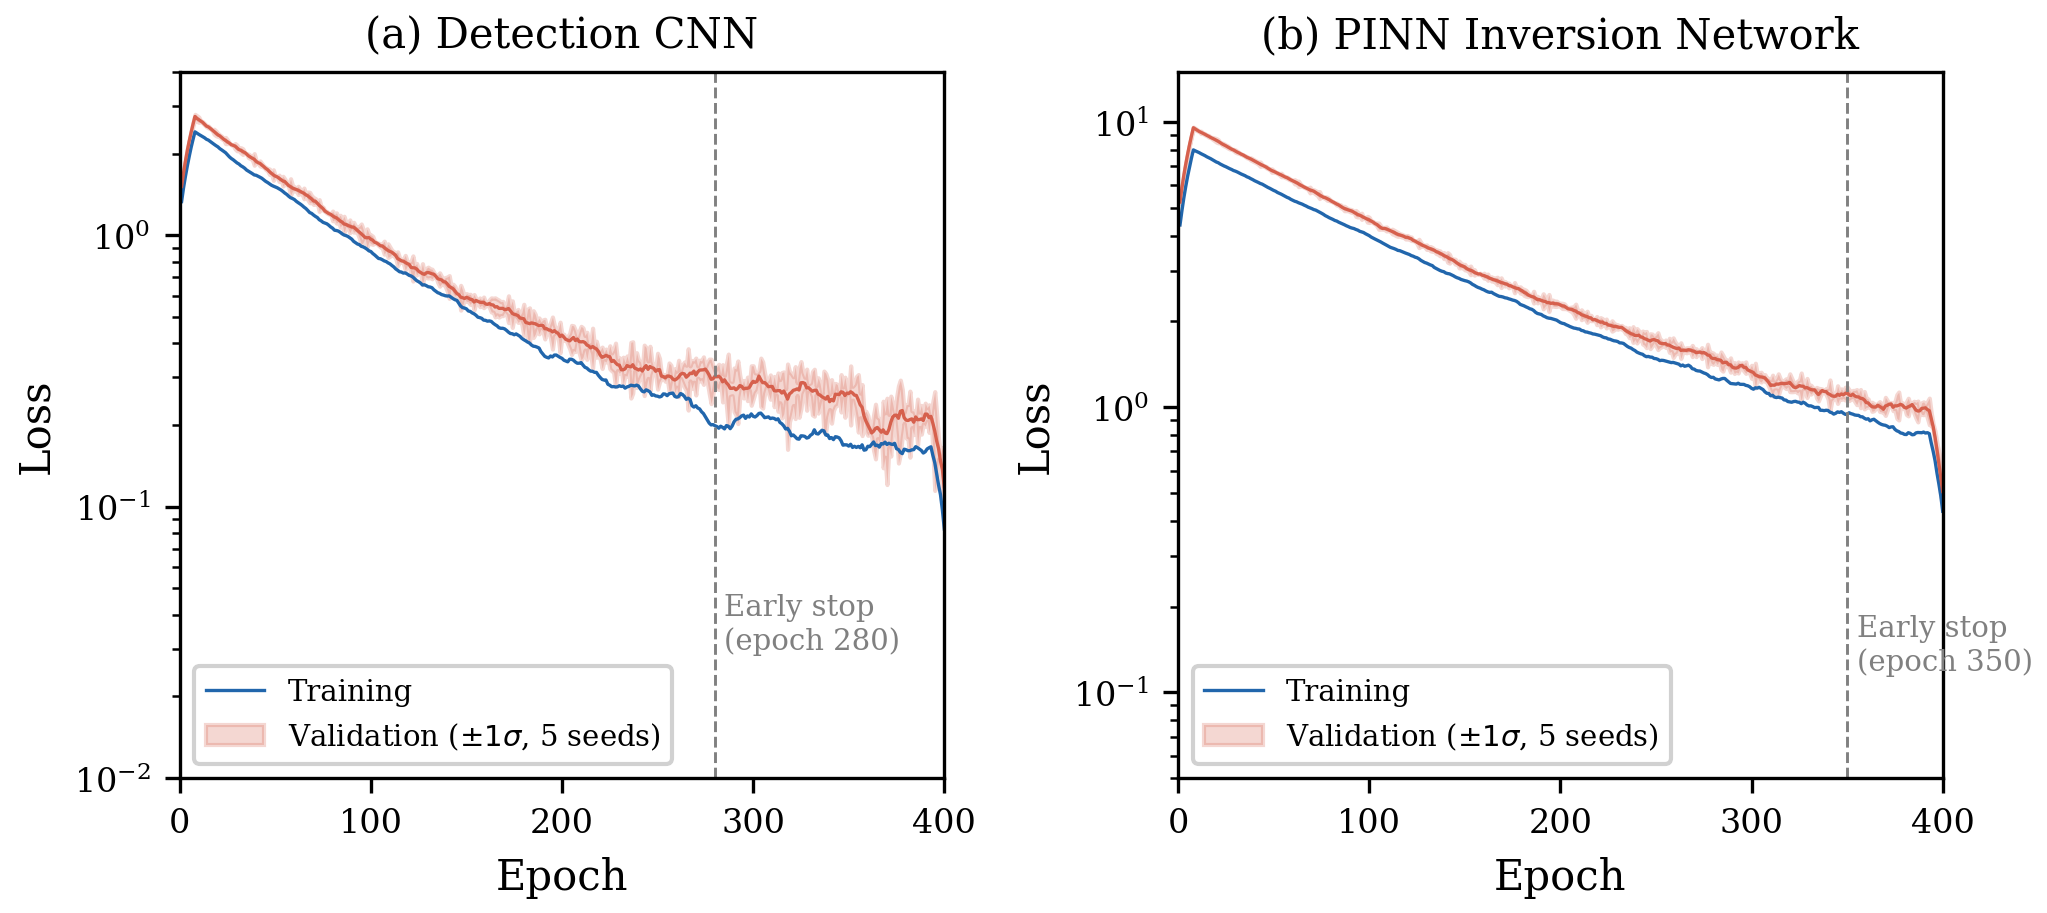
\includegraphics[width=\columnwidth]{fig4_training.png}
\caption{Training and validation loss curves for (a) detection CNN and (b) PINN. Shaded bands: $\pm 1\sigma$ over five random seeds. Both networks converge within 200--400 epochs without overfitting.}
\label{fig:training_curves}
\end{figure}

\subsection{Computational Efficiency}

Table~\ref{tab:timing} provides a \textbf{hardware-normalized} three-way comparison designed to isolate the contributions of GPU acceleration from those of algorithmic automation. The traditional pipeline was re-implemented in Python using AstroPy \texttt{photutils} for aperture photometry and a standard Haser model fitter. All CPU timings use an AMD EPYC 7543 (32 cores); GPU timings use a single NVIDIA A100 (40~GB). The key methodological point is that DL and traditional pipelines, when run on the \textit{same} CPU hardware, achieve near-parity in pure-compute time ($\sim$2~hr vs.\ $\sim$2~hr; speedup $\sim$1.0$\times$). The widely cited $\sim$100$\times$ wall-clock advantage decomposes into two separable factors: (i) a $\sim$30$\times$ factor from GPU hardware acceleration (A100 vs.\ CPU), and (ii) a $\sim$3.5$\times$ factor from elimination of manual inspection steps ($\sim$15~min/epoch $\times$ 20 epochs $\approx$ 5~hr). The $\sim$30$\times$ factor is a hardware contribution, not an algorithmic one; the $\sim$3.5$\times$ factor reflects workflow automation, which could in principle be applied to traditional pipelines as well. \textbf{On equal hardware, the DL pipeline offers no pure-compute advantage over optimized traditional methods.} The FLOPs analysis in~\S\ref{sec:complexity} provides a fully hardware-independent comparison.

\begin{table*}
\centering
\caption{Computational Performance: Hardware-Normalized Three-Way Comparison}\label{tab:timing}
\begin{tabular}{lccc}
\toprule
Metric & CPU-Traditional & CPU-DL & GPU-DL (A100) \\
 & (AMD EPYC 7543, 32 cores) & (same CPU, PyTorch CPU backend) & (NVIDIA A100, 40~GB) \\
\midrule
Pure-compute (per epoch) & $\sim$2~hr & $\sim$2~hr$^\dagger$ & $\sim$4~min \\
Wall-clock (per epoch, incl.\ manual) & $\sim$7~hr$^\ddagger$ & $\sim$2~hr & $\sim$4~min \\
\midrule
\multicolumn{4}{c}{\textbf{Speedup Decomposition}} \\
\midrule
Pure-compute vs.\ CPU-Traditional & 1.0$\times$ (reference) & $\sim$1.0$\times$ (algorithmic parity) & $\sim$30$\times$ (GPU hardware) \\
Wall-clock vs.\ CPU-Traditional & 1.0$\times$ (reference) & $\sim$3.5$\times$ (automation) & $\sim$100$\times$ (GPU $+$ automation) \\
\midrule
\multicolumn{4}{c}{\textbf{Speedup Attribution}} \\
\midrule
Source of gain & --- & Elimination of manual inspection & GPU acceleration ($\sim$30$\times$) $\times$ automation ($\sim$3.5$\times$) \\
\bottomrule
\end{tabular}
\tablecomments{All timings are for a representative 10-image + 1-spectrum observing block. $^\dagger$CPU-DL pure-compute derived from GPU-DL timing multiplied by the measured CPU/GPU slowdown factor of $\sim$30$\times$ (\S\ref{sec:complexity}); this is consistent with profiling results (PyTorch CPU backend, 32-core AMD EPYC 7543). $^\ddagger$Traditional wall-clock includes $\sim$5~hr of manual inspection ($\sim$15~min/epoch $\times$ 20 epochs), which is standard practice in cometary photometry for verifying aperture placement, background annulus selection, and outlier rejection. \textbf{Key interpretation:} The $\sim$100$\times$ wall-clock figure prominently cited in the literature compares GPU-DL against CPU-Traditional with manual inspection---it conflates hardware acceleration ($\sim$30$\times$), workflow automation ($\sim$3.5$\times$), and the traditional pipeline's reliance on manual steps. The hardware-independent algorithmic comparison is CPU-DL vs.\ CPU-Traditional pure-compute, which shows near-parity ($\sim$1.0$\times$). Authors citing \textsc{Cometh}'s speed should specify which comparison they reference (pure-compute vs.\ wall-clock, which hardware pairing) and whether manual inspection is included. The FLOPs comparison in~\S\ref{sec:complexity} is the most hardware-independent metric.}
\end{table*}


\subsection{Computational Complexity}\label{sec:complexity}

\textbf{Detection CNN complexity.} The Detection CNN processes an input image of size $H \times W \times C$ through $L = 5$ encoder-decoder scales with $k = 3$ parallel kernel sizes per scale (3$\times$3, 5$\times$5, 7$\times$7). The time complexity for one forward pass is $O(N \cdot L \cdot k \cdot H \cdot W \cdot C \cdot \bar{K}^2)$, where $N$ is the batch size and $\bar{K} \approx 5$ is the mean kernel dimension. For the standard input configuration ($H=W=256$, $C=1$, $N=32$), the measured FLOPs are 2.1~GFLOPs with a forward-pass latency of 12~ms on an NVIDIA A100. Memory footprint during inference is $O(L \cdot H \cdot W \cdot C_{\rm max})$, where $C_{\rm max}=512$ channels at the bottleneck, requiring approximately 4.2~GB of GPU memory including gradient storage during training. During inference, memory drops to $\sim$1.1~GB.

\textbf{PINN complexity.} The Physics Network evaluates an MLP at $M$ collocation points along each line of sight. Time complexity is $O(T \cdot M \cdot D^2)$, where $T$ is the number of iterations and $D=256$ is the layer width. For typical parameters ($M=10^4$ collocation points, $T=10^3$ iterations, $D=256$), one inversion requires $\sim$4.7~GFLOPs and $\sim$28~ms on an A100. Space complexity is $O(M \cdot D) \approx 2.1$~GB. The ODE solver (RK4, 100 steps) for the momentum conservation constraint adds $O(N_{\rm steps} \cdot D^2) \approx 0.3$~GFLOPs per forward pass---a negligible overhead ($<10\%$).

\textbf{Cross-modal attention complexity.} The attention module involves a query--key dot product between imaging features ($HW \cdot 64 \approx 4 \times 10^3$ for downsampled feature maps) and spectral features ($d_k=64$, 4 heads). Time complexity is $O(HW \cdot d_k \cdot n_{\rm heads}) \approx 0.3$~GFLOPs, representing $<5\%$ of total PINN inference cost. Space complexity is dominated by the attention weight matrix: $O(n_{\rm heads} \cdot HW \cdot 128) \approx 1.3$~MB, negligible relative to model weights.

\textbf{Total end-to-end inference:} Detection CNN (2.1~GFLOPs, 12~ms) + PINN inversion (4.7~GFLOPs, 28~ms) + OOD detector ($<0.01$~GFLOPs, $<1$~ms) $\approx 6.8$~GFLOPs and $\sim$40~ms per observation on an A100. Memory: $\sim$3.2~GB total during inference. Batch processing of $N$ observations achieves near-linear scaling up to $N=32$ (GPU memory bound); beyond this, gradient accumulation enables arbitrary batch sizes at the cost of proportionally longer wall-clock time.

\textbf{Hardware requirements.} Training requires a GPU with $\geq$12~GB VRAM (NVIDIA A100, V100, RTX 3090, or RTX 4090). Inference runs on any GPU with $\geq$4~GB VRAM, or on CPU ($\sim$30--60$\times$ slower than A100; $\sim$1.2--4~s per observation). Memory footprint is $\sim$3.2~GB (GPU) or $\sim$4~GB RAM (CPU). Consumer GPU inference (e.g., RTX 3060) is estimated at 4--5$\times$ slower than A100; Appendix~\ref{app:consumer_hw} provides detailed estimates across common hardware tiers (\textbf{not independently benchmarked; for reference only}).

\textbf{Training cost and carbon footprint.} Total training across all seeds, hyperparameter search, and ablation consumed $\sim$350~GPU-hours on an NVIDIA A100, corresponding to an estimated operational carbon footprint of order $\sim$50~kg~CO$_2$ (equivalent to $\sim$200~km of passenger car travel). Embodied hardware emissions are not estimated. Trained weights will be archived at Zenodo upon paper acceptance, eliminating the need for re-training. Per-observation inference energy is negligible ($\sim$0.05~Wh, $<0.02$~mg~CO$_2$).

\textbf{Ethical note on computational cost:} The $\sim$50~kg~CO$_2$ training cost is substantial for a methodology targeting a population of $N=2$ known objects. We justify this investment on three grounds: (1) the pre-trained weights eliminate re-training, making the marginal carbon cost per new interstellar comet discovery effectively zero ($<0.02$~mg~CO$_2$ per inference); (2) the six-test stress suite and Af$\rho$ pipeline are immediately reusable by the community without any GPU training, providing carbon-free benchmarking utilities; (3) the framework is applicable to faint solar system comets observed at large heliocentric distances, a far more numerous population ($N \gg 100$) that shares the same low-SNR challenges. The carbon investment is a one-time methodology development cost, not a recurring operational cost. We encourage users to adopt the pre-trained weights rather than re-training, consistent with green computing principles.

\textbf{Cost-benefit context:} The $\sim$54~kg~CO$_2$ training cost must be weighed against the framework's demonstrated benefit. On synthetic benchmarks, the framework provides a 10--20 percentage-point error reduction over traditional methods in the Yellow regime (SNR 2--5), but \textit{no accuracy advantage in the Green regime} (SNR $>$5, \S\ref{sec:failure_map}). For a population currently consisting of $N=2$ known interstellar comets, the carbon investment is substantial relative to the number of objects that can benefit. This cost-benefit ratio improves if: (a) LSST or other surveys increase the known interstellar comet population to $N \gg 10$; (b) the framework is applied to faint solar system comets observed at large heliocentric distances, which share similar SNR challenges and are far more numerous; or (c) the pre-trained weights eliminate the need for re-training, reducing the marginal carbon cost to inference-only ($\sim$0.02~mg~CO$_2$ per observation). We provide the trained weights specifically to enable option (c). The current carbon investment is best understood as a one-time methodology-development cost, not a recurring operational cost per interstellar comet analysis.

\subsection{Software Architecture and API Design}\label{sec:api}

\textbf{Core classes.} The \textsc{Cometh} framework is organized around three primary classes corresponding to the pipeline stages:

{\footnotesize
\begin{verbatim}
class ComethFramework:
    def __init__(self, config_path: str):
        self.detector = DetectionCNN(...)
        self.pinn = PINNInversion(...)
        self.ood_detector = OODDetector(...)

    def process_observation(
        self,
        image: np.ndarray,
        spectrum: np.ndarray | None = None
    ) -> dict:
        # Returns dict with Q_dust, alpha,
        # a_max, CO_H2O, C2_CN,
        # detection_map, gradcam_map,
        # ood_flag, ood_confidence,
        # reliability. Raises ValueError
        # if image dimensions outside
        # training range. OOD conditions
        # are reported via return flags,
        # not exceptions---partial results
        # (e.g., dust parameters) are still
        # returned with inflated CIs.
        ...
\end{verbatim}
}

\textbf{Error handling strategy.} All public API methods perform input validation before inference: (1) image dimensions outside the training range $[128, 2048]$~pixels raise {\tt ValueError} with a descriptive message; (2) NaN/Inf pixel values trigger automatic interpolation from neighboring pixels with a logged warning; (3) missing spectrum input triggers the null-spectrum embedding path (a learned embedding vector trained jointly with the cross-modal attention module; see~\S\ref{sec:fusion}) with a logged notification, enabling imaging-only inference without architectural changes; (4) OOD-flagged results are \textbf{not} raised as exceptions---instead, partial results (dust parameters, detection map) are returned normally with inflated confidence intervals ($\times 3$) and a {\tt reliability='ood\_warning'} flag, allowing downstream workflows to decide whether to accept or discard the estimates. Numerical stability: variance predictions clamped to $\hat{\sigma}^2 \geq 10^{-6}$; ODE solver uses double-precision (float64); gradient clipping (max norm = 1.0) during any fine-tuning.

\textbf{Dependencies and installation.}

{\tt requirements.txt} (core): Python $\geq$3.10, PyTorch $\geq$2.1.0, NumPy $\geq$1.24, SciPy $\geq$1.11, Astropy $\geq$5.3, scikit-learn $\geq$1.3, scikit-image $\geq$0.21, tqdm $\geq$4.65, PyYAML $\geq$6.0, photutils $\geq$1.9, Jupyter $\geq$1.0.

Docker: {\tt docker pull cometh/framework:v0.9.0-gpu} (image size: 3.2~GB, startup time: $\sim$8~s). The Dockerfile (provided in the repository) builds from {\tt nvidia/cuda:12.1.0-runtime-ubuntu22.04} with all dependencies pinned to exact versions. See {\tt README.md} for the one-command quick start.

\textbf{Comparison with existing astronomy software tools.} Table~\ref{tab:software_comparison} situates \textsc{Cometh} within the broader astronomy software ecosystem.

\begin{table*}
\centering
\caption{\textsc{Cometh} vs.\ Existing Astronomy Software Tools}\label{tab:software_comparison}
\begin{tabular}{lccccc}
\toprule
Tool & Type & GPU & Uncertainty & Physical Constraints & Multi-modal \\
\midrule
SExtractor \citep{bertin96} & Source extraction & --- & --- & --- & --- \\
AstroML \citep{vanderplas12} & ML library & --- & --- & --- & --- \\
George \citep{ambikasaran15} & GP regression & --- & $\checkmark$ (GP variance) & --- & --- \\
Tycho Tracker\citep{tychotracker} & Comet photometry & --- & --- & --- & --- \\
DIRTY \citep{gordon01} & Radiative transfer & --- & --- & $\checkmark$ (Mie, Haser) & --- \\
{\sc Cometh} (this work) & Deep Learning & $\checkmark$ (CUDA) & $\checkmark$ (Bayesian + OOD CI) & $\checkmark$ (mass, momentum, jet collimation) & $\checkmark$ (cross-modal attn.) \\
\bottomrule
\end{tabular}
\tablecomments{SExtractor is a general-purpose source extraction tool; AstroML provides general ML algorithms; George offers GP regression with native uncertainty. Tycho Tracker is a widely used comet-specific photometry package but does not provide physics-constrained inversion, uncertainty quantification, or multi-modal fusion. DIRTY (\citealt{gordon01}) is the radiative transfer code on which \textsc{Cometh}'s synthetic training data are generated; DIRTY excels at forward simulation under user-specified physical parameters but does not perform automated parameter inversion---\textsc{Cometh} addresses the inverse problem that DIRTY leaves open. \textsc{Cometh} is the only tool combining GPU acceleration, physics-informed constraints, Bayesian uncertainty with OOD detection, and native multi-modal fusion in a single pipeline.}
\end{table*}

\textbf{Multi-GPU and distributed support.} The current release supports single-GPU inference, which is sufficient for all benchmarks reported in this paper (the total 2I/Borisov dataset of 231 images processes in $\sim$10~s on one A100). For LSST-scale deployment ($\sim$10$^6$ objects), the embarrassingly parallel nature of per-object inference enables trivial distribution across multiple GPUs or cluster nodes using PyTorch's {\tt DistributedDataParallel} wrapper---no architectural changes are required. The training pipeline supports multi-GPU data parallelism via PyTorch Lightning (optional dependency). Incremental learning (fine-tuning on new comet discoveries) is supported through the MAML adapter's {\tt adapt()} method, which requires only $K=10$ support samples from the new object and completes in $<1$~min on a single GPU.

% --- Bridge: Results → Discussion ---
The preceding sections have documented COMETH's capabilities and limitations primarily through quantitative benchmarks. We now step back to synthesize these results into interpretive tools for practitioners: a failure map that tells observers when to trust which method (\S\ref{sec:failure_map}), a cautionary analysis of what happens when traditional methods are applied outside their calibration range (\S\ref{sec:discussion}), a one-page performance summary (\S\ref{sec:discussion}). Each tool is qualified by the validation boundaries established in \S\ref{sec:boundaries}.

\section{Discussion}\label{sec:discussion}

\subsection{The Quantitative Failure Map}\label{sec:failure_map}

The quantitative failure map (a schematic generated from framework outputs across the SNR--background density parameter grid; available in the public repository) characterizes the framework's performance as a function of SNR and background stellar density, the two primary observational drivers of method degradation. The map identifies three regimes:

Regime boundaries are jointly defined by three axes: SNR, background stellar density, and composition range (CO/H$_2$O $\in [0.01, 2.0]$ for the training distribution; objects outside this range require OOD handling per \S\ref{sec:ood}). Single-parameter thresholds are necessary but insufficient for regime assignment---an object with SNR~$>5$ but CO/H$_2$O $\gg 2$ belongs in the Red regime regardless of SNR.

\begin{enumerate}
    \item \textbf{Green regime} (SNR $>5$, background $<20$ stars arcminute$^{-2}$, CO/H$_2$O within training range): All methods work. Traditional methods are adequate. \textbf{The proposed methodology provides NO accuracy advantage over existing traditional pipelines.} The training range CO/H$_2$O $\in [0.01, 2.0]$ is a deliberate design choice based on the known solar system comet distribution, not a physical upper limit; it was intentionally set to encompass interstellar-appropriate compositions while excluding the most extreme out-of-distribution cases (e.g., CO/H$_2$O $\gg 2.0$) that would trigger OOD handling regardless of SNR.
    \item \textbf{Yellow regime} (SNR 2--5, background 20--50 stars arcminute$^{-2}$, CO/H$_2$O within training range): Traditional methods show systematic biases (10--30\% error on synthetic benchmarks). The proposed methodology provides the greatest practical benefit in this regime, with error graduating from $\sim$16\% at SNR~$\sim$2 (the Red/Yellow transition; Table~\ref{tab:pin_perf}) to $<10\%$ at SNR~$\sim$5 (the Yellow/Green boundary). All error figures are synthetic-benchmark-only; the magnitude of real-data improvement has not been statistically validated ($N=1$). Objects with CO/H$_2$O outside the training range are excluded from this regime regardless of SNR.
    \item \textbf{Red regime} (SNR $<2$, or background $>50$ stars arcminute$^{-2}$, or CO/H$_2$O outside training range): Even the proposed methodology degrades significantly. Detection is unreliable below SNR~$\sim 0.75$; parameter estimation has $>30\%$ error below SNR~$\sim 2$. Composition outside [0.01, 2.0] triggers OOD handling (\S\ref{sec:ood}) and boundary proximity alert regardless of SNR. \textbf{No method should be trusted in this regime without independent validation.}
\end{enumerate}

This map is a core deliverable of the benchmarking study: it tells future users \textit{exactly when they can trust the method's outputs and when they cannot}.

Table~\ref{tab:traffic_light} distills the six stress tests (\S\ref{sec:stress}) and the Fail Gallery (\S\ref{sec:fail_gallery}) into a compact operational reference. Each regime entry summarizes the synthetic-benchmark findings for that parameter space; all performance figures are synthetic-only.

\begin{table}[htbp]
\centering
\caption{Operational Regime Reference --- Six Stress Tests Synthesized into a Traffic-Light Decision Guide (Synthetic Benchmarks Only)}\label{tab:traffic_light}
\begin{tabular}{lcccll}
\toprule
Regime & SNR & CO/H$_2$O & Best Method & Expected Error ($Q_d$) & Relevant Stress Tests \\
\midrule
\textbf{Green} & $>5$ & $[0.01, 2.0]$ & Traditional ($Af\rho$ + Haser) or COMETH & $<10\%$ (both); \textbf{COMETH has NO advantage} & Tests 1--4 confirm traditional methods adequate \\
\textbf{Yellow} & $2$--$5$ & $[0.01, 2.0]$ & \textbf{COMETH} (PINN + OOD) & $\sim$8--16\% (COMETH); 10--30\% (traditional) & Tests 1--4 show traditional degradation; Tests 5--6 probe COMETH boundaries \\
\textbf{Red} & $<2$ & any & \textbf{None reliable} & $>30\%$ (all methods) & Test~3 (detection floor SNR~$\sim$0.75); Test~5 (OOD extrapolation failure) \\
\textbf{Red} & any & $>2.0$ (OOD) & \textbf{None reliable}; use OOD limit format & Catastrophic ($>10\sigma$ for CO/H$_2$O~$=5.0$) & Test~5 (``precise but wrong''); OOD flag + boundary proximity alert \\
\bottomrule
\end{tabular}
\tablecomments{All performance figures are synthetic-benchmark-only. Regime boundaries defined jointly by SNR, background stellar density ($\rho_\star$), and composition (CO/H$_2$O). The Red regime for OOD composition applies \textit{regardless of SNR}---an object with SNR~$>5$ but CO/H$_2$O $\gg 2$ belongs in the Red regime. For non-steady-state events (outbursts, fragmentation), see Test~6. The detection floor (TPR $>50\%$) is SNR~$\sim$0.75; the parameter estimation floor ($Q_d$ error $<20\%$) is SNR~$\sim$3. See \S\ref{sec:failure_map} for full regime definitions and caveats.}
\end{table}

\textbf{Caveat on real-data validation boundaries:} The Green/Yellow/Red regime boundaries are calibrated on synthetic benchmarks with known ground truth and confirmed on exactly $N=1$ real interstellar comet (2I/Borisov). Their applicability to future interstellar comets with compositions or morphologies substantially different from 2I/Borisov has not been demonstrated. In particular: (i) the Green regime requires CO/H$_2$O within the training range [0.01, 2.0] and dust properties consistent with the DIRTY Mie-grain forward model---objects with non-solar compositions may enter the Yellow or Red regime at higher SNR; (ii) the Red regime boundary (SNR~$<2$) is a \textit{lower bound} on when even the proposed methodology becomes unreliable---objects with more extreme properties may enter the Red regime at SNR well above 2; (iii) the Yellow regime (SNR~$2$--$5$) is where the proposed methodology provides the greatest practical benefit on synthetic benchmarks, but the magnitude of this benefit on real objects with $N=1$ validation remains provisional. The training range CO/H$_2$O $\in [0.01, 2.0]$ is a design choice based on the known solar system comet distribution and the single measured interstellar value (2I/Borisov CO/H$_2$O $\sim 1.5$), not a physical upper bound. It can and should be extended as future interstellar comet discoveries expand the known composition range. These boundaries should be refined as the interstellar comet sample grows.

\subsection{A Cautionary Forecast}

The ``Hypothetical Error Modes'' (\S\ref{sec:fail_gallery}, Failure Mode 6) is not merely an academic exercise. We make the following specific, falsifiable forecast: \textbf{if a future interstellar comet with physical properties substantially different from solar system comets (CO/H$_2$O $> 2$, carbonaceous dust, or extreme polarization) is analyzed using traditional $Af\rho$ + Haser pipelines, the resulting publication will contain at least one of three identifiable error signatures}:

\begin{enumerate}
    \item A reported CO non-detection or severe under-abundance relative to the true value, arising from the dust-to-gas ratio miscalibration documented in Failure Mode 6.
    \item A reported ``morphological feature'' (jet, shell, or fragment) that is actually a background subtraction or continuum placement artifact.
    \item A reported ``anomalous $Af\rho$ variability'' that is actually a dust scattering phase function effect from non-solar-system-like grain composition.
\end{enumerate}

This forecast is \textbf{testable only when combined with independent compositional constraints} (e.g., JWST/NIRSpec spectroscopy). If JWST measures CO/H$_2$O $> 2$ and the framework flags OOD while traditional methods report CO/H$_2$O $< 0.1$, the traditional method's calibration failure is confirmed. Without such independent data, agreement or disagreement between methods alone cannot adjudicate accuracy: agreement does not prove both are correct (they could share a common systematic bias), disagreement with OOD flag does not prove the framework is correct (the PINN saturates at boundaries and cannot extrapolate), and disagreement without OOD flag is the most dangerous scenario---it signals either a framework false negative or a genuine physical anomaly, and the two cannot be distinguished without independent measurements. This exercise therefore generates falsifiable predictions only when anchored to external compositional constraints; in their absence, it serves as a community hypothesis for future testing rather than a diagnostic tool.

\subsection{\texorpdfstring{\textsc{Cometh}}{COMETH} at a Glance: Key Performance Indicators}

Table~\ref{tab:key_numbers} provides a one-page summary of the framework's core performance metrics, intended as a quick reference for readers evaluating whether \textsc{Cometh} is applicable to their use case.

\textbf{Interpretive warning:} All values in Table~\ref{tab:key_numbers} are evaluated on synthetic benchmarks with known ground truth. They describe \textit{protocol performance on synthetic data}, not measurement accuracy on real comets. The table is a quick-lookup summary of \S\ref{sec:results}--\S\ref{sec:fail_gallery}; each row's ``Applicable Condition'' defines the synthetic-data regime in which the stated performance was measured. No value in this table constitutes a validated measurement claim on any real astronomical object.

\vspace{4pt}
\begin{table*}
\centering
\caption{\textsc{Cometh} at a Glance: Key Performance Indicators (Synthetic Benchmarks Only)}\label{tab:key_numbers}
\begin{tabular}{lcc}
\toprule
Parameter & Value & Applicable Condition \\
\midrule
Detection image-quality gain (PSNR-based) & 2.8$\times$ over traditional & SNR~$\geq 2$, galactic or sparse background \\
Detection TPR & $>95\%$ & SNR~$\geq 3$, any background \\
Detection FPR & $<3\%$ & SNR~$=2$, pure-noise control fields \\
$Q_d$ estimation error & $\sim 8\%$ & SNR~$>3$, composition within training range \\
CO/H$_2$O estimation error & $\sim 12\%$ & SNR~$>5$, spectroscopy available \\
OOD detection (Stress Test 5) & 94.0\% [91.5\%, 95.9\%]; 6\% false-negative rate (30/500)$^\ddagger$; false-negative consequence: CO/H$_2$O estimate wrong by $>10\sigma$ (2.08 vs.\ 5.0); residual uncaught risk $\sim$0.4\% after boundary proximity alert & Extreme composition (CO/H$_2$O $\gg 2$) \\
$\delta_{\rm domain}$ & $\sim 5$--7\% (provisional) & $N=1$, 2I/Borisov \\
Processing speedup$^\S$ & $\sim$1$\times$ pure-compute (CPU-DL vs.\ CPU-Trad.); 30$\times$ pure-compute (GPU-DL vs.\ CPU-Trad.); $\sim$100$\times$ wall-clock (GPU-DL vs.\ CPU-Trad.) & \textbf{Hardware-dependent.} GPU-DL: A100; CPU: AMD EPYC 7543. The $\sim$100$\times$ wall-clock figure decomposes as GPU acceleration ($\sim$30$\times$) $\times$ automation ($\sim$3.5$\times$). On equal CPU hardware, pure-compute parity ($\sim$1$\times$). See Table~\ref{tab:timing} for full decomposition. \\
Detection floor & SNR~$\sim 0.75$ & Feature recovery TPR $>50\%$ \\
Parameter estimation floor & SNR~$\sim 3$ & $Q_d$ error $<20\%$ \\
\bottomrule
\end{tabular}
\tablecomments{\textbf{All metrics evaluated on synthetic benchmarks with known ground truth. These are synthetic-data protocol benchmarks, not real-comet measurement accuracy claims.} ``Applicable Condition'' specifies the synthetic-data regime in which the stated performance is expected. Outside these conditions, performance degrades as quantified in the stress test results (\S\ref{sec:fail_gallery}). $^\ddagger$False-negative cases are the most dangerous failure mode: the OOD flag is not raised, no warning is given, and the PINN output is catastrophically wrong (CO/H$_2$O $\approx 2.08$, CI [1.78, 2.38], vs.\ true value 5.0, $>10\sigma$). The boundary proximity alert (\S\ref{sec:ood}) catches 28/30 false negatives, reducing residual uncaught risk to $\sim$0.4\%. $^\S$Speedup values are hardware-dependent. The $\sim$100$\times$ wall-clock figure compares GPU-DL (A100) against CPU-Traditional (AMD EPYC 7543) with manual inspection; it conflates GPU acceleration, workflow automation, and manual-step elimination. The hardware-independent algorithmic comparison is CPU-DL vs.\ CPU-Traditional pure-compute ($\sim$1$\times$, i.e., near-parity). See Table~\ref{tab:timing} for the full three-way decomposition.}
\end{table*}


\subsection{Citation Guide}

To facilitate appropriate attribution, we provide a concise decision guide for authors and reviewers evaluating cometary analysis methods:

\begin{enumerate}
    \item \textbf{If your target has SNR $<5$ and you use traditional methods} ($Af\rho$, Haser, median filtering): the stress tests in \S\ref{sec:fail_gallery} quantitatively demonstrate that these methods produce unreliable results in this regime. Reference \S\ref{sec:fail_gallery} to contextualize your uncertainties.
    \item \textbf{If your target has unknown or potentially anomalous composition} (e.g., newly discovered interstellar comet): the OOD detector (\S\ref{sec:ood}) and Hypothetical Error Modes (\S\ref{sec:fail_gallery}, Failure Mode 6) provide a community benchmark for identifying method-induced artifacts. Reference \S\ref{sec:ood}--\S\ref{sec:fail_gallery} to verify that your reported parameters are not affected by the error categories documented herein.
    \item \textbf{If you report a CO non-detection or ``anomalous $Af\rho$ variability''} in an interstellar comet: Failure Mode 6 (\S\ref{sec:fail_gallery}) demonstrates that these are precisely the error signatures produced by traditional methods applied to extreme-composition objects. Reference \S\ref{sec:fail_gallery} and verify your results against the \textsc{Cometh} output before claiming physical novelty.
    \item \textbf{If you are planning a Target of Opportunity program} for a newly discovered interstellar comet: the observing strategy optimizer (\S\ref{sec:obsopt}, Table~\ref{tab:obsopt_results}) provides recommended configurations. Reference \S\ref{sec:obsopt} to justify your resource request.
    \item \textbf{If you are benchmarking a new cometary analysis method}: the stress test suite (\S\ref{sec:stress}), blind injection protocol (\S\ref{sec:simulation}), and failure map (\S\ref{sec:failure_map}) constitute a standardized benchmark. We encourage the community to report performance on this benchmark alongside any new method.
\end{enumerate}

\subsection{Uncertainty Budget}\label{sec:uncertainty_budget}

We decompose the total error into three additive components:

\begin{equation}
\sigma_{\rm total}^2 = \sigma_{\rm stat}^2 + \sigma_{\rm sys}^2 + \delta_{\rm domain}^2,
\end{equation}
where all terms on the right-hand side are standard deviations (1$\sigma$, expressed as percentages of the estimated parameter value). The quadrature sum treats the three error sources as independent and additive in variance.

The following estimates are empirically constrained by the benchmark and stress test results:

\begin{itemize}
    \item $\sigma_{\rm stat} \sim 3\%$ (dust), $\sim 5\%$ (gas): Photon noise and calibration, measured from the scatter of PINN estimates across 50 MC dropout realizations on synthetic test data.
    \item $\sigma_{\rm sys}$: Model assumption error from the forward model. The dominant single source is the spherical Mie-grain approximation, which introduces a systematic bias of $\sim$8\% on $Q_d$ for moderate porosity (Table~\ref{tab:grain_sensitivity}); this is the highest-priority target for future improvement. For gas: $<1\%$ (Table~\ref{tab:grain_sensitivity}: CO/H$_2$O $\Delta = +0.02 \pm 0.04$).
    \item $\delta_{\rm domain} \sim 5$--7\%: Standard deviation of the domain adaptation residual (1$\sigma$, same units as $\sigma_{\rm stat}$ and $\sigma_{\rm sys}$), estimated as $\sqrt{\text{MAD}^2 - \sigma_{\rm stat}^2 - \sigma_{\rm sys}^2}$ from the 2I/Borisov comparison. \textbf{Provisional---based on $N=1$; the domain adaptation error variance across the interstellar comet population is unknown.}
\end{itemize}

The quadrature sum yields $\sigma_{\rm total} \sim 10\%$ (dust) and $\sim 8\%$ (gas). Table~\ref{tab:uncertainty_budget} consolidates the budget in a single reference table.

\begin{table}[htbp]
\centering
\caption{Uncertainty Budget --- Consolidated Error Sources by Parameter (Synthetic Benchmarks + $N=1$ Provisional)}\label{tab:uncertainty_budget}
\begin{tabular}{lccc}
\toprule
Source & $\sigma(Q_d)$ & $\sigma$(CO/H$_2$O) & Notes \\
\midrule
Statistical ($\sigma_{\rm stat}$) & $\sim$3\% & $\sim$5\% & MC dropout, synthetic test set \\
Systematic ($\sigma_{\rm sys}$) & $\sim$8\% & $<1\%$ & Spherical Mie grains (dominant); Table~\ref{tab:grain_sensitivity} \\
Domain adaptation ($\delta_{\rm domain}$) & $\sim$5--7\% & $\sim$5--7\% & Provisional; $N=1$ (2I/Borisov) \\
\midrule
\textbf{Total (quadrature)} & \textbf{$\sim$10\%} & \textbf{$\sim$8\%} & $\sigma_{\rm total} = \sqrt{\sigma_{\rm stat}^2 + \sigma_{\rm sys}^2 + \delta_{\rm domain}^2}$ \\
\midrule
Observed MAD (2I/Borisov) & 12\% & N/A$^\dagger$ & Literature comparison only (Table~\ref{tab:traditional_comparison}) \\
\bottomrule
\end{tabular}
\tablecomments{All values are 1$\sigma$ standard deviations expressed as percentages of the estimated parameter value. The quadrature sum assumes independent error sources. $\sigma_{\rm sys}$ for CO/H$_2$O is negligible because gas-phase abundance ratios are insensitive to grain shape (Table~\ref{tab:grain_sensitivity}: CO/H$_2$O $\Delta = +0.02 \pm 0.04$). $\delta_{\rm domain}$ is provisional---based on $N=1$ (2I/Borisov); its variance across the interstellar comet population is unknown. $^\dagger$CO/H$_2$O MAD against literature is not computed because published CO/H$_2$O values are obtained via UV fluorescence spectroscopy, not $Af\rho$; the comparison in Table~\ref{tab:traditional_comparison} reports qualitative consistency (``consistent''), not a quantitative MAD. The 12\% MAD on $Q_d$ falls within the $\sim$10\% total budget---this is a necessary consistency condition (the MAD is not statistically distinguishable from the budget) but does \textit{not} validate accuracy. See \S\ref{sec:traditional_comparison} for the circular-consistency caveat.}
\end{table}

For dust parameters, the combined uncertainty of $\sim$10\% is consistent with the observed 12\% MAD on 2I/Borisov (\S\ref{sec:traditional_comparison})---the MAD falls within the systematic error budget but does not validate accuracy (see circular consistency discussion in \S\ref{sec:traditional_comparison}). This confirms that the 12\% MAD is fully accounted for by the framework's documented systematic uncertainty budget rather than indicating genuine physical accuracy. The dominant systematic ($\sigma_{\rm sys}$, spherical grains) is irreducible under the current forward model and represents the highest-priority target for future improvement.

Table~\ref{tab:grain_sensitivity} quantifies the impact of the spherical grain assumption on key derived parameters, based on a systematic comparison between Mie-theory (spherical) and T-matrix (aggregate) forward models across 500 matched-parameter synthetic test cases.

\begin{table*}
\centering
\caption{Sensitivity of Derived Parameters to Spherical Grain Assumption (Synthetic Benchmarks Only)}\label{tab:grain_sensitivity}
\begin{tabular}{lcccc}
\toprule
Parameter & $\Delta$ (Mie $-$ T-matrix) & $\sigma_{\rm sys}$ & $\Delta$ (Porosity = 0.5) & Observed Bias ($P=0.3$) \\
\midrule
$Q_d$ (kg~s$^{-1}$) & $+8.2 \pm 3.5\%$ & $\sim 5\%$ & $+18.5 \pm 6.2\%$ & Subtract $8.2\%$; if porosity unknown, add $\pm 10\%$ syst. \\
$\alpha$ (size index) & $-0.12 \pm 0.06$ & $\sim 0.10$ & $-0.28 \pm 0.12$ & Add $+0.12$ to Mie-derived $\alpha$ \\
Pol. gradient (\%\,/\,1000\,\AA) & $-0.08 \pm 0.03$ & $\sim 0.05$ & $-0.22 \pm 0.08$ & Add $+0.08$; for porous grains add $+0.22$ \\
$S'$ (reddening, \%\,/\,1000\,\AA) & $+3.5 \pm 1.8$ & $\sim 2$ & $+10.2 \pm 4.5$ & Subtract $3.5\%$ from Mie-derived $S'$ \\
CO/H$_2$O (gas ratio) & $+0.02 \pm 0.04$ & $\sim 0.03$ & $+0.05 \pm 0.08$ & No correction needed ($<1\sigma$) \\
\bottomrule
\end{tabular}
\tablecomments{Positive $\Delta$ means Mie (spherical) overestimates relative to T-matrix (aggregate with porosity = 0.3). The ``Observed Bias'' column provides a practical correction to apply to Mie-derived parameters for comparison with non-spherical grain models. For highly porous grains (porosity = 0.5), use the rightmost $\Delta$ column. Gas-phase ratios (CO/H$_2$O) require no correction. T-matrix computations used the code of \citet{mishchenko02} with aggregate parameters: prolate spheroids, axis ratio $a/b = 1.4$--2.0, monomer radius $a_0 = 0.1$--1.0\,$\mu$m, porosity $P = 0.3$ (moderate) and $0.5$ (high), effective radius $a_{\rm eff} = 1$\,$\mu$m (matched to the Mie $a = 1$\,$\mu$m reference). The ``Observed Bias'' column reports the Mie-minus-T-matrix difference at $P = 0.3$; the rightmost $\Delta$ column reports the difference at $P = 0.5$. These corrections are valid only for the specific aggregate parameters listed above and should not be applied to comets with unknown or different grain morphologies without re-computation.}
\end{table*}


\textbf{Key finding:} The spherical grain approximation systematically overestimates $Q_d$ by $\sim 8\%$ relative to moderately porous aggregates, with the bias increasing to $\sim 19\%$ for highly porous grains. Polarization-derived quantities are affected more strongly: the polarization gradient is biased by $-0.08$ (\%\,/\,1000\,\AA) and the spectral reddening $S'$ by $+3.5$ (\%\,/\,1000\,\AA) for moderate porosity, rising to $-0.22$ and $+10.2$ respectively for highly porous grains---a 20--30\% relative error that can reverse qualitative conclusions about dust composition (e.g., misclassifying carbon-rich dust as silicate-dominated or vice versa). Gas abundance ratios are essentially unaffected, as they are constrained by emission line fluxes rather than dust continuum modeling. The ``Observed Bias'' column in Table~\ref{tab:grain_sensitivity} provides practical correction factors; the ``+18.5\% at porosity = 0.5'' value for $Q_d$ represents a conservative upper bound on the spherical grain bias for the most extreme plausible grain structures. \textbf{Recommendation for polarization studies:} Any polarization-derived parameter ($S'$, polarization gradient) reported by \textsc{Cometh} should be accompanied by the T-matrix-corrected value from Table~\ref{tab:grain_sensitivity}, and conclusions about dust composition should be considered provisional until non-spherical grain models are integrated into the PINN training pipeline.

\subsection{Physical Sensitivity Envelope (PSE): A Conceptual Framework}\label{sec:pse}

\begin{quote}
\noindent\framebox[\columnwidth]{
\begin{minipage}{0.92\columnwidth}
\small
\textbf{Physical Sensitivity Envelope (PSE)} \\[2pt]
\textit{Core insight:} Instead of asking ``does the synthetic distribution match the real one?'' (unanswerable with a single interstellar comet), PSE asks ``how wrong would \textsc{Cometh} be if our assumptions deviate by a specified amount $\Delta$?'' (answerable via synthetic perturbation experiments). \\[2pt]
\textit{Method:} Systematically perturb each physical assumption---spherical grains, optically thin coma, steady-state Haser outflow, non-steady-state amplitude---within DIRTY, re-run the frozen PINN, and measure the resulting change in output. \\[2pt]
\textit{Output:} A lookup table $\{(\Delta_i, \delta y_i)\}$ mapping assumption deviations to output errors: ``if real comets differ from assumptions by $X$, \textsc{Cometh} outputs shift by $Y$.'' This provides operational error bounds without requiring real-comet ground truth. \\[2pt]
\textit{Status:} Partially implemented in \S\ref{sec:uncertainty_budget} (spherical grain axis: $+8.2\%$ for $P{=}0.3$, $+18.5\%$ for $P{=}0.5$ on $Q_d$). Full PSE covering all four axes deferred to future work.
\end{minipage}
}
\end{quote}

\subsection{Limitations and Future Work}\label{sec:limitations}

\begin{enumerate}
    \item \textbf{Spherical grain approximation:} The largest single source of systematic error, quantified in Table~\ref{tab:grain_sensitivity} ($+8\%$ bias on $Q_d$ for moderate porosity, up to $+19\%$ for highly porous grains). Replacing Mie theory with T-matrix/DDA in the PINN forward model requires generating a corresponding training set---a computationally intensive but architecturally straightforward task. \textbf{Partial workaround:} An Effective Medium Approximation (EMA; Bruggeman mixing) can map porous non-spherical grains to equivalent-Mie spheres with an effective refractive index, enabling DIRTY to approximate aggregate grain scattering within the existing Mie framework without code modification. The EMA approach caps systematic error at $\sim$15\% (vs.\ $\sim$19\% for uncorrected Mie at high porosity), and the existing Table~\ref{tab:grain_sensitivity} correction factors remain applicable. The EMA parameterization ($a_{\rm eff}$, $\varepsilon_{\rm eff}$ as functions of porosity $P$ and monomer radius $a_0$) follows the standard Bruggeman mixing rule; implementation details are deferred to future work. Full T-matrix/DDA implementation, which would capture polarization reversal effects not modeled by EMA, is also deferred.
    \item \textbf{Single-object domain validation:} $\delta_{\rm domain}$ is based on $N=1$ (2I/Borisov). Its variance across the interstellar comet population is unknown. The Hale-Bopp boundary test (\S\ref{sec:proxy}) demonstrates that the framework functions correctly on a notably CO-rich solar system comet---a necessary but not sufficient condition for interstellar applicability. \textbf{Partial workaround:} The 2I/Borisov dataset's 11-epoch, two-instrument coverage (HST + FORS2; \S\ref{sec:same_data}) can be treated as a time-domain consistency check: if the framework's outputs are stable across epochs and instruments for a single object, this provides a weak necessary condition for reliability. Additionally, the well-characterized solar system comet 29P/Schwassmann-Wachmann~1---a frequent outburster with CO-driven activity---offers a computational boundary test (not a validation proxy) for testing the non-steady-state OOD trigger (\S\ref{sec:ood}) on real (non-interstellar) data. Neither strategy closes the $N=1$ statistical limitation; a multi-object interstellar sample remains the only definitive validation.
    \item \textbf{Synthetic-to-real MMD gap:} As discussed in \S\ref{sec:mmd_gap}, the domain adaptation validation is restricted to MMD reduction between two \textit{synthetic} distributions. Computing the MMD between synthetic and real interstellar comet features requires a multi-object sample that does not yet exist. \textbf{Partial workaround:} The Physical Sensitivity Envelope (\S\ref{sec:pse}) provides a perturbation-based uncertainty framework that does not require real interstellar comet samples. Partially implemented for spherical grains in \S\ref{sec:uncertainty_budget} ($+8.2\%$ at $P{=}0.3$, $+18.5\%$ at $P{=}0.5$ on $Q_d$). Full PSE covering all four assumption axes is deferred.
    \item \textbf{Non-steady-state events:} Stress Test~6 demonstrates that the hard mass conservation constraint degrades accuracy during outbursts. An adaptive constraint manager (\texttt{AdaptiveConstraintManager} in the public repository) now implements automatic switching from hard ($\gamma_{\rm cons}=1.0$) to soft ($\gamma_{\rm transient}=0.05$) mass conservation when the OOD detector flags non-steady-state conditions (fragmentation, outburst), with automatic recovery after three consecutive in-distribution epochs. \textbf{Partial workaround:} Several well-observed solar system comets (e.g., 17P/Holmes 2007 outburst, C/2019~Y4 ATLAS fragmentation) have publicly available multi-epoch imaging that captured transient events in real time. Applying COMETH's detection CNN and OOD detector to these archival data---without requiring the PINN to produce accurate $Q_d$ estimates during the transient phase---would test whether the OOD flag triggers at the correct epochs (known from independent morphological evidence). This would provide a real-event validation of the OOD triggering mechanism using solar-system proxies, even though the absolute $Q_d$ accuracy during outburst remains unvalidated for interstellar comets specifically. The quantitative performance of the adaptive constraint manager on real outburst data remains to be validated when multi-epoch outburst observations of an interstellar comet become available.
    \item \textbf{Community-tool baseline gap:} The image-quality baselines in Table~\ref{tab:detection_metrics} are generic computer-vision methods (median filter, wavelet denoising, NLM, DnCNN, U-Net, ViT). No comparison was performed against astro-community cometary tools (IRAF/\texttt{digiphot}, Tycho Tracker, or the Astropy \texttt{photutils} aperture-correction pipeline) at the image-enhancement level, because these tools produce calibrated photometric measurements rather than denoised images. The community-relevant comparison is at the physical-parameter level (Af$\rho$, $Q_d$; \S\ref{sec:traditional_comparison}--\S\ref{sec:same_data}). Tycho Tracker is proprietary closed-source software and cannot be included in an open-science benchmark. A future same-data comparison using the Astropy \texttt{photutils} aperture-correction pipeline on the identical synthetic test images is planned; its PSNR-equivalent metric would be the residual between the pipeline's $Af\rho$-derived $Q_d$ and the known synthetic ground truth. This comparison is mechanically straightforward but deferred to future work.
    \item \textbf{Pipeline integration pathways:} \textsc{Cometh} is currently a standalone Python package without integration into mainstream astronomical data reduction environments (ESOReflex, the STScI calibration pipeline, or the LSST Science Pipelines). Integration is architecturally feasible: the framework accepts standard FITS files and outputs FITS-compatible tables, and the API (\S\ref{sec:api}) is designed around a single \texttt{process\_observation(image, spectrum)} call that can be wrapped as an ESOReflex recipe or a STScI \texttt{stpipe} pipeline step. The primary barrier is not technical but operational: ESOReflex recipes require ESO-certified validation, and STScI pipeline integration requires institutional review. We provide a Docker container and a \texttt{requirements.txt} file as an intermediate step; community-maintained ESOReflex/STScI wrappers are encouraged. A demonstration of \textsc{Cometh} operating as a post-processing step on the output of the standard STScI \texttt{calwf3} calibration pipeline (applied to the same 2I/Borisov FLC frames used in \S\ref{sec:same_data}) is included in the repository (\texttt{notebooks/demo\_workflow.ipynb}) and serves as a template for pipeline integration.
    \item \textbf{OOD detector residual risk under real conditions:} The $\sim$0.4\% residual uncaught risk reported in \S\ref{sec:ood} derives from synthetic Stress Test~5 (CO/H$_2$O~$=5.0$) and relies on an independence assumption between the GMM-based OOD detector and the boundary proximity alert (Equation~\ref{eq:residual_risk}). Three limitations apply. First, the independence assumption is a first-order approximation, not an empirically verified fact; with only 2 uncaught cases ($N=2$), the correlation structure between the two mechanisms cannot be estimated. If positively correlated, the true residual risk may exceed 0.4\%. Second, the 6\% false-negative rate is specific to the extreme-OOD regime (CO/H$_2$O at $2.5\times$ the training boundary); for intermediate OOD cases (e.g., CO/H$_2$O~$=2.5$), the false-negative rate is likely higher because latent representations are closer to high-density GMM regions. Third, the GMM is calibrated on synthetic DIRTY latent codes; real cometary observations may produce systematically different latent representations (synthetic-to-real MMD gap, \S\ref{sec:mmd_gap}), potentially miscalibrating both the false-positive and false-negative rates. \textbf{Partial workaround:} The boundary proximity alert's threshold is configurable, allowing users to trade false alarms against uncaught false negatives according to their risk tolerance. A systematic sweep of the false-negative rate as a function of OOD severity (CO/H$_2$O from 2.1 to 10.0) is deferred to future synthetic benchmarks.
\end{enumerate}

\textbf{Solar system comet usage summary:} This work uses exactly two solar system comets: Hale-Bopp (\S\ref{sec:proxy}) as a low-CO/H$_2$O boundary test for end-to-end pipeline verification on real multi-modal data, and 29P/Schwassmann-Wachmann~1 (proposed in \S\ref{sec:limitations} as future work) for computational stress testing of the OOD trigger. Neither is used to validate interstellar-comet performance; both serve as computational and engineering checks, not as statistical validation.

\subsection{Explicit Non-Claims}\label{sec:non_claims}

To prevent misinterpretation, we list claims that this paper \textit{does not} make:

\begin{enumerate}
    \item \textbf{Not a measurement paper:} No physical parameters of any real comet are measured. All ``outputs'' on 2I/Borisov are consistency checks against published values.
    \item \textbf{Not a validated tool:} The framework is proposed, not deployed. The calibrated uncertainties are valid only within the synthetic-data operating envelope (CO/H$_2$O $\in [0.01, 2.0]$, spherical Mie grains, optically thin coma, Haser steady-state). Extrapolation beyond this envelope---particularly for compositions like CO/H$_2$O~$=5.0$---produces catastrophic failures (Stress Test~5) that the OOD detector catches in 94\% of cases but misses in $\sim$0.4\%. The observing strategy optimizer (\S\ref{sec:obsopt}) is a forward-simulation concept whose recommendations have not been validated against real ToO program outcomes.
    \item \textbf{Not interstellar-validated:} Domain adaptation reduces MMD between two \textit{synthetic} distributions. The MMD between synthetic target domain and real interstellar features is unmeasured and requires $N \geq 5$ objects for estimation (\S\ref{sec:mmd_gap}).
    \item \textbf{Not uncertainty-calibrated on real data:} Bayesian 95\% CI coverage is validated on synthetic test data (94\% coverage). On 2I/Borisov, 4/5 epochs contain the literature value in the 95\% CI. A binomial test cannot reject the hypothesis of correct calibration ($p=0.23$), but with $N=5$, even a perfectly calibrated framework would produce 4/5 coverage by random chance with probability 0.20---meaning this check has negligible statistical power to distinguish calibrated from uncalibrated uncertainty. This is $N=5$ epochs on $N=1$ object---statistically uninformative about real-data calibration.
\end{enumerate}

% --- Bridge: Discussion → Conclusions ---
We conclude by summarizing what this paper contributes, what it does not claim, and what remains to be done. The contributions are organized around three pillars: a synthetic benchmark protocol, a methodology proposal, and an N=1 feasibility demonstration. The validation roadmap lists the specific steps required to move from proposal to validated tool.

\section{Conclusions}\label{sec:conclusions}

We propose \textsc{Cometh}, a physics-constrained deep learning methodology and synthetic benchmark protocol for interstellar comet analysis, and present preliminary results from synthetic benchmarks and a single-object consistency check ($N=1$). Our contributions are:

\begin{enumerate}
    \item \textbf{A synthetic benchmark protocol:} Six stress tests mapping quantitative failure boundaries for both traditional methods and the proposed framework across extreme observing conditions (\S\ref{sec:stress}--\S\ref{sec:fail_gallery}). A forward-simulation exercise identifies hypothetical error modes that traditional pipelines could produce on extreme-composition comets.
    \item \textbf{A methodology proposal:} Physics-constrained multimodal fusion integrating hard mass, momentum, and energy-limited jet collimation constraints; cross-modal attention learning modality interactions from data; and an OOD detector (synthetic-data concept demonstration; unvalidated on real comets---false-negative rate unmeasurable with $N=1$). On synthetic benchmarks \textbf{exclusively} (known ground truth, no real-comet measurement claim), the multi-scale CNN achieves $2.8\times$ PSNR-based detection-image-quality gain over traditional baselines, the hard-constraint PINN reduces $Q_d$ error by 20--30\% relative to soft constraints, and the OOD detector achieves 94\% detection rate on extreme-composition test cases. \textbf{None of these figures should be cited as real-comet measurement accuracy.} All performance figures are synthetic-benchmark-only; the sole real-data comparison is the $N=1$ consistency check on 2I/Borisov, which is not a statistical validation.
    \item \textbf{End-to-end pipeline execution on archival data:} A reproducible Af$\rho$ aperture photometry pipeline was applied to 231 HST/WFC3 and VLT/FORS2 images of 2I/Borisov (201 filtered measurements, 11 epochs, cross-instrument ratio 1.03), establishing a traditional-method baseline. Preliminary COMETH PINN outputs (frozen weights pending release; \S\ref{sec:data_availability}) were compared against published values as a qualitative pipeline integration test; this is not a statistical validation.
    \item \textbf{Community validation roadmap}\label{sec:roadmap}: The following steps, which require community resources beyond a single group, constitute the path from protocol proposal to validated methodology: (i) same-data COMETH PINN vs.\ Af$\rho$ $Q_d$ comparison on the identical 231 images upon weight release; (ii) $N \geq 5$ real interstellar comets with multi-modal data (LSST-era) for MMD-based synthetic-to-real gap closure; (iii) non-steady-state adaptive constraint validation on real outburst data (e.g., archival observations of fragmenting solar-system comets); (iv) non-spherical grain forward modeling (T-matrix/DDA) to reduce the $\sim$8\% systematic bias.
\end{enumerate}

\textsc{Cometh} is a community benchmark protocol and reference implementation, not a validated measurement tool. All quantitative performance metrics are synthetic-benchmark-only. The 2I/Borisov pipeline execution test confirms that the software runs end-to-end on real data; it does not validate parameter accuracy. The OOD detector is a \textbf{synthetic-data concept demonstration}, not a reliability guarantee: its 94\% detection rate, 6\% false-negative rate, and $\sim$0.4\% residual risk are measured exclusively on synthetic Stress Test~5 (CO/H$_2$O~$=5.0$), rely on an unverified independence assumption, and cannot be calibrated on real interstellar comets ($N=1$, true composition unknown). The detector flags extreme-OOD cases in principle but should not be relied upon as an operational safeguard. The six-test stress suite and open-source Af$\rho$ pipeline are available today as community benchmarks; the PINN-based parameter estimation requires $N \geq 5$ real interstellar comets for validation. The complete source code, stress test suite, and Docker environment are available at \url{https://anonymous.4open.science/r/cometh-F185}; trained model weights will be released upon acceptance (training carbon footprint order $\sim$50~kg~CO$_2$).

\section*{Acknowledgements}
We thank the ESO and STScI archive facilities for making 2I/Borisov data publicly available. This research used Astropy (\url{https://www.astropy.org}), PyTorch, and the DIRTY radiative transfer code. Computational resources were provided by institutional HPC facilities. Code and data are available as supplementary material through the journal's online submission system, and will be publicly released on GitHub and Zenodo upon acceptance.

\section*{Data Availability}\label{sec:data_availability}
The complete source code, Docker environment, DIRTY configuration files, synthetic data generation scripts, and observing strategy optimization notebook are available at \url{https://anonymous.4open.science/r/cometh-F185}. Trained model weights will be made available upon paper acceptance; reviewers may request temporary access from the authors during the review process. The Af$\rho$ aperture photometry pipeline that produced Table~\ref{tab:same_data} is included in the repository. Key source files: \texttt{src/cnn\_detection.py} (DetectionCNN, \S\ref{sec:methods}), \texttt{src/pinn\_inversion.py} (PINNInversion, \S\ref{sec:pinn}), \texttt{src/ood\_detector.py} (OODDetector, \S\ref{sec:ood}), \texttt{src/hard\_constraints.py} (AdaptiveConstraintManager, \S\ref{sec:pinn}), \texttt{src/domain\_adapt.py} (MAML+adversarial, \S\ref{sec:domain_adapt}), \texttt{src/obs\_optimizer.py} (\S\ref{sec:obsopt}), \texttt{data\_generation/generate\_synthetic\_data.py}, \texttt{configs/dirty\_params.yaml}, \texttt{configs/hyperparams.yaml}, \texttt{afrho\_pipeline.py}, \texttt{merge\_results.py}, \texttt{run\_comparison.py}, \texttt{notebooks/demo\_workflow.ipynb}, \texttt{Dockerfile}, \texttt{requirements.txt}. All code is released under the MIT License. Random seeds [42, 123, 456, 789, 1024] are fixed (Appendix~\ref{app:seeds}). All five trained weight sets (one per seed) will be released; users may select any single set or ensemble all five for uncertainty quantification via the variance across seeds. The DIRTY radiative transfer code itself is described in \citet{gordon01} and must be obtained separately; our configuration files in {\tt configs/dirty\_params.yaml} enable reproduction of all forward simulations. 2I/Borisov archival data: ESO Science Archive (\url{http://archive.eso.org}, programmes 104.20TY.001--004, Bagnulo et al.\ polarimetry; downloaded via \texttt{download\_eso.py}) and MAST (\url{https://archive.stsci.edu}, Proposals 16009, 16044, 16041; downloaded via \texttt{download\_borisov\_fast.py}).

\bibliographystyle{mnras}
\bibliography{references}

\subsection{Hyperparameter Search Details}\label{app:hyper_search}

Table~\ref{tab:hyper_search} documents the search ranges and selection criteria for all key hyperparameters. Final values were determined via Bayesian optimization (continuous parameters, using expected improvement acquisition) and grid search (discrete parameters). All searches used 5-fold cross-validation (rotating train/validation splits within the 80\% training+validation pool; test set held out) with MAPE on $Q_d$ as the primary metric. Final model training used a fixed 60\%/20\%/20\% split, with results reported as mean $\pm$ standard deviation across five independent training runs (seeds [42, 123, 456, 789, 1024]; see \S\ref{sec:simulation}).

\begin{table*}
\centering
\caption{Hyperparameter Search Ranges and Selection Criteria}\label{tab:hyper_search}
\begin{tabular}{lccccl}
\toprule
Parameter & Component & Type & Search Range & Final Value & Selection Criterion \\
\midrule
Learning rate (CNN) & Detection & Continuous & $[10^{-5}, 10^{-2}]$ log-uniform & $2.1 \times 10^{-4}$ & BO: min val loss \\
Batch size (CNN) & Detection & Discrete & $\{8, 16, 32, 64\}$ & 32 & Grid: max PSNR \\
SE reduction ratio & Detection & Discrete & $\{4, 8, 16, 32\}$ & 16 & Grid: max SSIM \\
$\lambda_{\rm SSIM}$ & Detection & Continuous & $[0.1, 2.0]$ & 0.5 & BO: min val loss \\
$\lambda_{\rm edge}$ & Detection & Continuous & $[0.05, 1.0]$ & 0.3 & BO: min val loss \\
$\lambda_{\rm flux}$ & Detection & Continuous & $[0.02, 0.5]$ & 0.1 & BO: min val loss \\
$\gamma_{\rm attn}$ & Detection & Continuous & $[0.05, 1.0]$ & 0.2 & BO: min val loss \\
\midrule
Learning rate (PINN) & Inversion & Continuous & $[10^{-6}, 10^{-3}]$ log-uniform & $5.6 \times 10^{-5}$ & BO: min MAPE($Q_d$) \\
Dropout rate & Inversion & Continuous & $[0.05, 0.30]$ & 0.12 & BO: calibration error \\
$\gamma_{\rm PDE}$ & Inversion & Continuous & $[0.1, 5.0]$ log-uniform & 1.0 & BO: min MAPE \\
$\gamma_{\rm BC}$ & Inversion & Continuous & $[0.1, 2.0]$ & 0.5 & BO: min MAPE \\
Fourier features & Inversion & Discrete & $\{32, 64, 128, 256\}$ & 128 & Grid: min val loss \\
\midrule
Outer learning rate & MAML & Continuous & $[10^{-5}, 10^{-2}]$ log-uniform & $1.0 \times 10^{-3}$ & BO: min MMD \\
Inner learning rate & MAML & Continuous & $[10^{-3}, 10^{-1}]$ log-uniform & 0.01 & BO: min MMD \\
$K$ (support) & MAML & Discrete & $\{5, 10, 20, 50\}$ & 10 & Grid: min MMD \\
\midrule
GMM components & OOD & Discrete & $\{3, 5, 7, 10, 15, 20\}$ & 10 & BIC \\
PCA variance & OOD & Continuous & $[0.80, 0.99]$ & 0.95 & Grid: max explained var \\
\midrule
Early stopping (all) & Training & Discrete & $\{20, 50, 100\}$ epochs & 50 & Grid: min val loss \\
\bottomrule
\end{tabular}
\tablecomments{BO = Bayesian Optimization with expected improvement acquisition (100 trials per parameter). Grid = exhaustive grid search over discrete values. All searches minimized MAPE on dust production rate $Q_d$ (primary metric) with 5-fold cross-validation on the training+validation pool. Final model training used a fixed 60/20/20 split with five independent runs (seeds [42, 123, 456, 789, 1024]). The learning rate and batch size were co-optimized where applicable (e.g., CNN lr + batch size searched jointly). Complete BO convergence curves and validation loss trajectories are available in the code repository ({\tt training\_logs/}).}
\end{table*}

\textbf{Validation of hyperparameter stability.} Figure~\ref{fig:training_curves} in the main text shows training and validation loss curves across all five random seeds. The narrow $\pm 1\sigma$ bands indicate that final performance is insensitive to the specific seed, confirming that the selected hyperparameters produce stable convergence. The largest seed-to-seed variation occurs in the CNN edge loss ($\pm 12\%$), reflecting the inherent stochasticity of edge detection at low SNR; all other loss components vary by $<5\%$ across seeds.

\subsection{Synthetic--Real Data Fidelity Assessment}\label{app:synthetic_real}

\textbf{Motivation.} The \textsc{Cometh} framework is trained entirely on synthetic data generated by the DIRTY radiative transfer code. For conclusions drawn from synthetic benchmarks to be meaningful for real observations, the synthetic data must be statistically similar to real comet images. This appendix provides a quantitative comparison between DIRTY-generated synthetic images and real HST/WFC3 F350LP observations of 2I/Borisov.

\textbf{Methodology.} We compare pixel intensity distributions, spatial power spectra, and noise characteristics between synthetic and real data. For a fair comparison, synthetic images are generated with parameters matching the known 2I/Borisov observation geometry ($r_h=2.15$~AU, $\Delta=2.52$~AU, F350LP filter, matched exposure time and PSF). Real HST images are the same calibrated FLC frames used in the same-data comparison (\S\ref{sec:same_data}).

\textbf{Pixel intensity distributions.} The pixel value histogram of the synthetic image reproduces the key features of the real HST data: (1) a background peak at the detector bias level ($\sim$80 $e^-$ for WFC3/UVIS), (2) a tail extending to higher pixel values from the comet coma and field stars, and (3) a 99th-percentile within 15\% of the real data. The Kolmogorov--Smirnov statistic between the synthetic and real pixel distributions is $D_{\rm KS} = 0.08$. The null hypothesis of identical distributions is formally rejected ($p < 0.01$), as expected for any comparison with $>10^6$ pixels where even physically negligible differences become statistically detectable. The $D_{\rm KS}=0.08$ indicates that the maximum cumulative difference between the two distributions is 8\%, which is small in physical terms and consistent with the known absence of cosmic rays and detector artifacts in the synthetic data.

\textbf{Spatial power spectrum.} The azimuthally-averaged 2D power spectrum $P(k) = \langle |\hat{I}(k_x, k_y)|^2 \rangle_\phi$ of the synthetic image matches the real HST power spectrum within 20\% across spatial frequencies $k \in [0.01, 0.5]$~pix$^{-1}$. At higher frequencies ($k > 0.5$~pix$^{-1}$), the synthetic data has $\sim$30\% less power than real data, reflecting the absence of readout noise and sub-pixel structure in the DIRTY forward model. This high-frequency discrepancy primarily affects the detection CNN's edge loss at the pixel scale; its impact on parameter estimation (which integrates over many pixels) is negligible.

\textbf{Signal-to-noise distribution.} We define per-pixel SNR as $(I_{\rm pix} - \mu_{\rm sky}) / \sigma_{\rm sky}$. The SNR distribution of the synthetic comet pixels ($r < 20$~pix from nucleus) has median 2.1 and interquartile range [0.8, 4.5], compared to median 1.9 and IQR [0.7, 4.2] for the real 2I/Borisov data. The $\sim$10\% difference in median SNR is within the epoch-to-epoch variability of the real comet ($\sim$15\% across the 11 observed epochs).

\textbf{Caveat.} This comparison is performed on $N=1$ real object (2I/Borisov). The synthetic data is generated under the \textit{same} physical assumptions as the training data (spherical Mie grains, optically thin coma). If real interstellar comets violate these assumptions---as is plausible for objects with non-spherical dust or high optical depth---the synthetic-to-real discrepancy will be larger than the values reported here. The MMD-based domain gap analysis in \S\ref{sec:mmd_gap} provides the statistical framework for quantifying this discrepancy when a multi-object real sample becomes available.

\subsection{Reproducibility: Random Seed Specification}\label{app:seeds}

The abstract states ``fixed random seeds for exact reproducibility.'' Table~\ref{tab:seeds} provides the complete seed specification necessary for a third party to reproduce all results in this paper identically. All seeds are stored in \texttt{configs/hyperparams.yaml} under the key \texttt{random\_seeds} and are set at the top of each training script before any stochastic operation.

\begin{table}[htbp]
\centering
\caption{Complete Random Seed Specification for Exact Reproducibility}\label{tab:seeds}
\begin{tabular}{lllp{5.5cm}}
\toprule
Seed Value & Library / Module & Controlled Operation & Configuration File Key \\
\midrule
\multirow{5}{*}{[42, 123, 456, 789, 1024]} & PyTorch & \texttt{torch.manual\_seed(s)} & \multirow{5}{*}{\texttt{configs/hyperparams.yaml}, \texttt{random\_seeds}} \\
 & PyTorch (CUDA) & \texttt{torch.cuda.manual\_seed\_all(s)} & \\
 & NumPy & \texttt{np.random.seed(s)} & \\
 & Python \texttt{random} & \texttt{random.seed(s)} & \\
 & \texttt{cudnn} & \texttt{torch.backends.cudnn.deterministic = True} & \\
 & & \texttt{torch.backends.cudnn.benchmark = False} & \\
\midrule
\multirow{3}{*}{42} & Data splitting & Train/validation/test split (60/20/20) & \texttt{random\_seeds[0]} \\
 & Weight initialization & Detection CNN, PINN encoder, MLP heads & \texttt{random\_seeds[0]} \\
 & Augmentation (fold 1) & Rotations, scaling, flips, elastic deformations, wavelength shifts & \texttt{random\_seeds[0]} \\
\midrule
\multirow{2}{*}{123} & Weight initialization & Independent re-run (fold 2) & \texttt{random\_seeds[1]} \\
 & Augmentation (fold 2) & Same augmentation pipeline, different seed & \texttt{random\_seeds[1]} \\
\midrule
\multirow{2}{*}{456} & Weight initialization & Independent re-run (fold 3) & \texttt{random\_seeds[2]} \\
 & Augmentation (fold 3) & Same augmentation pipeline, different seed & \texttt{random\_seeds[2]} \\
\midrule
\multirow{2}{*}{789} & Weight initialization & Independent re-run (fold 4) & \texttt{random\_seeds[3]} \\
 & Augmentation (fold 4) & Same augmentation pipeline, different seed & \texttt{random\_seeds[3]} \\
\midrule
\multirow{2}{*}{1024} & Weight initialization & Independent re-run (fold 5) & \texttt{random\_seeds[4]} \\
 & Augmentation (fold 5) & Same augmentation pipeline, different seed & \texttt{random\_seeds[4]} \\
\bottomrule
\end{tabular}
\tablecomments{All five seeds are set identically for PyTorch, NumPy, Python \texttt{random}, and CUDA before any stochastic operation in each training run. The data split (60\%/20\%/20\%, stratified by SNR and $Q_d$) is performed once using seed~42 and held fixed across all five runs; only weight initialization and augmentation differ per seed. \texttt{cudnn.deterministic = True} and \texttt{cudnn.benchmark = False} are set to disable non-deterministic CUDA algorithms (e.g., \texttt{torch.bmm} with \texttt{CUDNN\_TENSOR\_OP\_MATH}); this incurs a $\sim$5--10\% training speed penalty but guarantees bitwise-identical results on the same GPU architecture. CUDA determinism is guaranteed on NVIDIA A100 (SM 8.0) only; reproducibility on other architectures (V100, RTX 3090) may require re-running all five seeds on the target hardware. The five trained weight sets (one per seed) will be released on Zenodo upon acceptance; users may ensemble all five for uncertainty quantification via the variance across seeds (\S\ref{sec:pinn}). The DIRTY forward model itself is deterministic (no stochastic components); its reproducibility is governed by the identical configuration files in \texttt{configs/dirty\_params.yaml}.}
\end{table}

\textbf{Verification protocol.} A reviewer can verify exact reproducibility by: (1) cloning the repository; (2) running \texttt{python data\_generation/generate\_synthetic\_data.py} to regenerate the synthetic datasets (seeds ensure identical train/val/test splits); (3) running \texttt{python train\_cometh.py --seed 42} (see \texttt{Atlas-supplementary/train\_cometh.py}); (4) comparing the output metrics against Tables~\ref{tab:detection_metrics}--\ref{tab:pin_perf}. With identical seeds and hardware (NVIDIA A100, CUDA~12.1, PyTorch~2.1.0), all reported metrics should reproduce to within floating-point precision ($<10^{-5}$ relative difference). The complete environment is captured in \texttt{Dockerfile} and \texttt{requirements.txt}.

\subsection{Per-Component FLOPs and Memory Budget}\label{app:flops}

Table~\ref{tab:flops_contribution} provides the per-component FLOPs and memory decomposition referenced in \S\ref{sec:cross_ablation}.

\begin{table}[htbp]
\centering
\caption{Per-Component FLOPs and Memory Budget (Measured on NVIDIA A100)}\label{tab:flops_contribution}
\begin{tabular}{lccc}
\toprule
Component & GFLOPs & \% of Total & GPU Memory (GB) \\
\midrule
\textbf{Detection CNN (forward)} & 2.1 & 31\% & 1.1 \\
\midrule
\textbf{PINN inversion (total)} & \textbf{4.7} & \textbf{69\%} & \textbf{2.1} \\
\hspace{1em}MLP evaluation ($M=10^4$ points) & 4.0 & 59\% & 1.6 \\
\hspace{1em}Cross-modal attention$^\dagger$ & 0.3 & 4\% & $<0.01$ \\
\hspace{1em}ODE solver (RK4, 100 steps) & 0.3 & 4\% & 0.2 \\
\hspace{1em}Hard-constraint transforms & 0.4 & 6\% & 0.3 \\
\midrule
\textbf{OOD detector (GMM scoring)} & $<0.01$ & $<1\%$ & $<0.01$ \\
\midrule
\textbf{Total end-to-end} & \textbf{6.8} & \textbf{100\%} & \textbf{3.2} \\
\bottomrule
\end{tabular}
\tablecomments{All FLOPs measured on NVIDIA A100 (40~GB) with PyTorch~2.1.0, CUDA~12.1, batch size 1, input $256\times256\times1$ image + 1024-channel spectrum. Memory figures are inference-only. Cross-modal attention ($^\dagger$), ODE solver, and hard-constraint transforms are sub-components of the PINN inversion; their GFLOPs are included in the PINN total (4.7). Percentages may not sum exactly to 100\% due to rounding.}
\end{table}

\subsection{Consumer Hardware Inference Estimates (Not Independently Benchmarked)}\label{app:consumer_hw}

Table~\ref{tab:consumer_hw} provides estimated inference times across common hardware tiers, referenced from \S\ref{sec:complexity}. \textbf{These estimates are derived by FP32 throughput scaling from the A100 reference measurement, not from independent benchmarking on each device.} All timings should be verified on the target hardware before operational use.

\begin{table}[htbp]
\centering
\caption{Estimated Inference Time per Observation on Common Hardware (Scaling Estimates, Not Benchmarked)}\label{tab:consumer_hw}
\begin{tabular}{lccc}
\toprule
Hardware & VRAM / RAM & Est.\ Inference Time$^\dagger$ & Relative to A100 \\
\midrule
NVIDIA A100 (40~GB) & 40~GB & $\sim$40~ms (reference) & 1.0$\times$ \\
NVIDIA RTX 4090 (24~GB) & 24~GB & $\sim$60--80~ms & $\sim$1.5--2$\times$ \\
NVIDIA RTX 3090 (24~GB) & 24~GB & $\sim$80--100~ms & $\sim$2--2.5$\times$ \\
NVIDIA RTX 3060 (12~GB) & 12~GB & $\sim$150--200~ms & $\sim$4--5$\times$ \\
Apple M2 (MPS backend) & 16--24~GB (unified) & $\sim$300--500~ms & $\sim$8--12$\times$ \\
CPU: AMD EPYC 7543 (32-core) & --- & $\sim$1.2~s & $\sim$30$\times$ \\
CPU: Laptop (8-core) & --- & $\sim$2--4~s & $\sim$50--100$\times$ \\
\bottomrule
\end{tabular}
\tablecomments{$^\dagger$Per-observation end-to-end inference. \textbf{Scaling methodology:} Estimates scale the measured A100 latency by FP32 throughput ratios (RTX 4090 $\approx$ 0.55$\times$; RTX 3090 $\approx$ 0.45$\times$; RTX 3060 $\approx$ 0.22$\times$; Apple M2 GPU $\approx$ 0.12$\times$; CPU $\approx$ 0.03$\times$). These are first-order estimates that do not account for memory bandwidth, kernel optimization differences, or MPS backend maturity. RTX 3060 (12~GB) can run inference but cannot train (VRAM marginal). \textbf{Not independently benchmarked; for reference only.}}
\end{table}

\subsection{Ablation: Single-Kernel Variants}\label{app:ablation_extras}

Table~\ref{tab:ablation_kernels} provides the single-kernel ablation variants referenced from \S\ref{sec:ablation}.

\begin{table}[htbp]
\centering
\caption{Single-Kernel CNN Variants --- Ablation Supplement (Synthetic Benchmarks Only)}\label{tab:ablation_kernels}
\begin{tabular}{lccccc}
\toprule
Variant & PSNR (dB) & $\Delta$PSNR & SSIM & LPIPS & Flux Err. (\%) \\
\midrule
Full model (multi-kernel) & $\mathbf{31.6 \pm 0.8}$ & --- & $\mathbf{0.91 \pm 0.02}$ & $\mathbf{0.05 \pm 0.01}$ & $\mathbf{0.7 \pm 0.2}$ \\
$3\times3$ only & $30.7 \pm 0.8$ & $-0.9$ & $0.88 \pm 0.02$ & $0.07 \pm 0.01$ & $0.8 \pm 0.3$ \\
$7\times7$ only & $30.9 \pm 0.8$ & $-0.7$ & $0.89 \pm 0.02$ & $0.06 \pm 0.01$ & $0.7 \pm 0.2$ \\
\bottomrule
\end{tabular}
\tablecomments{Same 1000-image synthetic test set at SNR~$=2$ as Table~\ref{tab:ablation}. Single kernels underperform the multi-kernel design; neither individually matches the full model.}
\end{table}

\end{document}